\renewcommand{\leveltopI}{-15cm + \leveltop}
\renewcommand{\leveltopII}{-15cm + \leveltopI}
\renewcommand{\leveltopIII}{-15cm + \leveltopII}
\renewcommand{\leveltopIIII}{-15cm + \leveltopIII}
\renewcommand{\leveltopIIIII}{-15cm + \leveltopIIII}
\renewcommand{\leveltopIIIIII}{-15cm + \leveltopIIIII}
\renewcommand{\leveltopIIIIIII}{-15cm + \leveltopIIIIII}
\renewcommand{\leveltopIIIIIIII}{-15cm + \leveltopIIIIIII}
\renewcommand{\leveltopIIIIIIIII}{-15cm + \leveltopIIIIIIII}
\renewcommand{\leveltopIIIIIIIIII}{-15cm + \leveltopIIIIIIIII}
\begin{tikzpicture}[scale=.2, anchor=south]
\begin{scope}[yshift=\leveltopI cm]
\matrix (line1) [column sep=1cm] {
\node[draw=black, rectangle split,  rectangle split parts=3] (sn0x21a5ae0){
\begin{tikzpicture}[scale=.2]
\node[circle, scale=0.75, fill] (tid0) at (4.5,1.5){};
\node[circle, scale=0.75, fill] (tid1) at (2.25,3){};
\node[circle, scale=0.75, fill] (tid4) at (0.75,4.5){};
\node[circle, scale=0.75, fill] (tid5) at (2.25,4.5){};
\node[circle, scale=0.75, fill] (tid6) at (3.75,4.5){};
\draw[](tid1) -- (tid4);
\draw[](tid1) -- (tid5);
\draw[](tid1) -- (tid6);
\node[circle, scale=0.75, fill] (tid2) at (6,3){};
\node[circle, scale=0.75, fill, red] (tid7) at (5.25,4.5){};
\node[circle, scale=0.75, fill, red] (tid8) at (6.75,4.5){};
\draw[](tid2) -- (tid7);
\draw[](tid2) -- (tid8);
\node[circle, scale=0.75, fill] (tid3) at (8.25,3){};
\node[circle, scale=0.75, fill, red] (tid9) at (8.25,4.5){};
\draw[](tid3) -- (tid9);
\draw[](tid0) -- (tid1);
\draw[](tid0) -- (tid2);
\draw[](tid0) -- (tid3);
\end{tikzpicture}
\nodepart{two}
\footnotesize{5.26343}
\nodepart{three}
\footnotesize{$67\:8.3\:25$}
};
 & 
\\
};
\end{scope}
\begin{scope}[yshift=\leveltopII cm]
\matrix (line2) [column sep=1cm] {
\node[draw=black, rectangle split,  rectangle split parts=3] (sn0x21ccf90){
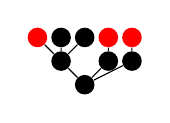
\begin{tikzpicture}[scale=.2]
\node[circle, scale=0.75, fill] (tid0) at (3.75,1.5){};
\node[circle, scale=0.75, fill] (tid1) at (2.25,3){};
\node[circle, scale=0.75, fill, red] (tid4) at (0.75,4.5){};
\node[circle, scale=0.75, fill] (tid5) at (2.25,4.5){};
\node[circle, scale=0.75, fill] (tid6) at (3.75,4.5){};
\draw[](tid1) -- (tid4);
\draw[](tid1) -- (tid5);
\draw[](tid1) -- (tid6);
\node[circle, scale=0.75, fill] (tid2) at (5.25,3){};
\node[circle, scale=0.75, fill, red] (tid7) at (5.25,4.5){};
\draw[](tid2) -- (tid7);
\node[circle, scale=0.75, fill] (tid3) at (6.75,3){};
\node[circle, scale=0.75, fill, red] (tid8) at (6.75,4.5){};
\draw[](tid3) -- (tid8);
\draw[](tid0) -- (tid1);
\draw[](tid0) -- (tid2);
\draw[](tid0) -- (tid3);
\end{tikzpicture}
\nodepart{two}
\footnotesize{4.92029}
\nodepart{three}
\footnotesize{$33\:22\:44$}
};
 & 
\node[draw=black, rectangle split,  rectangle split parts=3] (sn0x21cd300){
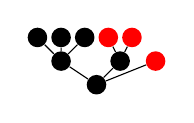
\begin{tikzpicture}[scale=.2]
\node[circle, scale=0.75, fill] (tid0) at (4.5,1.5){};
\node[circle, scale=0.75, fill] (tid1) at (2.25,3){};
\node[circle, scale=0.75, fill] (tid4) at (0.75,4.5){};
\node[circle, scale=0.75, fill] (tid5) at (2.25,4.5){};
\node[circle, scale=0.75, fill] (tid6) at (3.75,4.5){};
\draw[](tid1) -- (tid4);
\draw[](tid1) -- (tid5);
\draw[](tid1) -- (tid6);
\node[circle, scale=0.75, fill] (tid2) at (6,3){};
\node[circle, scale=0.75, fill, red] (tid7) at (5.25,4.5){};
\node[circle, scale=0.75, fill, red] (tid8) at (6.75,4.5){};
\draw[](tid2) -- (tid7);
\draw[](tid2) -- (tid8);
\node[circle, scale=0.75, fill, red] (tid3) at (8.25,3){};
\draw[](tid0) -- (tid1);
\draw[](tid0) -- (tid2);
\draw[](tid0) -- (tid3);
\end{tikzpicture}
\nodepart{two}
\footnotesize{5.00503}
\nodepart{three}
\footnotesize{$67\:33$}
};
 & 
\node[draw=black, rectangle split,  rectangle split parts=3] (sn0x21ce0b0){
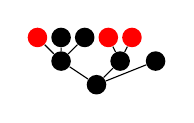
\begin{tikzpicture}[scale=.2]
\node[circle, scale=0.75, fill] (tid0) at (4.5,1.5){};
\node[circle, scale=0.75, fill] (tid1) at (2.25,3){};
\node[circle, scale=0.75, fill, red] (tid4) at (0.75,4.5){};
\node[circle, scale=0.75, fill] (tid5) at (2.25,4.5){};
\node[circle, scale=0.75, fill] (tid6) at (3.75,4.5){};
\draw[](tid1) -- (tid4);
\draw[](tid1) -- (tid5);
\draw[](tid1) -- (tid6);
\node[circle, scale=0.75, fill] (tid2) at (6,3){};
\node[circle, scale=0.75, fill, red] (tid7) at (5.25,4.5){};
\node[circle, scale=0.75, fill, red] (tid8) at (6.75,4.5){};
\draw[](tid2) -- (tid7);
\draw[](tid2) -- (tid8);
\node[circle, scale=0.75, fill] (tid3) at (8.25,3){};
\draw[](tid0) -- (tid1);
\draw[](tid0) -- (tid2);
\draw[](tid0) -- (tid3);
\end{tikzpicture}
\nodepart{two}
\footnotesize{4.93126}
\nodepart{three}
\footnotesize{$22\:44\:11\:22$}
};
 & 
\\
};
\end{scope}
\begin{scope}[yshift=\leveltopIII cm]
\matrix (line3) [column sep=1cm] {
\node[draw=black, rectangle split,  rectangle split parts=3] (sn0x21ce180){
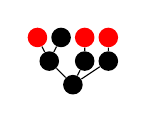
\begin{tikzpicture}[scale=.2]
\node[circle, scale=0.75, fill] (tid0) at (3,1.5){};
\node[circle, scale=0.75, fill] (tid1) at (1.5,3){};
\node[circle, scale=0.75, fill, red] (tid4) at (0.75,4.5){};
\node[circle, scale=0.75, fill] (tid5) at (2.25,4.5){};
\draw[](tid1) -- (tid4);
\draw[](tid1) -- (tid5);
\node[circle, scale=0.75, fill] (tid2) at (3.75,3){};
\node[circle, scale=0.75, fill, red] (tid6) at (3.75,4.5){};
\draw[](tid2) -- (tid6);
\node[circle, scale=0.75, fill] (tid3) at (5.25,3){};
\node[circle, scale=0.75, fill, red] (tid7) at (5.25,4.5){};
\draw[](tid3) -- (tid7);
\draw[](tid0) -- (tid1);
\draw[](tid0) -- (tid2);
\draw[](tid0) -- (tid3);
\end{tikzpicture}
\nodepart{two}
\footnotesize{4.56379}
\nodepart{three}
\footnotesize{$33\:33\:33$}
};
 & 
\node[draw=black, rectangle split,  rectangle split parts=3] (sn0x21ce430){
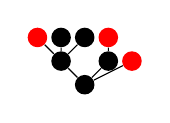
\begin{tikzpicture}[scale=.2]
\node[circle, scale=0.75, fill] (tid0) at (3.75,1.5){};
\node[circle, scale=0.75, fill] (tid1) at (2.25,3){};
\node[circle, scale=0.75, fill, red] (tid4) at (0.75,4.5){};
\node[circle, scale=0.75, fill] (tid5) at (2.25,4.5){};
\node[circle, scale=0.75, fill] (tid6) at (3.75,4.5){};
\draw[](tid1) -- (tid4);
\draw[](tid1) -- (tid5);
\draw[](tid1) -- (tid6);
\node[circle, scale=0.75, fill] (tid2) at (5.25,3){};
\node[circle, scale=0.75, fill, red] (tid7) at (5.25,4.5){};
\draw[](tid2) -- (tid7);
\node[circle, scale=0.75, fill, red] (tid3) at (6.75,3){};
\draw[](tid0) -- (tid1);
\draw[](tid0) -- (tid2);
\draw[](tid0) -- (tid3);
\end{tikzpicture}
\nodepart{two}
\footnotesize{4.64952}
\nodepart{three}
\footnotesize{$33\:33\:11\:22$}
};
 & 
\node[draw=black, rectangle split,  rectangle split parts=3] (sn0x21ce760){
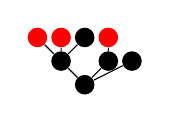
\begin{tikzpicture}[scale=.2]
\node[circle, scale=0.75, fill] (tid0) at (3.75,1.5){};
\node[circle, scale=0.75, fill] (tid1) at (2.25,3){};
\node[circle, scale=0.75, fill, red] (tid4) at (0.75,4.5){};
\node[circle, scale=0.75, fill, red] (tid5) at (2.25,4.5){};
\node[circle, scale=0.75, fill] (tid6) at (3.75,4.5){};
\draw[](tid1) -- (tid4);
\draw[](tid1) -- (tid5);
\draw[](tid1) -- (tid6);
\node[circle, scale=0.75, fill] (tid2) at (5.25,3){};
\node[circle, scale=0.75, fill, red] (tid7) at (5.25,4.5){};
\draw[](tid2) -- (tid7);
\node[circle, scale=0.75, fill] (tid3) at (6.75,3){};
\draw[](tid0) -- (tid1);
\draw[](tid0) -- (tid2);
\draw[](tid0) -- (tid3);
\end{tikzpicture}
\nodepart{two}
\footnotesize{4.57305}
\nodepart{three}
\footnotesize{$33\:33\:22\:11$}
};
 & 
\node[draw=black, rectangle split,  rectangle split parts=3] (sn0x21d4740){
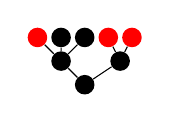
\begin{tikzpicture}[scale=.2]
\node[circle, scale=0.75, fill] (tid0) at (3.75,1.5){};
\node[circle, scale=0.75, fill] (tid1) at (2.25,3){};
\node[circle, scale=0.75, fill, red] (tid3) at (0.75,4.5){};
\node[circle, scale=0.75, fill] (tid4) at (2.25,4.5){};
\node[circle, scale=0.75, fill] (tid5) at (3.75,4.5){};
\draw[](tid1) -- (tid3);
\draw[](tid1) -- (tid4);
\draw[](tid1) -- (tid5);
\node[circle, scale=0.75, fill] (tid2) at (6,3){};
\node[circle, scale=0.75, fill, red] (tid6) at (5.25,4.5){};
\node[circle, scale=0.75, fill, red] (tid7) at (6.75,4.5){};
\draw[](tid2) -- (tid6);
\draw[](tid2) -- (tid7);
\draw[](tid0) -- (tid1);
\draw[](tid0) -- (tid2);
\end{tikzpicture}
\nodepart{two}
\footnotesize{4.71605}
\nodepart{three}
\footnotesize{$67\:33$}
};
 & 
\node[draw=black, rectangle split,  rectangle split parts=3] (sn0x21d53d0){
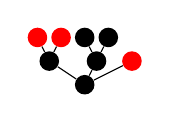
\begin{tikzpicture}[scale=.2]
\node[circle, scale=0.75, fill] (tid0) at (3.75,1.5){};
\node[circle, scale=0.75, fill] (tid1) at (1.5,3){};
\node[circle, scale=0.75, fill, red] (tid4) at (0.75,4.5){};
\node[circle, scale=0.75, fill, red] (tid5) at (2.25,4.5){};
\draw[](tid1) -- (tid4);
\draw[](tid1) -- (tid5);
\node[circle, scale=0.75, fill] (tid2) at (4.5,3){};
\node[circle, scale=0.75, fill] (tid6) at (3.75,4.5){};
\node[circle, scale=0.75, fill] (tid7) at (5.25,4.5){};
\draw[](tid2) -- (tid6);
\draw[](tid2) -- (tid7);
\node[circle, scale=0.75, fill, red] (tid3) at (6.75,3){};
\draw[](tid0) -- (tid1);
\draw[](tid0) -- (tid2);
\draw[](tid0) -- (tid3);
\end{tikzpicture}
\nodepart{two}
\footnotesize{4.64609}
\nodepart{three}
\footnotesize{$67\:33$}
};
 & 
\node[draw=black, rectangle split,  rectangle split parts=3] (sn0x21d54e0){
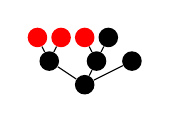
\begin{tikzpicture}[scale=.2]
\node[circle, scale=0.75, fill] (tid0) at (3.75,1.5){};
\node[circle, scale=0.75, fill] (tid1) at (1.5,3){};
\node[circle, scale=0.75, fill, red] (tid4) at (0.75,4.5){};
\node[circle, scale=0.75, fill, red] (tid5) at (2.25,4.5){};
\draw[](tid1) -- (tid4);
\draw[](tid1) -- (tid5);
\node[circle, scale=0.75, fill] (tid2) at (4.5,3){};
\node[circle, scale=0.75, fill, red] (tid6) at (3.75,4.5){};
\node[circle, scale=0.75, fill] (tid7) at (5.25,4.5){};
\draw[](tid2) -- (tid6);
\draw[](tid2) -- (tid7);
\node[circle, scale=0.75, fill] (tid3) at (6.75,3){};
\draw[](tid0) -- (tid1);
\draw[](tid0) -- (tid2);
\draw[](tid0) -- (tid3);
\end{tikzpicture}
\nodepart{two}
\footnotesize{4.57202}
\nodepart{three}
\footnotesize{$33\:50\:17$}
};
 & 
\\
};
\end{scope}
\begin{scope}[yshift=\leveltopIIII cm]
\matrix (line4) [column sep=1cm] {
\node[draw=black, rectangle split,  rectangle split parts=3] (sn0x21ce250){
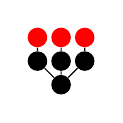
\begin{tikzpicture}[scale=.2]
\node[circle, scale=0.75, fill] (tid0) at (2.25,1.5){};
\node[circle, scale=0.75, fill] (tid1) at (0.75,3){};
\node[circle, scale=0.75, fill, red] (tid4) at (0.75,4.5){};
\draw[](tid1) -- (tid4);
\node[circle, scale=0.75, fill] (tid2) at (2.25,3){};
\node[circle, scale=0.75, fill, red] (tid5) at (2.25,4.5){};
\draw[](tid2) -- (tid5);
\node[circle, scale=0.75, fill] (tid3) at (3.75,3){};
\node[circle, scale=0.75, fill, red] (tid6) at (3.75,4.5){};
\draw[](tid3) -- (tid6);
\draw[](tid0) -- (tid1);
\draw[](tid0) -- (tid2);
\draw[](tid0) -- (tid3);
\end{tikzpicture}
\nodepart{two}
\footnotesize{4.21296}
\nodepart{three}
\footnotesize{$1$}
};
 & 
\node[draw=black, rectangle split,  rectangle split parts=3] (sn0x21ceae0){
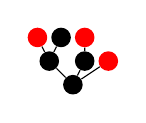
\begin{tikzpicture}[scale=.2]
\node[circle, scale=0.75, fill] (tid0) at (3,1.5){};
\node[circle, scale=0.75, fill] (tid1) at (1.5,3){};
\node[circle, scale=0.75, fill, red] (tid4) at (0.75,4.5){};
\node[circle, scale=0.75, fill] (tid5) at (2.25,4.5){};
\draw[](tid1) -- (tid4);
\draw[](tid1) -- (tid5);
\node[circle, scale=0.75, fill] (tid2) at (3.75,3){};
\node[circle, scale=0.75, fill, red] (tid6) at (3.75,4.5){};
\draw[](tid2) -- (tid6);
\node[circle, scale=0.75, fill, red] (tid3) at (5.25,3){};
\draw[](tid0) -- (tid1);
\draw[](tid0) -- (tid2);
\draw[](tid0) -- (tid3);
\end{tikzpicture}
\nodepart{two}
\footnotesize{4.27469}
\nodepart{three}
\footnotesize{$33\:33\:17\:17$}
};
 & 
\node[draw=black, rectangle split,  rectangle split parts=3] (sn0x21cf5a0){
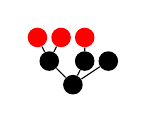
\begin{tikzpicture}[scale=.2]
\node[circle, scale=0.75, fill] (tid0) at (3,1.5){};
\node[circle, scale=0.75, fill] (tid1) at (1.5,3){};
\node[circle, scale=0.75, fill, red] (tid4) at (0.75,4.5){};
\node[circle, scale=0.75, fill, red] (tid5) at (2.25,4.5){};
\draw[](tid1) -- (tid4);
\draw[](tid1) -- (tid5);
\node[circle, scale=0.75, fill] (tid2) at (3.75,3){};
\node[circle, scale=0.75, fill, red] (tid6) at (3.75,4.5){};
\draw[](tid2) -- (tid6);
\node[circle, scale=0.75, fill] (tid3) at (5.25,3){};
\draw[](tid0) -- (tid1);
\draw[](tid0) -- (tid2);
\draw[](tid0) -- (tid3);
\end{tikzpicture}
\nodepart{two}
\footnotesize{4.2037}
\nodepart{three}
\footnotesize{$67\:33$}
};
 & 
\node[draw=black, rectangle split,  rectangle split parts=3] (sn0x21d22d0){
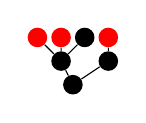
\begin{tikzpicture}[scale=.2]
\node[circle, scale=0.75, fill] (tid0) at (3,1.5){};
\node[circle, scale=0.75, fill] (tid1) at (2.25,3){};
\node[circle, scale=0.75, fill, red] (tid3) at (0.75,4.5){};
\node[circle, scale=0.75, fill, red] (tid4) at (2.25,4.5){};
\node[circle, scale=0.75, fill] (tid5) at (3.75,4.5){};
\draw[](tid1) -- (tid3);
\draw[](tid1) -- (tid4);
\draw[](tid1) -- (tid5);
\node[circle, scale=0.75, fill] (tid2) at (5.25,3){};
\node[circle, scale=0.75, fill, red] (tid6) at (5.25,4.5){};
\draw[](tid2) -- (tid6);
\draw[](tid0) -- (tid1);
\draw[](tid0) -- (tid2);
\end{tikzpicture}
\nodepart{two}
\footnotesize{4.37963}
\nodepart{three}
\footnotesize{$67\:17\:17$}
};
 & 
\node[draw=black, rectangle split,  rectangle split parts=3] (sn0x21d2ce0){
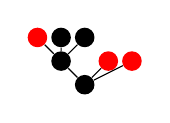
\begin{tikzpicture}[scale=.2]
\node[circle, scale=0.75, fill] (tid0) at (3.75,1.5){};
\node[circle, scale=0.75, fill] (tid1) at (2.25,3){};
\node[circle, scale=0.75, fill, red] (tid4) at (0.75,4.5){};
\node[circle, scale=0.75, fill] (tid5) at (2.25,4.5){};
\node[circle, scale=0.75, fill] (tid6) at (3.75,4.5){};
\draw[](tid1) -- (tid4);
\draw[](tid1) -- (tid5);
\draw[](tid1) -- (tid6);
\node[circle, scale=0.75, fill, red] (tid2) at (5.25,3){};
\node[circle, scale=0.75, fill, red] (tid3) at (6.75,3){};
\draw[](tid0) -- (tid1);
\draw[](tid0) -- (tid2);
\draw[](tid0) -- (tid3);
\end{tikzpicture}
\nodepart{two}
\footnotesize{4.34568}
\nodepart{three}
\footnotesize{$33\:67$}
};
 & 
\node[draw=black, rectangle split,  rectangle split parts=3] (sn0x21d3130){
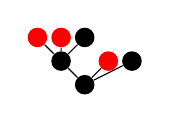
\begin{tikzpicture}[scale=.2]
\node[circle, scale=0.75, fill] (tid0) at (3.75,1.5){};
\node[circle, scale=0.75, fill] (tid1) at (2.25,3){};
\node[circle, scale=0.75, fill, red] (tid4) at (0.75,4.5){};
\node[circle, scale=0.75, fill, red] (tid5) at (2.25,4.5){};
\node[circle, scale=0.75, fill] (tid6) at (3.75,4.5){};
\draw[](tid1) -- (tid4);
\draw[](tid1) -- (tid5);
\draw[](tid1) -- (tid6);
\node[circle, scale=0.75, fill, red] (tid2) at (5.25,3){};
\node[circle, scale=0.75, fill] (tid3) at (6.75,3){};
\draw[](tid0) -- (tid1);
\draw[](tid0) -- (tid2);
\draw[](tid0) -- (tid3);
\end{tikzpicture}
\nodepart{two}
\footnotesize{4.26852}
\nodepart{three}
\footnotesize{$33\:33\:17\:17$}
};
 & 
\node[draw=black, rectangle split,  rectangle split parts=3] (sn0x21d4280){
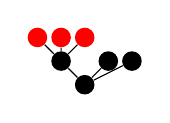
\begin{tikzpicture}[scale=.2]
\node[circle, scale=0.75, fill] (tid0) at (3.75,1.5){};
\node[circle, scale=0.75, fill] (tid1) at (2.25,3){};
\node[circle, scale=0.75, fill, red] (tid4) at (0.75,4.5){};
\node[circle, scale=0.75, fill, red] (tid5) at (2.25,4.5){};
\node[circle, scale=0.75, fill, red] (tid6) at (3.75,4.5){};
\draw[](tid1) -- (tid4);
\draw[](tid1) -- (tid5);
\draw[](tid1) -- (tid6);
\node[circle, scale=0.75, fill] (tid2) at (5.25,3){};
\node[circle, scale=0.75, fill] (tid3) at (6.75,3){};
\draw[](tid0) -- (tid1);
\draw[](tid0) -- (tid2);
\draw[](tid0) -- (tid3);
\end{tikzpicture}
\nodepart{two}
\footnotesize{4.18519}
\nodepart{three}
\footnotesize{$1$}
};
 & 
\node[draw=black, rectangle split,  rectangle split parts=3] (sn0x21d48e0){
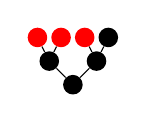
\begin{tikzpicture}[scale=.2]
\node[circle, scale=0.75, fill] (tid0) at (3,1.5){};
\node[circle, scale=0.75, fill] (tid1) at (1.5,3){};
\node[circle, scale=0.75, fill, red] (tid3) at (0.75,4.5){};
\node[circle, scale=0.75, fill, red] (tid4) at (2.25,4.5){};
\draw[](tid1) -- (tid3);
\draw[](tid1) -- (tid4);
\node[circle, scale=0.75, fill] (tid2) at (4.5,3){};
\node[circle, scale=0.75, fill, red] (tid5) at (3.75,4.5){};
\node[circle, scale=0.75, fill] (tid6) at (5.25,4.5){};
\draw[](tid2) -- (tid5);
\draw[](tid2) -- (tid6);
\draw[](tid0) -- (tid1);
\draw[](tid0) -- (tid2);
\end{tikzpicture}
\nodepart{two}
\footnotesize{4.38889}
\nodepart{three}
\footnotesize{$1$}
};
 & 
\node[draw=black, rectangle split,  rectangle split parts=3] (sn0x21d5e10){
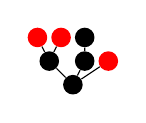
\begin{tikzpicture}[scale=.2]
\node[circle, scale=0.75, fill] (tid0) at (3,1.5){};
\node[circle, scale=0.75, fill] (tid1) at (1.5,3){};
\node[circle, scale=0.75, fill, red] (tid4) at (0.75,4.5){};
\node[circle, scale=0.75, fill, red] (tid5) at (2.25,4.5){};
\draw[](tid1) -- (tid4);
\draw[](tid1) -- (tid5);
\node[circle, scale=0.75, fill] (tid2) at (3.75,3){};
\node[circle, scale=0.75, fill] (tid6) at (3.75,4.5){};
\draw[](tid2) -- (tid6);
\node[circle, scale=0.75, fill, red] (tid3) at (5.25,3){};
\draw[](tid0) -- (tid1);
\draw[](tid0) -- (tid2);
\draw[](tid0) -- (tid3);
\end{tikzpicture}
\nodepart{two}
\footnotesize{4.27161}
\nodepart{three}
\footnotesize{$67\:33$}
};
 & 
\\
};
\end{scope}
\begin{scope}[yshift=\leveltopIIIII cm]
\matrix (line5) [column sep=1cm] {
\node[draw=black, rectangle split,  rectangle split parts=3] (sn0x21ced80){
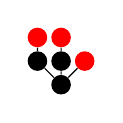
\begin{tikzpicture}[scale=.2]
\node[circle, scale=0.75, fill] (tid0) at (2.25,1.5){};
\node[circle, scale=0.75, fill] (tid1) at (0.75,3){};
\node[circle, scale=0.75, fill, red] (tid4) at (0.75,4.5){};
\draw[](tid1) -- (tid4);
\node[circle, scale=0.75, fill] (tid2) at (2.25,3){};
\node[circle, scale=0.75, fill, red] (tid5) at (2.25,4.5){};
\draw[](tid2) -- (tid5);
\node[circle, scale=0.75, fill, red] (tid3) at (3.75,3){};
\draw[](tid0) -- (tid1);
\draw[](tid0) -- (tid2);
\draw[](tid0) -- (tid3);
\end{tikzpicture}
\nodepart{two}
\footnotesize{3.87963}
\nodepart{three}
\footnotesize{$33\:67$}
};
 & 
\node[draw=black, rectangle split,  rectangle split parts=3] (sn0x21d0e50){
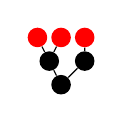
\begin{tikzpicture}[scale=.2]
\node[circle, scale=0.75, fill] (tid0) at (2.25,1.5){};
\node[circle, scale=0.75, fill] (tid1) at (1.5,3){};
\node[circle, scale=0.75, fill, red] (tid3) at (0.75,4.5){};
\node[circle, scale=0.75, fill, red] (tid4) at (2.25,4.5){};
\draw[](tid1) -- (tid3);
\draw[](tid1) -- (tid4);
\node[circle, scale=0.75, fill] (tid2) at (3.75,3){};
\node[circle, scale=0.75, fill, red] (tid5) at (3.75,4.5){};
\draw[](tid2) -- (tid5);
\draw[](tid0) -- (tid1);
\draw[](tid0) -- (tid2);
\end{tikzpicture}
\nodepart{two}
\footnotesize{4.05556}
\nodepart{three}
\footnotesize{$67\:33$}
};
 & 
\node[draw=black, rectangle split,  rectangle split parts=3] (sn0x21d0fa0){
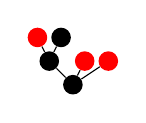
\begin{tikzpicture}[scale=.2]
\node[circle, scale=0.75, fill] (tid0) at (3,1.5){};
\node[circle, scale=0.75, fill] (tid1) at (1.5,3){};
\node[circle, scale=0.75, fill, red] (tid4) at (0.75,4.5){};
\node[circle, scale=0.75, fill] (tid5) at (2.25,4.5){};
\draw[](tid1) -- (tid4);
\draw[](tid1) -- (tid5);
\node[circle, scale=0.75, fill, red] (tid2) at (3.75,3){};
\node[circle, scale=0.75, fill, red] (tid3) at (5.25,3){};
\draw[](tid0) -- (tid1);
\draw[](tid0) -- (tid2);
\draw[](tid0) -- (tid3);
\end{tikzpicture}
\nodepart{two}
\footnotesize{3.92593}
\nodepart{three}
\footnotesize{$33\:67$}
};
 & 
\node[draw=black, rectangle split,  rectangle split parts=3] (sn0x21d19a0){
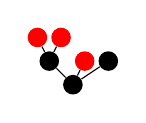
\begin{tikzpicture}[scale=.2]
\node[circle, scale=0.75, fill] (tid0) at (3,1.5){};
\node[circle, scale=0.75, fill] (tid1) at (1.5,3){};
\node[circle, scale=0.75, fill, red] (tid4) at (0.75,4.5){};
\node[circle, scale=0.75, fill, red] (tid5) at (2.25,4.5){};
\draw[](tid1) -- (tid4);
\draw[](tid1) -- (tid5);
\node[circle, scale=0.75, fill, red] (tid2) at (3.75,3){};
\node[circle, scale=0.75, fill] (tid3) at (5.25,3){};
\draw[](tid0) -- (tid1);
\draw[](tid0) -- (tid2);
\draw[](tid0) -- (tid3);
\end{tikzpicture}
\nodepart{two}
\footnotesize{3.85185}
\nodepart{three}
\footnotesize{$67\:33$}
};
 & 
\node[draw=black, rectangle split,  rectangle split parts=3] (sn0x21d36b0){
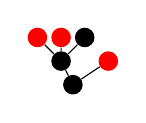
\begin{tikzpicture}[scale=.2]
\node[circle, scale=0.75, fill] (tid0) at (3,1.5){};
\node[circle, scale=0.75, fill] (tid1) at (2.25,3){};
\node[circle, scale=0.75, fill, red] (tid3) at (0.75,4.5){};
\node[circle, scale=0.75, fill, red] (tid4) at (2.25,4.5){};
\node[circle, scale=0.75, fill] (tid5) at (3.75,4.5){};
\draw[](tid1) -- (tid3);
\draw[](tid1) -- (tid4);
\draw[](tid1) -- (tid5);
\node[circle, scale=0.75, fill, red] (tid2) at (5.25,3){};
\draw[](tid0) -- (tid1);
\draw[](tid0) -- (tid2);
\end{tikzpicture}
\nodepart{two}
\footnotesize{4.05556}
\nodepart{three}
\footnotesize{$67\:33$}
};
 & 
\node[draw=black, rectangle split,  rectangle split parts=3] (sn0x21d34d0){
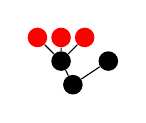
\begin{tikzpicture}[scale=.2]
\node[circle, scale=0.75, fill] (tid0) at (3,1.5){};
\node[circle, scale=0.75, fill] (tid1) at (2.25,3){};
\node[circle, scale=0.75, fill, red] (tid3) at (0.75,4.5){};
\node[circle, scale=0.75, fill, red] (tid4) at (2.25,4.5){};
\node[circle, scale=0.75, fill, red] (tid5) at (3.75,4.5){};
\draw[](tid1) -- (tid3);
\draw[](tid1) -- (tid4);
\draw[](tid1) -- (tid5);
\node[circle, scale=0.75, fill] (tid2) at (5.25,3){};
\draw[](tid0) -- (tid1);
\draw[](tid0) -- (tid2);
\end{tikzpicture}
\nodepart{two}
\footnotesize{4}
\nodepart{three}
\footnotesize{$1$}
};
 & 
\\
};
\end{scope}
\begin{scope}[yshift=\leveltopIIIIII cm]
\matrix (line6) [column sep=1cm] {
\node[draw=black, rectangle split,  rectangle split parts=3] (sn0x21cfc10){
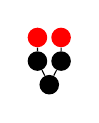
\begin{tikzpicture}[scale=.2]
\node[circle, scale=0.75, fill] (tid0) at (1.5,1.5){};
\node[circle, scale=0.75, fill] (tid1) at (0.75,3){};
\node[circle, scale=0.75, fill, red] (tid3) at (0.75,4.5){};
\draw[](tid1) -- (tid3);
\node[circle, scale=0.75, fill] (tid2) at (2.25,3){};
\node[circle, scale=0.75, fill, red] (tid4) at (2.25,4.5){};
\draw[](tid2) -- (tid4);
\draw[](tid0) -- (tid1);
\draw[](tid0) -- (tid2);
\end{tikzpicture}
\nodepart{two}
\footnotesize{3.75}
\nodepart{three}
\footnotesize{$1$}
};
 & 
\node[draw=black, rectangle split,  rectangle split parts=3] (sn0x21cdc20){
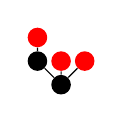
\begin{tikzpicture}[scale=.2]
\node[circle, scale=0.75, fill] (tid0) at (2.25,1.5){};
\node[circle, scale=0.75, fill] (tid1) at (0.75,3){};
\node[circle, scale=0.75, fill, red] (tid4) at (0.75,4.5){};
\draw[](tid1) -- (tid4);
\node[circle, scale=0.75, fill, red] (tid2) at (2.25,3){};
\node[circle, scale=0.75, fill, red] (tid3) at (3.75,3){};
\draw[](tid0) -- (tid1);
\draw[](tid0) -- (tid2);
\draw[](tid0) -- (tid3);
\end{tikzpicture}
\nodepart{two}
\footnotesize{3.44444}
\nodepart{three}
\footnotesize{$67\:33$}
};
 & 
\node[draw=black, rectangle split,  rectangle split parts=3] (sn0x21d1cc0){
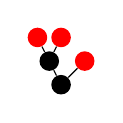
\begin{tikzpicture}[scale=.2]
\node[circle, scale=0.75, fill] (tid0) at (2.25,1.5){};
\node[circle, scale=0.75, fill] (tid1) at (1.5,3){};
\node[circle, scale=0.75, fill, red] (tid3) at (0.75,4.5){};
\node[circle, scale=0.75, fill, red] (tid4) at (2.25,4.5){};
\draw[](tid1) -- (tid3);
\draw[](tid1) -- (tid4);
\node[circle, scale=0.75, fill, red] (tid2) at (3.75,3){};
\draw[](tid0) -- (tid1);
\draw[](tid0) -- (tid2);
\end{tikzpicture}
\nodepart{two}
\footnotesize{3.66667}
\nodepart{three}
\footnotesize{$67\:33$}
};
 & 
\node[draw=black, rectangle split,  rectangle split parts=3] (sn0x21d3bb0){
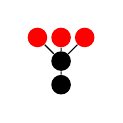
\begin{tikzpicture}[scale=.2]
\node[circle, scale=0.75, fill] (tid0) at (2.25,1.5){};
\node[circle, scale=0.75, fill] (tid1) at (2.25,3){};
\node[circle, scale=0.75, fill, red] (tid2) at (0.75,4.5){};
\node[circle, scale=0.75, fill, red] (tid3) at (2.25,4.5){};
\node[circle, scale=0.75, fill, red] (tid4) at (3.75,4.5){};
\draw[](tid1) -- (tid2);
\draw[](tid1) -- (tid3);
\draw[](tid1) -- (tid4);
\draw[](tid0) -- (tid1);
\end{tikzpicture}
\nodepart{two}
\footnotesize{3.83333}
\nodepart{three}
\footnotesize{$1$}
};
 & 
\\
};
\end{scope}
\begin{scope}[yshift=\leveltopIIIIIII cm]
\matrix (line7) [column sep=1cm] {
\node[draw=black, rectangle split,  rectangle split parts=3] (sn0x21cfd50){
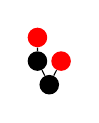
\begin{tikzpicture}[scale=.2]
\node[circle, scale=0.75, fill] (tid0) at (1.5,1.5){};
\node[circle, scale=0.75, fill] (tid1) at (0.75,3){};
\node[circle, scale=0.75, fill, red] (tid3) at (0.75,4.5){};
\draw[](tid1) -- (tid3);
\node[circle, scale=0.75, fill, red] (tid2) at (2.25,3){};
\draw[](tid0) -- (tid1);
\draw[](tid0) -- (tid2);
\end{tikzpicture}
\nodepart{two}
\footnotesize{3.25}
\nodepart{three}
\footnotesize{$50\:50$}
};
 & 
\node[draw=black, rectangle split,  rectangle split parts=3] (sn0x21d06a0){
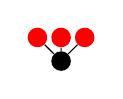
\begin{tikzpicture}[scale=.2]
\node[circle, scale=0.75, fill] (tid0) at (2.25,1.5){};
\node[circle, scale=0.75, fill, red] (tid1) at (0.75,3){};
\node[circle, scale=0.75, fill, red] (tid2) at (2.25,3){};
\node[circle, scale=0.75, fill, red] (tid3) at (3.75,3){};
\draw[](tid0) -- (tid1);
\draw[](tid0) -- (tid2);
\draw[](tid0) -- (tid3);
\end{tikzpicture}
\nodepart{two}
\footnotesize{2.83333}
\nodepart{three}
\footnotesize{$1$}
};
 & 
\node[draw=black, rectangle split,  rectangle split parts=3] (sn0x21d1160){
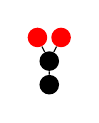
\begin{tikzpicture}[scale=.2]
\node[circle, scale=0.75, fill] (tid0) at (1.5,1.5){};
\node[circle, scale=0.75, fill] (tid1) at (1.5,3){};
\node[circle, scale=0.75, fill, red] (tid2) at (0.75,4.5){};
\node[circle, scale=0.75, fill, red] (tid3) at (2.25,4.5){};
\draw[](tid1) -- (tid2);
\draw[](tid1) -- (tid3);
\draw[](tid0) -- (tid1);
\end{tikzpicture}
\nodepart{two}
\footnotesize{3.5}
\nodepart{three}
\footnotesize{$1$}
};
 & 
\\
};
\end{scope}
\begin{scope}[yshift=\leveltopIIIIIIII cm]
\matrix (line8) [column sep=1cm] {
\node[draw=black, rectangle split,  rectangle split parts=3] (sn0x21cfe20){
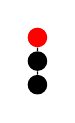
\begin{tikzpicture}[scale=.2]
\node[circle, scale=0.75, fill] (tid0) at (0.75,1.5){};
\node[circle, scale=0.75, fill] (tid1) at (0.75,3){};
\node[circle, scale=0.75, fill, red] (tid2) at (0.75,4.5){};
\draw[](tid1) -- (tid2);
\draw[](tid0) -- (tid1);
\end{tikzpicture}
\nodepart{two}
\footnotesize{3}
\nodepart{three}
\footnotesize{$1$}
};
 & 
\node[draw=black, rectangle split,  rectangle split parts=3] (sn0x21cfef0){

\begin{tikzpicture}[scale=.2]
\node[circle, scale=0.75, fill] (tid0) at (1.5,1.5){};
\node[circle, scale=0.75, fill, red] (tid1) at (0.75,3){};
\node[circle, scale=0.75, fill, red] (tid2) at (2.25,3){};
\draw[](tid0) -- (tid1);
\draw[](tid0) -- (tid2);
\end{tikzpicture}
\nodepart{two}
\footnotesize{2.5}
\nodepart{three}
\footnotesize{$1$}
};
 & 
\\
};
\end{scope}
\begin{scope}[yshift=\leveltopIIIIIIIII cm]
\matrix (line9) [column sep=1cm] {
\node[draw=black, rectangle split,  rectangle split parts=3] (sn0x21cffc0){

\begin{tikzpicture}[scale=.2]
\node[circle, scale=0.75, fill] (tid0) at (0.75,1.5){};
\node[circle, scale=0.75, fill, red] (tid1) at (0.75,3){};
\draw[](tid0) -- (tid1);
\end{tikzpicture}
\nodepart{two}
\footnotesize{2}
\nodepart{three}
\footnotesize{$1$}
};
 & 
\\
};
\end{scope}
\begin{scope}[yshift=\leveltopIIIIIIIIII cm]
\matrix (line10) [column sep=1cm] {
\node[draw=black, rectangle split,  rectangle split parts=3] (sn0x21d0090){

\begin{tikzpicture}[scale=.2]
\node[circle, scale=0.75, fill, red] (tid0) at (0.75,1.5){};
\end{tikzpicture}
\nodepart{two}
\footnotesize{1}
\nodepart{three}
\footnotesize{$$}
};
 & 
\\
};
\end{scope}
\begin{scope}[yshift=\leveltopIIIIIIIIIII cm]
\matrix (line11) [column sep=1cm] {
\\
};
\end{scope}
\draw (sn0x21a5ae0.south) -- (sn0x21ccf90.north);
\draw (sn0x21a5ae0.south) -- (sn0x21cd300.north);
\draw (sn0x21a5ae0.south) -- (sn0x21ce0b0.north);
\draw (sn0x21ccf90.south) -- (sn0x21ce180.north);
\draw (sn0x21ccf90.south) -- (sn0x21ce430.north);
\draw (sn0x21ccf90.south) -- (sn0x21ce760.north);
\draw (sn0x21cd300.south) -- (sn0x21d4740.north);
\draw (sn0x21cd300.south) -- (sn0x21ce430.north);
\draw (sn0x21ce0b0.south) -- (sn0x21d53d0.north);
\draw (sn0x21ce0b0.south) -- (sn0x21d54e0.north);
\draw (sn0x21ce0b0.south) -- (sn0x21ce430.north);
\draw (sn0x21ce0b0.south) -- (sn0x21ce760.north);
\draw (sn0x21ce180.south) -- (sn0x21ce250.north);
\draw (sn0x21ce180.south) -- (sn0x21ceae0.north);
\draw (sn0x21ce180.south) -- (sn0x21cf5a0.north);
\draw (sn0x21ce430.south) -- (sn0x21d22d0.north);
\draw (sn0x21ce430.south) -- (sn0x21ceae0.north);
\draw (sn0x21ce430.south) -- (sn0x21d2ce0.north);
\draw (sn0x21ce430.south) -- (sn0x21d3130.north);
\draw (sn0x21ce760.south) -- (sn0x21ceae0.north);
\draw (sn0x21ce760.south) -- (sn0x21cf5a0.north);
\draw (sn0x21ce760.south) -- (sn0x21d3130.north);
\draw (sn0x21ce760.south) -- (sn0x21d4280.north);
\draw (sn0x21d4740.south) -- (sn0x21d48e0.north);
\draw (sn0x21d4740.south) -- (sn0x21d22d0.north);
\draw (sn0x21d53d0.south) -- (sn0x21d48e0.north);
\draw (sn0x21d53d0.south) -- (sn0x21ceae0.north);
\draw (sn0x21d54e0.south) -- (sn0x21ceae0.north);
\draw (sn0x21d54e0.south) -- (sn0x21cf5a0.north);
\draw (sn0x21d54e0.south) -- (sn0x21d5e10.north);
\draw (sn0x21ce250.south) -- (sn0x21ced80.north);
\draw (sn0x21ceae0.south) -- (sn0x21d0e50.north);
\draw (sn0x21ceae0.south) -- (sn0x21ced80.north);
\draw (sn0x21ceae0.south) -- (sn0x21d0fa0.north);
\draw (sn0x21ceae0.south) -- (sn0x21d19a0.north);
\draw (sn0x21cf5a0.south) -- (sn0x21ced80.north);
\draw (sn0x21cf5a0.south) -- (sn0x21d19a0.north);
\draw (sn0x21d22d0.south) -- (sn0x21d0e50.north);
\draw (sn0x21d22d0.south) -- (sn0x21d36b0.north);
\draw (sn0x21d22d0.south) -- (sn0x21d34d0.north);
\draw (sn0x21d2ce0.south) -- (sn0x21d36b0.north);
\draw (sn0x21d2ce0.south) -- (sn0x21d0fa0.north);
\draw (sn0x21d3130.south) -- (sn0x21d36b0.north);
\draw (sn0x21d3130.south) -- (sn0x21d34d0.north);
\draw (sn0x21d3130.south) -- (sn0x21d0fa0.north);
\draw (sn0x21d3130.south) -- (sn0x21d19a0.north);
\draw (sn0x21d4280.south) -- (sn0x21d19a0.north);
\draw (sn0x21d48e0.south) -- (sn0x21d0e50.north);
\draw (sn0x21d5e10.south) -- (sn0x21d0e50.north);
\draw (sn0x21d5e10.south) -- (sn0x21ced80.north);
\draw (sn0x21ced80.south) -- (sn0x21cfc10.north);
\draw (sn0x21ced80.south) -- (sn0x21cdc20.north);
\draw (sn0x21d0e50.south) -- (sn0x21cfc10.north);
\draw (sn0x21d0e50.south) -- (sn0x21d1cc0.north);
\draw (sn0x21d0fa0.south) -- (sn0x21d1cc0.north);
\draw (sn0x21d0fa0.south) -- (sn0x21cdc20.north);
\draw (sn0x21d19a0.south) -- (sn0x21d1cc0.north);
\draw (sn0x21d19a0.south) -- (sn0x21cdc20.north);
\draw (sn0x21d36b0.south) -- (sn0x21d3bb0.north);
\draw (sn0x21d36b0.south) -- (sn0x21d1cc0.north);
\draw (sn0x21d34d0.south) -- (sn0x21d1cc0.north);
\draw (sn0x21cfc10.south) -- (sn0x21cfd50.north);
\draw (sn0x21cdc20.south) -- (sn0x21cfd50.north);
\draw (sn0x21cdc20.south) -- (sn0x21d06a0.north);
\draw (sn0x21d1cc0.south) -- (sn0x21d1160.north);
\draw (sn0x21d1cc0.south) -- (sn0x21cfd50.north);
\draw (sn0x21d3bb0.south) -- (sn0x21d1160.north);
\draw (sn0x21cfd50.south) -- (sn0x21cfe20.north);
\draw (sn0x21cfd50.south) -- (sn0x21cfef0.north);
\draw (sn0x21d06a0.south) -- (sn0x21cfef0.north);
\draw (sn0x21d1160.south) -- (sn0x21cfe20.north);
\draw (sn0x21cfe20.south) -- (sn0x21cffc0.north);
\draw (sn0x21cfef0.south) -- (sn0x21cffc0.north);
\draw (sn0x21cffc0.south) -- (sn0x21d0090.north);
\end{tikzpicture}

%%% Local Variables:
%%% TeX-master: "thesis/thesis.tex"
%%% End: 
\renewcommand{\leveltopI}{-15cm + \leveltop}
\renewcommand{\leveltopII}{-15cm + \leveltopI}
\renewcommand{\leveltopIII}{-15cm + \leveltopII}
\renewcommand{\leveltopIIII}{-15cm + \leveltopIII}
\renewcommand{\leveltopIIIII}{-15cm + \leveltopIIII}
\renewcommand{\leveltopIIIIII}{-15cm + \leveltopIIIII}
\renewcommand{\leveltopIIIIIII}{-15cm + \leveltopIIIIII}
\renewcommand{\leveltopIIIIIIII}{-15cm + \leveltopIIIIIII}
\renewcommand{\leveltopIIIIIIIII}{-15cm + \leveltopIIIIIIII}
\renewcommand{\leveltopIIIIIIIIII}{-15cm + \leveltopIIIIIIIII}
\begin{tikzpicture}[scale=.2, anchor=south]
\begin{scope}[yshift=\leveltopI cm]
\matrix (line1) [column sep=1cm] {
\node[draw=black, rectangle split,  rectangle split parts=3] (sn0x21cb130){
\begin{tikzpicture}[scale=.2]
\node[circle, scale=0.75, fill] (tid0) at (4.5,1.5){};
\node[circle, scale=0.75, fill] (tid1) at (2.25,3){};
\node[circle, scale=0.75, fill, red] (tid4) at (0.75,4.5){};
\node[circle, scale=0.75, fill, red] (tid5) at (2.25,4.5){};
\node[circle, scale=0.75, fill, red] (tid6) at (3.75,4.5){};
\draw[](tid1) -- (tid4);
\draw[](tid1) -- (tid5);
\draw[](tid1) -- (tid6);
\node[circle, scale=0.75, fill] (tid2) at (6,3){};
\node[circle, scale=0.75, fill] (tid7) at (5.25,4.5){};
\node[circle, scale=0.75, fill] (tid8) at (6.75,4.5){};
\draw[](tid2) -- (tid7);
\draw[](tid2) -- (tid8);
\node[circle, scale=0.75, fill] (tid3) at (8.25,3){};
\node[circle, scale=0.75, fill] (tid9) at (8.25,4.5){};
\draw[](tid3) -- (tid9);
\draw[](tid0) -- (tid1);
\draw[](tid0) -- (tid2);
\draw[](tid0) -- (tid3);
\end{tikzpicture}
\nodepart{two}
\footnotesize{5.23}
\nodepart{three}
\footnotesize{$67\:33$}
};
 & 
\\
};
\end{scope}
\begin{scope}[yshift=\leveltopII cm]
\matrix (line2) [column sep=1cm] {
\node[draw=black, rectangle split,  rectangle split parts=3] (sn0x21d62b0){
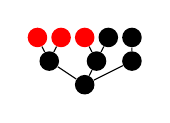
\begin{tikzpicture}[scale=.2]
\node[circle, scale=0.75, fill] (tid0) at (3.75,1.5){};
\node[circle, scale=0.75, fill] (tid1) at (1.5,3){};
\node[circle, scale=0.75, fill, red] (tid4) at (0.75,4.5){};
\node[circle, scale=0.75, fill, red] (tid5) at (2.25,4.5){};
\draw[](tid1) -- (tid4);
\draw[](tid1) -- (tid5);
\node[circle, scale=0.75, fill] (tid2) at (4.5,3){};
\node[circle, scale=0.75, fill, red] (tid6) at (3.75,4.5){};
\node[circle, scale=0.75, fill] (tid7) at (5.25,4.5){};
\draw[](tid2) -- (tid6);
\draw[](tid2) -- (tid7);
\node[circle, scale=0.75, fill] (tid3) at (6.75,3){};
\node[circle, scale=0.75, fill] (tid8) at (6.75,4.5){};
\draw[](tid3) -- (tid8);
\draw[](tid0) -- (tid1);
\draw[](tid0) -- (tid2);
\draw[](tid0) -- (tid3);
\end{tikzpicture}
\nodepart{two}
\footnotesize{4.89095}
\nodepart{three}
\footnotesize{$67\:33$}
};
 & 
\node[draw=black, rectangle split,  rectangle split parts=3] (sn0x21d6580){
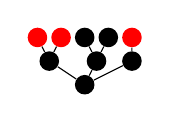
\begin{tikzpicture}[scale=.2]
\node[circle, scale=0.75, fill] (tid0) at (3.75,1.5){};
\node[circle, scale=0.75, fill] (tid1) at (1.5,3){};
\node[circle, scale=0.75, fill, red] (tid4) at (0.75,4.5){};
\node[circle, scale=0.75, fill, red] (tid5) at (2.25,4.5){};
\draw[](tid1) -- (tid4);
\draw[](tid1) -- (tid5);
\node[circle, scale=0.75, fill] (tid2) at (4.5,3){};
\node[circle, scale=0.75, fill] (tid6) at (3.75,4.5){};
\node[circle, scale=0.75, fill] (tid7) at (5.25,4.5){};
\draw[](tid2) -- (tid6);
\draw[](tid2) -- (tid7);
\node[circle, scale=0.75, fill] (tid3) at (6.75,3){};
\node[circle, scale=0.75, fill, red] (tid8) at (6.75,4.5){};
\draw[](tid3) -- (tid8);
\draw[](tid0) -- (tid1);
\draw[](tid0) -- (tid2);
\draw[](tid0) -- (tid3);
\end{tikzpicture}
\nodepart{two}
\footnotesize{4.90809}
\nodepart{three}
\footnotesize{$67\:11\:22$}
};
 & 
\\
};
\end{scope}
\begin{scope}[yshift=\leveltopIII cm]
\matrix (line3) [column sep=1cm] {
\node[draw=black, rectangle split,  rectangle split parts=3] (sn0x21d6cd0){
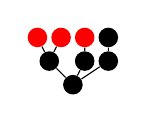
\begin{tikzpicture}[scale=.2]
\node[circle, scale=0.75, fill] (tid0) at (3,1.5){};
\node[circle, scale=0.75, fill] (tid1) at (1.5,3){};
\node[circle, scale=0.75, fill, red] (tid4) at (0.75,4.5){};
\node[circle, scale=0.75, fill, red] (tid5) at (2.25,4.5){};
\draw[](tid1) -- (tid4);
\draw[](tid1) -- (tid5);
\node[circle, scale=0.75, fill] (tid2) at (3.75,3){};
\node[circle, scale=0.75, fill, red] (tid6) at (3.75,4.5){};
\draw[](tid2) -- (tid6);
\node[circle, scale=0.75, fill] (tid3) at (5.25,3){};
\node[circle, scale=0.75, fill] (tid7) at (5.25,4.5){};
\draw[](tid3) -- (tid7);
\draw[](tid0) -- (tid1);
\draw[](tid0) -- (tid2);
\draw[](tid0) -- (tid3);
\end{tikzpicture}
\nodepart{two}
\footnotesize{4.55453}
\nodepart{three}
\footnotesize{$67\:17\:17$}
};
 & 
\node[draw=black, rectangle split,  rectangle split parts=3] (sn0x21ce180){
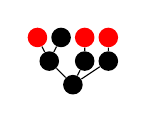
\begin{tikzpicture}[scale=.2]
\node[circle, scale=0.75, fill] (tid0) at (3,1.5){};
\node[circle, scale=0.75, fill] (tid1) at (1.5,3){};
\node[circle, scale=0.75, fill, red] (tid4) at (0.75,4.5){};
\node[circle, scale=0.75, fill] (tid5) at (2.25,4.5){};
\draw[](tid1) -- (tid4);
\draw[](tid1) -- (tid5);
\node[circle, scale=0.75, fill] (tid2) at (3.75,3){};
\node[circle, scale=0.75, fill, red] (tid6) at (3.75,4.5){};
\draw[](tid2) -- (tid6);
\node[circle, scale=0.75, fill] (tid3) at (5.25,3){};
\node[circle, scale=0.75, fill, red] (tid7) at (5.25,4.5){};
\draw[](tid3) -- (tid7);
\draw[](tid0) -- (tid1);
\draw[](tid0) -- (tid2);
\draw[](tid0) -- (tid3);
\end{tikzpicture}
\nodepart{two}
\footnotesize{4.56379}
\nodepart{three}
\footnotesize{$33\:33\:33$}
};
 & 
\node[draw=black, rectangle split,  rectangle split parts=3] (sn0x21d53d0){
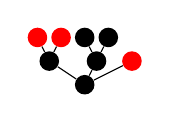
\begin{tikzpicture}[scale=.2]
\node[circle, scale=0.75, fill] (tid0) at (3.75,1.5){};
\node[circle, scale=0.75, fill] (tid1) at (1.5,3){};
\node[circle, scale=0.75, fill, red] (tid4) at (0.75,4.5){};
\node[circle, scale=0.75, fill, red] (tid5) at (2.25,4.5){};
\draw[](tid1) -- (tid4);
\draw[](tid1) -- (tid5);
\node[circle, scale=0.75, fill] (tid2) at (4.5,3){};
\node[circle, scale=0.75, fill] (tid6) at (3.75,4.5){};
\node[circle, scale=0.75, fill] (tid7) at (5.25,4.5){};
\draw[](tid2) -- (tid6);
\draw[](tid2) -- (tid7);
\node[circle, scale=0.75, fill, red] (tid3) at (6.75,3){};
\draw[](tid0) -- (tid1);
\draw[](tid0) -- (tid2);
\draw[](tid0) -- (tid3);
\end{tikzpicture}
\nodepart{two}
\footnotesize{4.64609}
\nodepart{three}
\footnotesize{$67\:33$}
};
 & 
\node[draw=black, rectangle split,  rectangle split parts=3] (sn0x21d54e0){
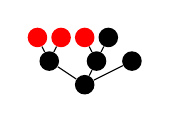
\begin{tikzpicture}[scale=.2]
\node[circle, scale=0.75, fill] (tid0) at (3.75,1.5){};
\node[circle, scale=0.75, fill] (tid1) at (1.5,3){};
\node[circle, scale=0.75, fill, red] (tid4) at (0.75,4.5){};
\node[circle, scale=0.75, fill, red] (tid5) at (2.25,4.5){};
\draw[](tid1) -- (tid4);
\draw[](tid1) -- (tid5);
\node[circle, scale=0.75, fill] (tid2) at (4.5,3){};
\node[circle, scale=0.75, fill, red] (tid6) at (3.75,4.5){};
\node[circle, scale=0.75, fill] (tid7) at (5.25,4.5){};
\draw[](tid2) -- (tid6);
\draw[](tid2) -- (tid7);
\node[circle, scale=0.75, fill] (tid3) at (6.75,3){};
\draw[](tid0) -- (tid1);
\draw[](tid0) -- (tid2);
\draw[](tid0) -- (tid3);
\end{tikzpicture}
\nodepart{two}
\footnotesize{4.57202}
\nodepart{three}
\footnotesize{$17\:50\:33$}
};
 & 
\\
};
\end{scope}
\begin{scope}[yshift=\leveltopIIII cm]
\matrix (line4) [column sep=1cm] {
\node[draw=black, rectangle split,  rectangle split parts=3] (sn0x21ce250){
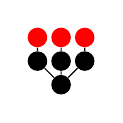
\begin{tikzpicture}[scale=.2]
\node[circle, scale=0.75, fill] (tid0) at (2.25,1.5){};
\node[circle, scale=0.75, fill] (tid1) at (0.75,3){};
\node[circle, scale=0.75, fill, red] (tid4) at (0.75,4.5){};
\draw[](tid1) -- (tid4);
\node[circle, scale=0.75, fill] (tid2) at (2.25,3){};
\node[circle, scale=0.75, fill, red] (tid5) at (2.25,4.5){};
\draw[](tid2) -- (tid5);
\node[circle, scale=0.75, fill] (tid3) at (3.75,3){};
\node[circle, scale=0.75, fill, red] (tid6) at (3.75,4.5){};
\draw[](tid3) -- (tid6);
\draw[](tid0) -- (tid1);
\draw[](tid0) -- (tid2);
\draw[](tid0) -- (tid3);
\end{tikzpicture}
\nodepart{two}
\footnotesize{4.21296}
\nodepart{three}
\footnotesize{$1$}
};
 & 
\node[draw=black, rectangle split,  rectangle split parts=3] (sn0x21d5e10){
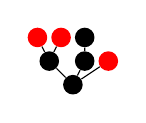
\begin{tikzpicture}[scale=.2]
\node[circle, scale=0.75, fill] (tid0) at (3,1.5){};
\node[circle, scale=0.75, fill] (tid1) at (1.5,3){};
\node[circle, scale=0.75, fill, red] (tid4) at (0.75,4.5){};
\node[circle, scale=0.75, fill, red] (tid5) at (2.25,4.5){};
\draw[](tid1) -- (tid4);
\draw[](tid1) -- (tid5);
\node[circle, scale=0.75, fill] (tid2) at (3.75,3){};
\node[circle, scale=0.75, fill] (tid6) at (3.75,4.5){};
\draw[](tid2) -- (tid6);
\node[circle, scale=0.75, fill, red] (tid3) at (5.25,3){};
\draw[](tid0) -- (tid1);
\draw[](tid0) -- (tid2);
\draw[](tid0) -- (tid3);
\end{tikzpicture}
\nodepart{two}
\footnotesize{4.27161}
\nodepart{three}
\footnotesize{$67\:33$}
};
 & 
\node[draw=black, rectangle split,  rectangle split parts=3] (sn0x21cf5a0){
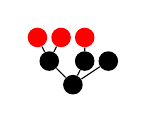
\begin{tikzpicture}[scale=.2]
\node[circle, scale=0.75, fill] (tid0) at (3,1.5){};
\node[circle, scale=0.75, fill] (tid1) at (1.5,3){};
\node[circle, scale=0.75, fill, red] (tid4) at (0.75,4.5){};
\node[circle, scale=0.75, fill, red] (tid5) at (2.25,4.5){};
\draw[](tid1) -- (tid4);
\draw[](tid1) -- (tid5);
\node[circle, scale=0.75, fill] (tid2) at (3.75,3){};
\node[circle, scale=0.75, fill, red] (tid6) at (3.75,4.5){};
\draw[](tid2) -- (tid6);
\node[circle, scale=0.75, fill] (tid3) at (5.25,3){};
\draw[](tid0) -- (tid1);
\draw[](tid0) -- (tid2);
\draw[](tid0) -- (tid3);
\end{tikzpicture}
\nodepart{two}
\footnotesize{4.2037}
\nodepart{three}
\footnotesize{$67\:33$}
};
 & 
\node[draw=black, rectangle split,  rectangle split parts=3] (sn0x21ceae0){
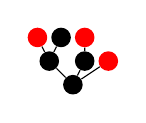
\begin{tikzpicture}[scale=.2]
\node[circle, scale=0.75, fill] (tid0) at (3,1.5){};
\node[circle, scale=0.75, fill] (tid1) at (1.5,3){};
\node[circle, scale=0.75, fill, red] (tid4) at (0.75,4.5){};
\node[circle, scale=0.75, fill] (tid5) at (2.25,4.5){};
\draw[](tid1) -- (tid4);
\draw[](tid1) -- (tid5);
\node[circle, scale=0.75, fill] (tid2) at (3.75,3){};
\node[circle, scale=0.75, fill, red] (tid6) at (3.75,4.5){};
\draw[](tid2) -- (tid6);
\node[circle, scale=0.75, fill, red] (tid3) at (5.25,3){};
\draw[](tid0) -- (tid1);
\draw[](tid0) -- (tid2);
\draw[](tid0) -- (tid3);
\end{tikzpicture}
\nodepart{two}
\footnotesize{4.27469}
\nodepart{three}
\footnotesize{$33\:33\:17\:17$}
};
 & 
\node[draw=black, rectangle split,  rectangle split parts=3] (sn0x21d48e0){
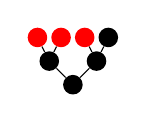
\begin{tikzpicture}[scale=.2]
\node[circle, scale=0.75, fill] (tid0) at (3,1.5){};
\node[circle, scale=0.75, fill] (tid1) at (1.5,3){};
\node[circle, scale=0.75, fill, red] (tid3) at (0.75,4.5){};
\node[circle, scale=0.75, fill, red] (tid4) at (2.25,4.5){};
\draw[](tid1) -- (tid3);
\draw[](tid1) -- (tid4);
\node[circle, scale=0.75, fill] (tid2) at (4.5,3){};
\node[circle, scale=0.75, fill, red] (tid5) at (3.75,4.5){};
\node[circle, scale=0.75, fill] (tid6) at (5.25,4.5){};
\draw[](tid2) -- (tid5);
\draw[](tid2) -- (tid6);
\draw[](tid0) -- (tid1);
\draw[](tid0) -- (tid2);
\end{tikzpicture}
\nodepart{two}
\footnotesize{4.38889}
\nodepart{three}
\footnotesize{$1$}
};
 & 
\\
};
\end{scope}
\begin{scope}[yshift=\leveltopIIIII cm]
\matrix (line5) [column sep=1cm] {
\node[draw=black, rectangle split,  rectangle split parts=3] (sn0x21ced80){
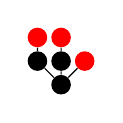
\begin{tikzpicture}[scale=.2]
\node[circle, scale=0.75, fill] (tid0) at (2.25,1.5){};
\node[circle, scale=0.75, fill] (tid1) at (0.75,3){};
\node[circle, scale=0.75, fill, red] (tid4) at (0.75,4.5){};
\draw[](tid1) -- (tid4);
\node[circle, scale=0.75, fill] (tid2) at (2.25,3){};
\node[circle, scale=0.75, fill, red] (tid5) at (2.25,4.5){};
\draw[](tid2) -- (tid5);
\node[circle, scale=0.75, fill, red] (tid3) at (3.75,3){};
\draw[](tid0) -- (tid1);
\draw[](tid0) -- (tid2);
\draw[](tid0) -- (tid3);
\end{tikzpicture}
\nodepart{two}
\footnotesize{3.87963}
\nodepart{three}
\footnotesize{$33\:67$}
};
 & 
\node[draw=black, rectangle split,  rectangle split parts=3] (sn0x21d0e50){
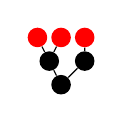
\begin{tikzpicture}[scale=.2]
\node[circle, scale=0.75, fill] (tid0) at (2.25,1.5){};
\node[circle, scale=0.75, fill] (tid1) at (1.5,3){};
\node[circle, scale=0.75, fill, red] (tid3) at (0.75,4.5){};
\node[circle, scale=0.75, fill, red] (tid4) at (2.25,4.5){};
\draw[](tid1) -- (tid3);
\draw[](tid1) -- (tid4);
\node[circle, scale=0.75, fill] (tid2) at (3.75,3){};
\node[circle, scale=0.75, fill, red] (tid5) at (3.75,4.5){};
\draw[](tid2) -- (tid5);
\draw[](tid0) -- (tid1);
\draw[](tid0) -- (tid2);
\end{tikzpicture}
\nodepart{two}
\footnotesize{4.05556}
\nodepart{three}
\footnotesize{$67\:33$}
};
 & 
\node[draw=black, rectangle split,  rectangle split parts=3] (sn0x21d19a0){
\begin{tikzpicture}[scale=.2]
\node[circle, scale=0.75, fill] (tid0) at (3,1.5){};
\node[circle, scale=0.75, fill] (tid1) at (1.5,3){};
\node[circle, scale=0.75, fill, red] (tid4) at (0.75,4.5){};
\node[circle, scale=0.75, fill, red] (tid5) at (2.25,4.5){};
\draw[](tid1) -- (tid4);
\draw[](tid1) -- (tid5);
\node[circle, scale=0.75, fill, red] (tid2) at (3.75,3){};
\node[circle, scale=0.75, fill] (tid3) at (5.25,3){};
\draw[](tid0) -- (tid1);
\draw[](tid0) -- (tid2);
\draw[](tid0) -- (tid3);
\end{tikzpicture}
\nodepart{two}
\footnotesize{3.85185}
\nodepart{three}
\footnotesize{$67\:33$}
};
 & 
\node[draw=black, rectangle split,  rectangle split parts=3] (sn0x21d0fa0){
\begin{tikzpicture}[scale=.2]
\node[circle, scale=0.75, fill] (tid0) at (3,1.5){};
\node[circle, scale=0.75, fill] (tid1) at (1.5,3){};
\node[circle, scale=0.75, fill, red] (tid4) at (0.75,4.5){};
\node[circle, scale=0.75, fill] (tid5) at (2.25,4.5){};
\draw[](tid1) -- (tid4);
\draw[](tid1) -- (tid5);
\node[circle, scale=0.75, fill, red] (tid2) at (3.75,3){};
\node[circle, scale=0.75, fill, red] (tid3) at (5.25,3){};
\draw[](tid0) -- (tid1);
\draw[](tid0) -- (tid2);
\draw[](tid0) -- (tid3);
\end{tikzpicture}
\nodepart{two}
\footnotesize{3.92593}
\nodepart{three}
\footnotesize{$33\:67$}
};
 & 
\\
};
\end{scope}
\begin{scope}[yshift=\leveltopIIIIII cm]
\matrix (line6) [column sep=1cm] {
\node[draw=black, rectangle split,  rectangle split parts=3] (sn0x21cfc10){
\begin{tikzpicture}[scale=.2]
\node[circle, scale=0.75, fill] (tid0) at (1.5,1.5){};
\node[circle, scale=0.75, fill] (tid1) at (0.75,3){};
\node[circle, scale=0.75, fill, red] (tid3) at (0.75,4.5){};
\draw[](tid1) -- (tid3);
\node[circle, scale=0.75, fill] (tid2) at (2.25,3){};
\node[circle, scale=0.75, fill, red] (tid4) at (2.25,4.5){};
\draw[](tid2) -- (tid4);
\draw[](tid0) -- (tid1);
\draw[](tid0) -- (tid2);
\end{tikzpicture}
\nodepart{two}
\footnotesize{3.75}
\nodepart{three}
\footnotesize{$1$}
};
 & 
\node[draw=black, rectangle split,  rectangle split parts=3] (sn0x21cdc20){
\begin{tikzpicture}[scale=.2]
\node[circle, scale=0.75, fill] (tid0) at (2.25,1.5){};
\node[circle, scale=0.75, fill] (tid1) at (0.75,3){};
\node[circle, scale=0.75, fill, red] (tid4) at (0.75,4.5){};
\draw[](tid1) -- (tid4);
\node[circle, scale=0.75, fill, red] (tid2) at (2.25,3){};
\node[circle, scale=0.75, fill, red] (tid3) at (3.75,3){};
\draw[](tid0) -- (tid1);
\draw[](tid0) -- (tid2);
\draw[](tid0) -- (tid3);
\end{tikzpicture}
\nodepart{two}
\footnotesize{3.44444}
\nodepart{three}
\footnotesize{$67\:33$}
};
 & 
\node[draw=black, rectangle split,  rectangle split parts=3] (sn0x21d1cc0){
\begin{tikzpicture}[scale=.2]
\node[circle, scale=0.75, fill] (tid0) at (2.25,1.5){};
\node[circle, scale=0.75, fill] (tid1) at (1.5,3){};
\node[circle, scale=0.75, fill, red] (tid3) at (0.75,4.5){};
\node[circle, scale=0.75, fill, red] (tid4) at (2.25,4.5){};
\draw[](tid1) -- (tid3);
\draw[](tid1) -- (tid4);
\node[circle, scale=0.75, fill, red] (tid2) at (3.75,3){};
\draw[](tid0) -- (tid1);
\draw[](tid0) -- (tid2);
\end{tikzpicture}
\nodepart{two}
\footnotesize{3.66667}
\nodepart{three}
\footnotesize{$67\:33$}
};
 & 
\\
};
\end{scope}
\begin{scope}[yshift=\leveltopIIIIIII cm]
\matrix (line7) [column sep=1cm] {
\node[draw=black, rectangle split,  rectangle split parts=3] (sn0x21cfd50){
\begin{tikzpicture}[scale=.2]
\node[circle, scale=0.75, fill] (tid0) at (1.5,1.5){};
\node[circle, scale=0.75, fill] (tid1) at (0.75,3){};
\node[circle, scale=0.75, fill, red] (tid3) at (0.75,4.5){};
\draw[](tid1) -- (tid3);
\node[circle, scale=0.75, fill, red] (tid2) at (2.25,3){};
\draw[](tid0) -- (tid1);
\draw[](tid0) -- (tid2);
\end{tikzpicture}
\nodepart{two}
\footnotesize{3.25}
\nodepart{three}
\footnotesize{$50\:50$}
};
 & 
\node[draw=black, rectangle split,  rectangle split parts=3] (sn0x21d06a0){
\begin{tikzpicture}[scale=.2]
\node[circle, scale=0.75, fill] (tid0) at (2.25,1.5){};
\node[circle, scale=0.75, fill, red] (tid1) at (0.75,3){};
\node[circle, scale=0.75, fill, red] (tid2) at (2.25,3){};
\node[circle, scale=0.75, fill, red] (tid3) at (3.75,3){};
\draw[](tid0) -- (tid1);
\draw[](tid0) -- (tid2);
\draw[](tid0) -- (tid3);
\end{tikzpicture}
\nodepart{two}
\footnotesize{2.83333}
\nodepart{three}
\footnotesize{$1$}
};
 & 
\node[draw=black, rectangle split,  rectangle split parts=3] (sn0x21d1160){
\begin{tikzpicture}[scale=.2]
\node[circle, scale=0.75, fill] (tid0) at (1.5,1.5){};
\node[circle, scale=0.75, fill] (tid1) at (1.5,3){};
\node[circle, scale=0.75, fill, red] (tid2) at (0.75,4.5){};
\node[circle, scale=0.75, fill, red] (tid3) at (2.25,4.5){};
\draw[](tid1) -- (tid2);
\draw[](tid1) -- (tid3);
\draw[](tid0) -- (tid1);
\end{tikzpicture}
\nodepart{two}
\footnotesize{3.5}
\nodepart{three}
\footnotesize{$1$}
};
 & 
\\
};
\end{scope}
\begin{scope}[yshift=\leveltopIIIIIIII cm]
\matrix (line8) [column sep=1cm] {
\node[draw=black, rectangle split,  rectangle split parts=3] (sn0x21cfe20){
\begin{tikzpicture}[scale=.2]
\node[circle, scale=0.75, fill] (tid0) at (0.75,1.5){};
\node[circle, scale=0.75, fill] (tid1) at (0.75,3){};
\node[circle, scale=0.75, fill, red] (tid2) at (0.75,4.5){};
\draw[](tid1) -- (tid2);
\draw[](tid0) -- (tid1);
\end{tikzpicture}
\nodepart{two}
\footnotesize{3}
\nodepart{three}
\footnotesize{$1$}
};
 & 
\node[draw=black, rectangle split,  rectangle split parts=3] (sn0x21cfef0){
\begin{tikzpicture}[scale=.2]
\node[circle, scale=0.75, fill] (tid0) at (1.5,1.5){};
\node[circle, scale=0.75, fill, red] (tid1) at (0.75,3){};
\node[circle, scale=0.75, fill, red] (tid2) at (2.25,3){};
\draw[](tid0) -- (tid1);
\draw[](tid0) -- (tid2);
\end{tikzpicture}
\nodepart{two}
\footnotesize{2.5}
\nodepart{three}
\footnotesize{$1$}
};
 & 
\\
};
\end{scope}
\begin{scope}[yshift=\leveltopIIIIIIIII cm]
\matrix (line9) [column sep=1cm] {
\node[draw=black, rectangle split,  rectangle split parts=3] (sn0x21cffc0){
\begin{tikzpicture}[scale=.2]
\node[circle, scale=0.75, fill] (tid0) at (0.75,1.5){};
\node[circle, scale=0.75, fill, red] (tid1) at (0.75,3){};
\draw[](tid0) -- (tid1);
\end{tikzpicture}
\nodepart{two}
\footnotesize{2}
\nodepart{three}
\footnotesize{$1$}
};
 & 
\\
};
\end{scope}
\begin{scope}[yshift=\leveltopIIIIIIIIII cm]
\matrix (line10) [column sep=1cm] {
\node[draw=black, rectangle split,  rectangle split parts=3] (sn0x21d0090){
\begin{tikzpicture}[scale=.2]
\node[circle, scale=0.75, fill, red] (tid0) at (0.75,1.5){};
\end{tikzpicture}
\nodepart{two}
\footnotesize{1}
\nodepart{three}
\footnotesize{$$}
};
 & 
\\
};
\end{scope}
\begin{scope}[yshift=\leveltopIIIIIIIIIII cm]
\matrix (line11) [column sep=1cm] {
\\
};
\end{scope}
\draw (sn0x21cb130.south) -- (sn0x21d62b0.north);
\draw (sn0x21cb130.south) -- (sn0x21d6580.north);
\draw (sn0x21d62b0.south) -- (sn0x21d6cd0.north);
\draw (sn0x21d62b0.south) -- (sn0x21ce180.north);
\draw (sn0x21d6580.south) -- (sn0x21ce180.north);
\draw (sn0x21d6580.south) -- (sn0x21d53d0.north);
\draw (sn0x21d6580.south) -- (sn0x21d54e0.north);
\draw (sn0x21d6cd0.south) -- (sn0x21ce250.north);
\draw (sn0x21d6cd0.south) -- (sn0x21d5e10.north);
\draw (sn0x21d6cd0.south) -- (sn0x21cf5a0.north);
\draw (sn0x21ce180.south) -- (sn0x21ce250.north);
\draw (sn0x21ce180.south) -- (sn0x21ceae0.north);
\draw (sn0x21ce180.south) -- (sn0x21cf5a0.north);
\draw (sn0x21d53d0.south) -- (sn0x21d48e0.north);
\draw (sn0x21d53d0.south) -- (sn0x21ceae0.north);
\draw (sn0x21d54e0.south) -- (sn0x21ceae0.north);
\draw (sn0x21d54e0.south) -- (sn0x21cf5a0.north);
\draw (sn0x21d54e0.south) -- (sn0x21d5e10.north);
\draw (sn0x21ce250.south) -- (sn0x21ced80.north);
\draw (sn0x21d5e10.south) -- (sn0x21d0e50.north);
\draw (sn0x21d5e10.south) -- (sn0x21ced80.north);
\draw (sn0x21cf5a0.south) -- (sn0x21ced80.north);
\draw (sn0x21cf5a0.south) -- (sn0x21d19a0.north);
\draw (sn0x21ceae0.south) -- (sn0x21d0e50.north);
\draw (sn0x21ceae0.south) -- (sn0x21ced80.north);
\draw (sn0x21ceae0.south) -- (sn0x21d0fa0.north);
\draw (sn0x21ceae0.south) -- (sn0x21d19a0.north);
\draw (sn0x21d48e0.south) -- (sn0x21d0e50.north);
\draw (sn0x21ced80.south) -- (sn0x21cfc10.north);
\draw (sn0x21ced80.south) -- (sn0x21cdc20.north);
\draw (sn0x21d0e50.south) -- (sn0x21cfc10.north);
\draw (sn0x21d0e50.south) -- (sn0x21d1cc0.north);
\draw (sn0x21d19a0.south) -- (sn0x21d1cc0.north);
\draw (sn0x21d19a0.south) -- (sn0x21cdc20.north);
\draw (sn0x21d0fa0.south) -- (sn0x21d1cc0.north);
\draw (sn0x21d0fa0.south) -- (sn0x21cdc20.north);
\draw (sn0x21cfc10.south) -- (sn0x21cfd50.north);
\draw (sn0x21cdc20.south) -- (sn0x21cfd50.north);
\draw (sn0x21cdc20.south) -- (sn0x21d06a0.north);
\draw (sn0x21d1cc0.south) -- (sn0x21d1160.north);
\draw (sn0x21d1cc0.south) -- (sn0x21cfd50.north);
\draw (sn0x21cfd50.south) -- (sn0x21cfe20.north);
\draw (sn0x21cfd50.south) -- (sn0x21cfef0.north);
\draw (sn0x21d06a0.south) -- (sn0x21cfef0.north);
\draw (sn0x21d1160.south) -- (sn0x21cfe20.north);
\draw (sn0x21cfe20.south) -- (sn0x21cffc0.north);
\draw (sn0x21cfef0.south) -- (sn0x21cffc0.north);
\draw (sn0x21cffc0.south) -- (sn0x21d0090.north);
\end{tikzpicture}

%%% Local Variables:
%%% TeX-master: "thesis/thesis.tex"
%%% End: 
\renewcommand{\leveltopI}{-15cm + \leveltop}
\renewcommand{\leveltopII}{-15cm + \leveltopI}
\renewcommand{\leveltopIII}{-15cm + \leveltopII}
\renewcommand{\leveltopIIII}{-15cm + \leveltopIII}
\renewcommand{\leveltopIIIII}{-15cm + \leveltopIIII}
\renewcommand{\leveltopIIIIII}{-15cm + \leveltopIIIII}
\renewcommand{\leveltopIIIIIII}{-15cm + \leveltopIIIIII}
\renewcommand{\leveltopIIIIIIII}{-15cm + \leveltopIIIIIII}
\renewcommand{\leveltopIIIIIIIII}{-15cm + \leveltopIIIIIIII}
\renewcommand{\leveltopIIIIIIIIII}{-15cm + \leveltopIIIIIIIII}
\begin{tikzpicture}[scale=.2, anchor=south]
\begin{scope}[yshift=\leveltopI cm]
\matrix (line1) [column sep=1cm] {
\node[draw=black, rectangle split,  rectangle split parts=3] (sn0x21cb590){
\begin{tikzpicture}[scale=.2]
\node[circle, scale=0.75, fill] (tid0) at (4.5,1.5){};
\node[circle, scale=0.75, fill] (tid1) at (2.25,3){};
\node[circle, scale=0.75, fill, red] (tid4) at (0.75,4.5){};
\node[circle, scale=0.75, fill, red] (tid5) at (2.25,4.5){};
\node[circle, scale=0.75, fill] (tid6) at (3.75,4.5){};
\draw[](tid1) -- (tid4);
\draw[](tid1) -- (tid5);
\draw[](tid1) -- (tid6);
\node[circle, scale=0.75, fill] (tid2) at (6,3){};
\node[circle, scale=0.75, fill, red] (tid7) at (5.25,4.5){};
\node[circle, scale=0.75, fill] (tid8) at (6.75,4.5){};
\draw[](tid2) -- (tid7);
\draw[](tid2) -- (tid8);
\node[circle, scale=0.75, fill] (tid3) at (8.25,3){};
\node[circle, scale=0.75, fill] (tid9) at (8.25,4.5){};
\draw[](tid3) -- (tid9);
\draw[](tid0) -- (tid1);
\draw[](tid0) -- (tid2);
\draw[](tid0) -- (tid3);
\end{tikzpicture}
\nodepart{two}
\footnotesize{5.2301}
\nodepart{three}
\footnotesize{$44\:22\:11\:22$}
};
 & 
\\
};
\end{scope}
\begin{scope}[yshift=\leveltopII cm]
\matrix (line2) [column sep=1cm] {
\node[draw=black, rectangle split,  rectangle split parts=3] (sn0x21d62b0){
\begin{tikzpicture}[scale=.2]
\node[circle, scale=0.75, fill] (tid0) at (3.75,1.5){};
\node[circle, scale=0.75, fill] (tid1) at (1.5,3){};
\node[circle, scale=0.75, fill, red] (tid4) at (0.75,4.5){};
\node[circle, scale=0.75, fill, red] (tid5) at (2.25,4.5){};
\draw[](tid1) -- (tid4);
\draw[](tid1) -- (tid5);
\node[circle, scale=0.75, fill] (tid2) at (4.5,3){};
\node[circle, scale=0.75, fill, red] (tid6) at (3.75,4.5){};
\node[circle, scale=0.75, fill] (tid7) at (5.25,4.5){};
\draw[](tid2) -- (tid6);
\draw[](tid2) -- (tid7);
\node[circle, scale=0.75, fill] (tid3) at (6.75,3){};
\node[circle, scale=0.75, fill] (tid8) at (6.75,4.5){};
\draw[](tid3) -- (tid8);
\draw[](tid0) -- (tid1);
\draw[](tid0) -- (tid2);
\draw[](tid0) -- (tid3);
\end{tikzpicture}
\nodepart{two}
\footnotesize{4.89095}
\nodepart{three}
\footnotesize{$67\:33$}
};
 & 
\node[draw=black, rectangle split,  rectangle split parts=3] (sn0x21d7190){
\begin{tikzpicture}[scale=.2]
\node[circle, scale=0.75, fill] (tid0) at (3.75,1.5){};
\node[circle, scale=0.75, fill] (tid1) at (1.5,3){};
\node[circle, scale=0.75, fill, red] (tid4) at (0.75,4.5){};
\node[circle, scale=0.75, fill] (tid5) at (2.25,4.5){};
\draw[](tid1) -- (tid4);
\draw[](tid1) -- (tid5);
\node[circle, scale=0.75, fill] (tid2) at (4.5,3){};
\node[circle, scale=0.75, fill, red] (tid6) at (3.75,4.5){};
\node[circle, scale=0.75, fill] (tid7) at (5.25,4.5){};
\draw[](tid2) -- (tid6);
\draw[](tid2) -- (tid7);
\node[circle, scale=0.75, fill] (tid3) at (6.75,3){};
\node[circle, scale=0.75, fill, red] (tid8) at (6.75,4.5){};
\draw[](tid3) -- (tid8);
\draw[](tid0) -- (tid1);
\draw[](tid0) -- (tid2);
\draw[](tid0) -- (tid3);
\end{tikzpicture}
\nodepart{two}
\footnotesize{4.90489}
\nodepart{three}
\footnotesize{$33\:33\:11\:22$}
};
 & 
\node[draw=black, rectangle split,  rectangle split parts=3] (sn0x21d7a90){
\begin{tikzpicture}[scale=.2]
\node[circle, scale=0.75, fill] (tid0) at (3.75,1.5){};
\node[circle, scale=0.75, fill] (tid1) at (2.25,3){};
\node[circle, scale=0.75, fill, red] (tid4) at (0.75,4.5){};
\node[circle, scale=0.75, fill, red] (tid5) at (2.25,4.5){};
\node[circle, scale=0.75, fill, red] (tid6) at (3.75,4.5){};
\draw[](tid1) -- (tid4);
\draw[](tid1) -- (tid5);
\draw[](tid1) -- (tid6);
\node[circle, scale=0.75, fill] (tid2) at (5.25,3){};
\node[circle, scale=0.75, fill] (tid7) at (5.25,4.5){};
\draw[](tid2) -- (tid7);
\node[circle, scale=0.75, fill] (tid3) at (6.75,3){};
\node[circle, scale=0.75, fill] (tid8) at (6.75,4.5){};
\draw[](tid3) -- (tid8);
\draw[](tid0) -- (tid1);
\draw[](tid0) -- (tid2);
\draw[](tid0) -- (tid3);
\end{tikzpicture}
\nodepart{two}
\footnotesize{4.88786}
\nodepart{three}
\footnotesize{$1$}
};
 & 
\node[draw=black, rectangle split,  rectangle split parts=3] (sn0x21d82d0){
\begin{tikzpicture}[scale=.2]
\node[circle, scale=0.75, fill] (tid0) at (3.75,1.5){};
\node[circle, scale=0.75, fill] (tid1) at (2.25,3){};
\node[circle, scale=0.75, fill, red] (tid4) at (0.75,4.5){};
\node[circle, scale=0.75, fill, red] (tid5) at (2.25,4.5){};
\node[circle, scale=0.75, fill] (tid6) at (3.75,4.5){};
\draw[](tid1) -- (tid4);
\draw[](tid1) -- (tid5);
\draw[](tid1) -- (tid6);
\node[circle, scale=0.75, fill] (tid2) at (5.25,3){};
\node[circle, scale=0.75, fill, red] (tid7) at (5.25,4.5){};
\draw[](tid2) -- (tid7);
\node[circle, scale=0.75, fill] (tid3) at (6.75,3){};
\node[circle, scale=0.75, fill] (tid8) at (6.75,4.5){};
\draw[](tid3) -- (tid8);
\draw[](tid0) -- (tid1);
\draw[](tid0) -- (tid2);
\draw[](tid0) -- (tid3);
\end{tikzpicture}
\nodepart{two}
\footnotesize{4.90472}
\nodepart{three}
\footnotesize{$33\:33\:11\:11\:11$}
};
 & 
\\
};
\end{scope}
\begin{scope}[yshift=\leveltopIII cm]
\matrix (line3) [column sep=1cm] {
\node[draw=black, rectangle split,  rectangle split parts=3] (sn0x21d6cd0){
\begin{tikzpicture}[scale=.2]
\node[circle, scale=0.75, fill] (tid0) at (3,1.5){};
\node[circle, scale=0.75, fill] (tid1) at (1.5,3){};
\node[circle, scale=0.75, fill, red] (tid4) at (0.75,4.5){};
\node[circle, scale=0.75, fill, red] (tid5) at (2.25,4.5){};
\draw[](tid1) -- (tid4);
\draw[](tid1) -- (tid5);
\node[circle, scale=0.75, fill] (tid2) at (3.75,3){};
\node[circle, scale=0.75, fill, red] (tid6) at (3.75,4.5){};
\draw[](tid2) -- (tid6);
\node[circle, scale=0.75, fill] (tid3) at (5.25,3){};
\node[circle, scale=0.75, fill] (tid7) at (5.25,4.5){};
\draw[](tid3) -- (tid7);
\draw[](tid0) -- (tid1);
\draw[](tid0) -- (tid2);
\draw[](tid0) -- (tid3);
\end{tikzpicture}
\nodepart{two}
\footnotesize{4.55453}
\nodepart{three}
\footnotesize{$67\:17\:17$}
};
 & 
\node[draw=black, rectangle split,  rectangle split parts=3] (sn0x21ce180){
\begin{tikzpicture}[scale=.2]
\node[circle, scale=0.75, fill] (tid0) at (3,1.5){};
\node[circle, scale=0.75, fill] (tid1) at (1.5,3){};
\node[circle, scale=0.75, fill, red] (tid4) at (0.75,4.5){};
\node[circle, scale=0.75, fill] (tid5) at (2.25,4.5){};
\draw[](tid1) -- (tid4);
\draw[](tid1) -- (tid5);
\node[circle, scale=0.75, fill] (tid2) at (3.75,3){};
\node[circle, scale=0.75, fill, red] (tid6) at (3.75,4.5){};
\draw[](tid2) -- (tid6);
\node[circle, scale=0.75, fill] (tid3) at (5.25,3){};
\node[circle, scale=0.75, fill, red] (tid7) at (5.25,4.5){};
\draw[](tid3) -- (tid7);
\draw[](tid0) -- (tid1);
\draw[](tid0) -- (tid2);
\draw[](tid0) -- (tid3);
\end{tikzpicture}
\nodepart{two}
\footnotesize{4.56379}
\nodepart{three}
\footnotesize{$33\:33\:33$}
};
 & 
\node[draw=black, rectangle split,  rectangle split parts=3] (sn0x21d7c90){
\begin{tikzpicture}[scale=.2]
\node[circle, scale=0.75, fill] (tid0) at (3.75,1.5){};
\node[circle, scale=0.75, fill] (tid1) at (1.5,3){};
\node[circle, scale=0.75, fill, red] (tid4) at (0.75,4.5){};
\node[circle, scale=0.75, fill] (tid5) at (2.25,4.5){};
\draw[](tid1) -- (tid4);
\draw[](tid1) -- (tid5);
\node[circle, scale=0.75, fill] (tid2) at (4.5,3){};
\node[circle, scale=0.75, fill, red] (tid6) at (3.75,4.5){};
\node[circle, scale=0.75, fill] (tid7) at (5.25,4.5){};
\draw[](tid2) -- (tid6);
\draw[](tid2) -- (tid7);
\node[circle, scale=0.75, fill, red] (tid3) at (6.75,3){};
\draw[](tid0) -- (tid1);
\draw[](tid0) -- (tid2);
\draw[](tid0) -- (tid3);
\end{tikzpicture}
\nodepart{two}
\footnotesize{4.64506}
\nodepart{three}
\footnotesize{$33\:33\:33$}
};
 & 
\node[draw=black, rectangle split,  rectangle split parts=3] (sn0x21d54e0){
\begin{tikzpicture}[scale=.2]
\node[circle, scale=0.75, fill] (tid0) at (3.75,1.5){};
\node[circle, scale=0.75, fill] (tid1) at (1.5,3){};
\node[circle, scale=0.75, fill, red] (tid4) at (0.75,4.5){};
\node[circle, scale=0.75, fill, red] (tid5) at (2.25,4.5){};
\draw[](tid1) -- (tid4);
\draw[](tid1) -- (tid5);
\node[circle, scale=0.75, fill] (tid2) at (4.5,3){};
\node[circle, scale=0.75, fill, red] (tid6) at (3.75,4.5){};
\node[circle, scale=0.75, fill] (tid7) at (5.25,4.5){};
\draw[](tid2) -- (tid6);
\draw[](tid2) -- (tid7);
\node[circle, scale=0.75, fill] (tid3) at (6.75,3){};
\draw[](tid0) -- (tid1);
\draw[](tid0) -- (tid2);
\draw[](tid0) -- (tid3);
\end{tikzpicture}
\nodepart{two}
\footnotesize{4.57202}
\nodepart{three}
\footnotesize{$17\:50\:33$}
};
 & 
\node[draw=black, rectangle split,  rectangle split parts=3] (sn0x21d8700){
\begin{tikzpicture}[scale=.2]
\node[circle, scale=0.75, fill] (tid0) at (3.75,1.5){};
\node[circle, scale=0.75, fill] (tid1) at (2.25,3){};
\node[circle, scale=0.75, fill, red] (tid4) at (0.75,4.5){};
\node[circle, scale=0.75, fill, red] (tid5) at (2.25,4.5){};
\node[circle, scale=0.75, fill] (tid6) at (3.75,4.5){};
\draw[](tid1) -- (tid4);
\draw[](tid1) -- (tid5);
\draw[](tid1) -- (tid6);
\node[circle, scale=0.75, fill] (tid2) at (5.25,3){};
\node[circle, scale=0.75, fill] (tid7) at (5.25,4.5){};
\draw[](tid2) -- (tid7);
\node[circle, scale=0.75, fill, red] (tid3) at (6.75,3){};
\draw[](tid0) -- (tid1);
\draw[](tid0) -- (tid2);
\draw[](tid0) -- (tid3);
\end{tikzpicture}
\nodepart{two}
\footnotesize{4.64352}
\nodepart{three}
\footnotesize{$33\:33\:17\:17$}
};
 & 
\node[draw=black, rectangle split,  rectangle split parts=3] (sn0x21d8820){
\begin{tikzpicture}[scale=.2]
\node[circle, scale=0.75, fill] (tid0) at (3.75,1.5){};
\node[circle, scale=0.75, fill] (tid1) at (2.25,3){};
\node[circle, scale=0.75, fill, red] (tid4) at (0.75,4.5){};
\node[circle, scale=0.75, fill, red] (tid5) at (2.25,4.5){};
\node[circle, scale=0.75, fill, red] (tid6) at (3.75,4.5){};
\draw[](tid1) -- (tid4);
\draw[](tid1) -- (tid5);
\draw[](tid1) -- (tid6);
\node[circle, scale=0.75, fill] (tid2) at (5.25,3){};
\node[circle, scale=0.75, fill] (tid7) at (5.25,4.5){};
\draw[](tid2) -- (tid7);
\node[circle, scale=0.75, fill] (tid3) at (6.75,3){};
\draw[](tid0) -- (tid1);
\draw[](tid0) -- (tid2);
\draw[](tid0) -- (tid3);
\end{tikzpicture}
\nodepart{two}
\footnotesize{4.57099}
\nodepart{three}
\footnotesize{$50\:50$}
};
 & 
\node[draw=black, rectangle split,  rectangle split parts=3] (sn0x21ce760){
\begin{tikzpicture}[scale=.2]
\node[circle, scale=0.75, fill] (tid0) at (3.75,1.5){};
\node[circle, scale=0.75, fill] (tid1) at (2.25,3){};
\node[circle, scale=0.75, fill, red] (tid4) at (0.75,4.5){};
\node[circle, scale=0.75, fill, red] (tid5) at (2.25,4.5){};
\node[circle, scale=0.75, fill] (tid6) at (3.75,4.5){};
\draw[](tid1) -- (tid4);
\draw[](tid1) -- (tid5);
\draw[](tid1) -- (tid6);
\node[circle, scale=0.75, fill] (tid2) at (5.25,3){};
\node[circle, scale=0.75, fill, red] (tid7) at (5.25,4.5){};
\draw[](tid2) -- (tid7);
\node[circle, scale=0.75, fill] (tid3) at (6.75,3){};
\draw[](tid0) -- (tid1);
\draw[](tid0) -- (tid2);
\draw[](tid0) -- (tid3);
\end{tikzpicture}
\nodepart{two}
\footnotesize{4.57305}
\nodepart{three}
\footnotesize{$33\:33\:22\:11$}
};
 & 
\\
};
\end{scope}
\begin{scope}[yshift=\leveltopIIII cm]
\matrix (line4) [column sep=1cm] {
\node[draw=black, rectangle split,  rectangle split parts=3] (sn0x21ce250){
\begin{tikzpicture}[scale=.2]
\node[circle, scale=0.75, fill] (tid0) at (2.25,1.5){};
\node[circle, scale=0.75, fill] (tid1) at (0.75,3){};
\node[circle, scale=0.75, fill, red] (tid4) at (0.75,4.5){};
\draw[](tid1) -- (tid4);
\node[circle, scale=0.75, fill] (tid2) at (2.25,3){};
\node[circle, scale=0.75, fill, red] (tid5) at (2.25,4.5){};
\draw[](tid2) -- (tid5);
\node[circle, scale=0.75, fill] (tid3) at (3.75,3){};
\node[circle, scale=0.75, fill, red] (tid6) at (3.75,4.5){};
\draw[](tid3) -- (tid6);
\draw[](tid0) -- (tid1);
\draw[](tid0) -- (tid2);
\draw[](tid0) -- (tid3);
\end{tikzpicture}
\nodepart{two}
\footnotesize{4.21296}
\nodepart{three}
\footnotesize{$1$}
};
 & 
\node[draw=black, rectangle split,  rectangle split parts=3] (sn0x21d5e10){
\begin{tikzpicture}[scale=.2]
\node[circle, scale=0.75, fill] (tid0) at (3,1.5){};
\node[circle, scale=0.75, fill] (tid1) at (1.5,3){};
\node[circle, scale=0.75, fill, red] (tid4) at (0.75,4.5){};
\node[circle, scale=0.75, fill, red] (tid5) at (2.25,4.5){};
\draw[](tid1) -- (tid4);
\draw[](tid1) -- (tid5);
\node[circle, scale=0.75, fill] (tid2) at (3.75,3){};
\node[circle, scale=0.75, fill] (tid6) at (3.75,4.5){};
\draw[](tid2) -- (tid6);
\node[circle, scale=0.75, fill, red] (tid3) at (5.25,3){};
\draw[](tid0) -- (tid1);
\draw[](tid0) -- (tid2);
\draw[](tid0) -- (tid3);
\end{tikzpicture}
\nodepart{two}
\footnotesize{4.27161}
\nodepart{three}
\footnotesize{$67\:33$}
};
 & 
\node[draw=black, rectangle split,  rectangle split parts=3] (sn0x21cf5a0){
\begin{tikzpicture}[scale=.2]
\node[circle, scale=0.75, fill] (tid0) at (3,1.5){};
\node[circle, scale=0.75, fill] (tid1) at (1.5,3){};
\node[circle, scale=0.75, fill, red] (tid4) at (0.75,4.5){};
\node[circle, scale=0.75, fill, red] (tid5) at (2.25,4.5){};
\draw[](tid1) -- (tid4);
\draw[](tid1) -- (tid5);
\node[circle, scale=0.75, fill] (tid2) at (3.75,3){};
\node[circle, scale=0.75, fill, red] (tid6) at (3.75,4.5){};
\draw[](tid2) -- (tid6);
\node[circle, scale=0.75, fill] (tid3) at (5.25,3){};
\draw[](tid0) -- (tid1);
\draw[](tid0) -- (tid2);
\draw[](tid0) -- (tid3);
\end{tikzpicture}
\nodepart{two}
\footnotesize{4.2037}
\nodepart{three}
\footnotesize{$67\:33$}
};
 & 
\node[draw=black, rectangle split,  rectangle split parts=3] (sn0x21ceae0){
\begin{tikzpicture}[scale=.2]
\node[circle, scale=0.75, fill] (tid0) at (3,1.5){};
\node[circle, scale=0.75, fill] (tid1) at (1.5,3){};
\node[circle, scale=0.75, fill, red] (tid4) at (0.75,4.5){};
\node[circle, scale=0.75, fill] (tid5) at (2.25,4.5){};
\draw[](tid1) -- (tid4);
\draw[](tid1) -- (tid5);
\node[circle, scale=0.75, fill] (tid2) at (3.75,3){};
\node[circle, scale=0.75, fill, red] (tid6) at (3.75,4.5){};
\draw[](tid2) -- (tid6);
\node[circle, scale=0.75, fill, red] (tid3) at (5.25,3){};
\draw[](tid0) -- (tid1);
\draw[](tid0) -- (tid2);
\draw[](tid0) -- (tid3);
\end{tikzpicture}
\nodepart{two}
\footnotesize{4.27469}
\nodepart{three}
\footnotesize{$33\:33\:17\:17$}
};
 & 
\node[draw=black, rectangle split,  rectangle split parts=3] (sn0x21d48e0){
\begin{tikzpicture}[scale=.2]
\node[circle, scale=0.75, fill] (tid0) at (3,1.5){};
\node[circle, scale=0.75, fill] (tid1) at (1.5,3){};
\node[circle, scale=0.75, fill, red] (tid3) at (0.75,4.5){};
\node[circle, scale=0.75, fill, red] (tid4) at (2.25,4.5){};
\draw[](tid1) -- (tid3);
\draw[](tid1) -- (tid4);
\node[circle, scale=0.75, fill] (tid2) at (4.5,3){};
\node[circle, scale=0.75, fill, red] (tid5) at (3.75,4.5){};
\node[circle, scale=0.75, fill] (tid6) at (5.25,4.5){};
\draw[](tid2) -- (tid5);
\draw[](tid2) -- (tid6);
\draw[](tid0) -- (tid1);
\draw[](tid0) -- (tid2);
\end{tikzpicture}
\nodepart{two}
\footnotesize{4.38889}
\nodepart{three}
\footnotesize{$1$}
};
 & 
\node[draw=black, rectangle split,  rectangle split parts=3] (sn0x21d9480){
\begin{tikzpicture}[scale=.2]
\node[circle, scale=0.75, fill] (tid0) at (3,1.5){};
\node[circle, scale=0.75, fill] (tid1) at (2.25,3){};
\node[circle, scale=0.75, fill, red] (tid3) at (0.75,4.5){};
\node[circle, scale=0.75, fill, red] (tid4) at (2.25,4.5){};
\node[circle, scale=0.75, fill, red] (tid5) at (3.75,4.5){};
\draw[](tid1) -- (tid3);
\draw[](tid1) -- (tid4);
\draw[](tid1) -- (tid5);
\node[circle, scale=0.75, fill] (tid2) at (5.25,3){};
\node[circle, scale=0.75, fill] (tid6) at (5.25,4.5){};
\draw[](tid2) -- (tid6);
\draw[](tid0) -- (tid1);
\draw[](tid0) -- (tid2);
\end{tikzpicture}
\nodepart{two}
\footnotesize{4.38889}
\nodepart{three}
\footnotesize{$1$}
};
 & 
\node[draw=black, rectangle split,  rectangle split parts=3] (sn0x21d22d0){
\begin{tikzpicture}[scale=.2]
\node[circle, scale=0.75, fill] (tid0) at (3,1.5){};
\node[circle, scale=0.75, fill] (tid1) at (2.25,3){};
\node[circle, scale=0.75, fill, red] (tid3) at (0.75,4.5){};
\node[circle, scale=0.75, fill, red] (tid4) at (2.25,4.5){};
\node[circle, scale=0.75, fill] (tid5) at (3.75,4.5){};
\draw[](tid1) -- (tid3);
\draw[](tid1) -- (tid4);
\draw[](tid1) -- (tid5);
\node[circle, scale=0.75, fill] (tid2) at (5.25,3){};
\node[circle, scale=0.75, fill, red] (tid6) at (5.25,4.5){};
\draw[](tid2) -- (tid6);
\draw[](tid0) -- (tid1);
\draw[](tid0) -- (tid2);
\end{tikzpicture}
\nodepart{two}
\footnotesize{4.37963}
\nodepart{three}
\footnotesize{$67\:17\:17$}
};
 & 
\node[draw=black, rectangle split,  rectangle split parts=3] (sn0x21d3130){
\begin{tikzpicture}[scale=.2]
\node[circle, scale=0.75, fill] (tid0) at (3.75,1.5){};
\node[circle, scale=0.75, fill] (tid1) at (2.25,3){};
\node[circle, scale=0.75, fill, red] (tid4) at (0.75,4.5){};
\node[circle, scale=0.75, fill, red] (tid5) at (2.25,4.5){};
\node[circle, scale=0.75, fill] (tid6) at (3.75,4.5){};
\draw[](tid1) -- (tid4);
\draw[](tid1) -- (tid5);
\draw[](tid1) -- (tid6);
\node[circle, scale=0.75, fill, red] (tid2) at (5.25,3){};
\node[circle, scale=0.75, fill] (tid3) at (6.75,3){};
\draw[](tid0) -- (tid1);
\draw[](tid0) -- (tid2);
\draw[](tid0) -- (tid3);
\end{tikzpicture}
\nodepart{two}
\footnotesize{4.26852}
\nodepart{three}
\footnotesize{$33\:33\:17\:17$}
};
 & 
\node[draw=black, rectangle split,  rectangle split parts=3] (sn0x21d4280){
\begin{tikzpicture}[scale=.2]
\node[circle, scale=0.75, fill] (tid0) at (3.75,1.5){};
\node[circle, scale=0.75, fill] (tid1) at (2.25,3){};
\node[circle, scale=0.75, fill, red] (tid4) at (0.75,4.5){};
\node[circle, scale=0.75, fill, red] (tid5) at (2.25,4.5){};
\node[circle, scale=0.75, fill, red] (tid6) at (3.75,4.5){};
\draw[](tid1) -- (tid4);
\draw[](tid1) -- (tid5);
\draw[](tid1) -- (tid6);
\node[circle, scale=0.75, fill] (tid2) at (5.25,3){};
\node[circle, scale=0.75, fill] (tid3) at (6.75,3){};
\draw[](tid0) -- (tid1);
\draw[](tid0) -- (tid2);
\draw[](tid0) -- (tid3);
\end{tikzpicture}
\nodepart{two}
\footnotesize{4.18519}
\nodepart{three}
\footnotesize{$1$}
};
 & 
\\
};
\end{scope}
\begin{scope}[yshift=\leveltopIIIII cm]
\matrix (line5) [column sep=1cm] {
\node[draw=black, rectangle split,  rectangle split parts=3] (sn0x21ced80){
\begin{tikzpicture}[scale=.2]
\node[circle, scale=0.75, fill] (tid0) at (2.25,1.5){};
\node[circle, scale=0.75, fill] (tid1) at (0.75,3){};
\node[circle, scale=0.75, fill, red] (tid4) at (0.75,4.5){};
\draw[](tid1) -- (tid4);
\node[circle, scale=0.75, fill] (tid2) at (2.25,3){};
\node[circle, scale=0.75, fill, red] (tid5) at (2.25,4.5){};
\draw[](tid2) -- (tid5);
\node[circle, scale=0.75, fill, red] (tid3) at (3.75,3){};
\draw[](tid0) -- (tid1);
\draw[](tid0) -- (tid2);
\draw[](tid0) -- (tid3);
\end{tikzpicture}
\nodepart{two}
\footnotesize{3.87963}
\nodepart{three}
\footnotesize{$33\:67$}
};
 & 
\node[draw=black, rectangle split,  rectangle split parts=3] (sn0x21d0e50){
\begin{tikzpicture}[scale=.2]
\node[circle, scale=0.75, fill] (tid0) at (2.25,1.5){};
\node[circle, scale=0.75, fill] (tid1) at (1.5,3){};
\node[circle, scale=0.75, fill, red] (tid3) at (0.75,4.5){};
\node[circle, scale=0.75, fill, red] (tid4) at (2.25,4.5){};
\draw[](tid1) -- (tid3);
\draw[](tid1) -- (tid4);
\node[circle, scale=0.75, fill] (tid2) at (3.75,3){};
\node[circle, scale=0.75, fill, red] (tid5) at (3.75,4.5){};
\draw[](tid2) -- (tid5);
\draw[](tid0) -- (tid1);
\draw[](tid0) -- (tid2);
\end{tikzpicture}
\nodepart{two}
\footnotesize{4.05556}
\nodepart{three}
\footnotesize{$67\:33$}
};
 & 
\node[draw=black, rectangle split,  rectangle split parts=3] (sn0x21d19a0){
\begin{tikzpicture}[scale=.2]
\node[circle, scale=0.75, fill] (tid0) at (3,1.5){};
\node[circle, scale=0.75, fill] (tid1) at (1.5,3){};
\node[circle, scale=0.75, fill, red] (tid4) at (0.75,4.5){};
\node[circle, scale=0.75, fill, red] (tid5) at (2.25,4.5){};
\draw[](tid1) -- (tid4);
\draw[](tid1) -- (tid5);
\node[circle, scale=0.75, fill, red] (tid2) at (3.75,3){};
\node[circle, scale=0.75, fill] (tid3) at (5.25,3){};
\draw[](tid0) -- (tid1);
\draw[](tid0) -- (tid2);
\draw[](tid0) -- (tid3);
\end{tikzpicture}
\nodepart{two}
\footnotesize{3.85185}
\nodepart{three}
\footnotesize{$67\:33$}
};
 & 
\node[draw=black, rectangle split,  rectangle split parts=3] (sn0x21d0fa0){
\begin{tikzpicture}[scale=.2]
\node[circle, scale=0.75, fill] (tid0) at (3,1.5){};
\node[circle, scale=0.75, fill] (tid1) at (1.5,3){};
\node[circle, scale=0.75, fill, red] (tid4) at (0.75,4.5){};
\node[circle, scale=0.75, fill] (tid5) at (2.25,4.5){};
\draw[](tid1) -- (tid4);
\draw[](tid1) -- (tid5);
\node[circle, scale=0.75, fill, red] (tid2) at (3.75,3){};
\node[circle, scale=0.75, fill, red] (tid3) at (5.25,3){};
\draw[](tid0) -- (tid1);
\draw[](tid0) -- (tid2);
\draw[](tid0) -- (tid3);
\end{tikzpicture}
\nodepart{two}
\footnotesize{3.92593}
\nodepart{three}
\footnotesize{$33\:67$}
};
 & 
\node[draw=black, rectangle split,  rectangle split parts=3] (sn0x21d36b0){
\begin{tikzpicture}[scale=.2]
\node[circle, scale=0.75, fill] (tid0) at (3,1.5){};
\node[circle, scale=0.75, fill] (tid1) at (2.25,3){};
\node[circle, scale=0.75, fill, red] (tid3) at (0.75,4.5){};
\node[circle, scale=0.75, fill, red] (tid4) at (2.25,4.5){};
\node[circle, scale=0.75, fill] (tid5) at (3.75,4.5){};
\draw[](tid1) -- (tid3);
\draw[](tid1) -- (tid4);
\draw[](tid1) -- (tid5);
\node[circle, scale=0.75, fill, red] (tid2) at (5.25,3){};
\draw[](tid0) -- (tid1);
\draw[](tid0) -- (tid2);
\end{tikzpicture}
\nodepart{two}
\footnotesize{4.05556}
\nodepart{three}
\footnotesize{$67\:33$}
};
 & 
\node[draw=black, rectangle split,  rectangle split parts=3] (sn0x21d34d0){
\begin{tikzpicture}[scale=.2]
\node[circle, scale=0.75, fill] (tid0) at (3,1.5){};
\node[circle, scale=0.75, fill] (tid1) at (2.25,3){};
\node[circle, scale=0.75, fill, red] (tid3) at (0.75,4.5){};
\node[circle, scale=0.75, fill, red] (tid4) at (2.25,4.5){};
\node[circle, scale=0.75, fill, red] (tid5) at (3.75,4.5){};
\draw[](tid1) -- (tid3);
\draw[](tid1) -- (tid4);
\draw[](tid1) -- (tid5);
\node[circle, scale=0.75, fill] (tid2) at (5.25,3){};
\draw[](tid0) -- (tid1);
\draw[](tid0) -- (tid2);
\end{tikzpicture}
\nodepart{two}
\footnotesize{4}
\nodepart{three}
\footnotesize{$1$}
};
 & 
\\
};
\end{scope}
\begin{scope}[yshift=\leveltopIIIIII cm]
\matrix (line6) [column sep=1cm] {
\node[draw=black, rectangle split,  rectangle split parts=3] (sn0x21cfc10){
\begin{tikzpicture}[scale=.2]
\node[circle, scale=0.75, fill] (tid0) at (1.5,1.5){};
\node[circle, scale=0.75, fill] (tid1) at (0.75,3){};
\node[circle, scale=0.75, fill, red] (tid3) at (0.75,4.5){};
\draw[](tid1) -- (tid3);
\node[circle, scale=0.75, fill] (tid2) at (2.25,3){};
\node[circle, scale=0.75, fill, red] (tid4) at (2.25,4.5){};
\draw[](tid2) -- (tid4);
\draw[](tid0) -- (tid1);
\draw[](tid0) -- (tid2);
\end{tikzpicture}
\nodepart{two}
\footnotesize{3.75}
\nodepart{three}
\footnotesize{$1$}
};
 & 
\node[draw=black, rectangle split,  rectangle split parts=3] (sn0x21cdc20){
\begin{tikzpicture}[scale=.2]
\node[circle, scale=0.75, fill] (tid0) at (2.25,1.5){};
\node[circle, scale=0.75, fill] (tid1) at (0.75,3){};
\node[circle, scale=0.75, fill, red] (tid4) at (0.75,4.5){};
\draw[](tid1) -- (tid4);
\node[circle, scale=0.75, fill, red] (tid2) at (2.25,3){};
\node[circle, scale=0.75, fill, red] (tid3) at (3.75,3){};
\draw[](tid0) -- (tid1);
\draw[](tid0) -- (tid2);
\draw[](tid0) -- (tid3);
\end{tikzpicture}
\nodepart{two}
\footnotesize{3.44444}
\nodepart{three}
\footnotesize{$67\:33$}
};
 & 
\node[draw=black, rectangle split,  rectangle split parts=3] (sn0x21d1cc0){
\begin{tikzpicture}[scale=.2]
\node[circle, scale=0.75, fill] (tid0) at (2.25,1.5){};
\node[circle, scale=0.75, fill] (tid1) at (1.5,3){};
\node[circle, scale=0.75, fill, red] (tid3) at (0.75,4.5){};
\node[circle, scale=0.75, fill, red] (tid4) at (2.25,4.5){};
\draw[](tid1) -- (tid3);
\draw[](tid1) -- (tid4);
\node[circle, scale=0.75, fill, red] (tid2) at (3.75,3){};
\draw[](tid0) -- (tid1);
\draw[](tid0) -- (tid2);
\end{tikzpicture}
\nodepart{two}
\footnotesize{3.66667}
\nodepart{three}
\footnotesize{$67\:33$}
};
 & 
\node[draw=black, rectangle split,  rectangle split parts=3] (sn0x21d3bb0){
\begin{tikzpicture}[scale=.2]
\node[circle, scale=0.75, fill] (tid0) at (2.25,1.5){};
\node[circle, scale=0.75, fill] (tid1) at (2.25,3){};
\node[circle, scale=0.75, fill, red] (tid2) at (0.75,4.5){};
\node[circle, scale=0.75, fill, red] (tid3) at (2.25,4.5){};
\node[circle, scale=0.75, fill, red] (tid4) at (3.75,4.5){};
\draw[](tid1) -- (tid2);
\draw[](tid1) -- (tid3);
\draw[](tid1) -- (tid4);
\draw[](tid0) -- (tid1);
\end{tikzpicture}
\nodepart{two}
\footnotesize{3.83333}
\nodepart{three}
\footnotesize{$1$}
};
 & 
\\
};
\end{scope}
\begin{scope}[yshift=\leveltopIIIIIII cm]
\matrix (line7) [column sep=1cm] {
\node[draw=black, rectangle split,  rectangle split parts=3] (sn0x21cfd50){
\begin{tikzpicture}[scale=.2]
\node[circle, scale=0.75, fill] (tid0) at (1.5,1.5){};
\node[circle, scale=0.75, fill] (tid1) at (0.75,3){};
\node[circle, scale=0.75, fill, red] (tid3) at (0.75,4.5){};
\draw[](tid1) -- (tid3);
\node[circle, scale=0.75, fill, red] (tid2) at (2.25,3){};
\draw[](tid0) -- (tid1);
\draw[](tid0) -- (tid2);
\end{tikzpicture}
\nodepart{two}
\footnotesize{3.25}
\nodepart{three}
\footnotesize{$50\:50$}
};
 & 
\node[draw=black, rectangle split,  rectangle split parts=3] (sn0x21d06a0){
\begin{tikzpicture}[scale=.2]
\node[circle, scale=0.75, fill] (tid0) at (2.25,1.5){};
\node[circle, scale=0.75, fill, red] (tid1) at (0.75,3){};
\node[circle, scale=0.75, fill, red] (tid2) at (2.25,3){};
\node[circle, scale=0.75, fill, red] (tid3) at (3.75,3){};
\draw[](tid0) -- (tid1);
\draw[](tid0) -- (tid2);
\draw[](tid0) -- (tid3);
\end{tikzpicture}
\nodepart{two}
\footnotesize{2.83333}
\nodepart{three}
\footnotesize{$1$}
};
 & 
\node[draw=black, rectangle split,  rectangle split parts=3] (sn0x21d1160){
\begin{tikzpicture}[scale=.2]
\node[circle, scale=0.75, fill] (tid0) at (1.5,1.5){};
\node[circle, scale=0.75, fill] (tid1) at (1.5,3){};
\node[circle, scale=0.75, fill, red] (tid2) at (0.75,4.5){};
\node[circle, scale=0.75, fill, red] (tid3) at (2.25,4.5){};
\draw[](tid1) -- (tid2);
\draw[](tid1) -- (tid3);
\draw[](tid0) -- (tid1);
\end{tikzpicture}
\nodepart{two}
\footnotesize{3.5}
\nodepart{three}
\footnotesize{$1$}
};
 & 
\\
};
\end{scope}
\begin{scope}[yshift=\leveltopIIIIIIII cm]
\matrix (line8) [column sep=1cm] {
\node[draw=black, rectangle split,  rectangle split parts=3] (sn0x21cfe20){
\begin{tikzpicture}[scale=.2]
\node[circle, scale=0.75, fill] (tid0) at (0.75,1.5){};
\node[circle, scale=0.75, fill] (tid1) at (0.75,3){};
\node[circle, scale=0.75, fill, red] (tid2) at (0.75,4.5){};
\draw[](tid1) -- (tid2);
\draw[](tid0) -- (tid1);
\end{tikzpicture}
\nodepart{two}
\footnotesize{3}
\nodepart{three}
\footnotesize{$1$}
};
 & 
\node[draw=black, rectangle split,  rectangle split parts=3] (sn0x21cfef0){
\begin{tikzpicture}[scale=.2]
\node[circle, scale=0.75, fill] (tid0) at (1.5,1.5){};
\node[circle, scale=0.75, fill, red] (tid1) at (0.75,3){};
\node[circle, scale=0.75, fill, red] (tid2) at (2.25,3){};
\draw[](tid0) -- (tid1);
\draw[](tid0) -- (tid2);
\end{tikzpicture}
\nodepart{two}
\footnotesize{2.5}
\nodepart{three}
\footnotesize{$1$}
};
 & 
\\
};
\end{scope}
\begin{scope}[yshift=\leveltopIIIIIIIII cm]
\matrix (line9) [column sep=1cm] {
\node[draw=black, rectangle split,  rectangle split parts=3] (sn0x21cffc0){
\begin{tikzpicture}[scale=.2]
\node[circle, scale=0.75, fill] (tid0) at (0.75,1.5){};
\node[circle, scale=0.75, fill, red] (tid1) at (0.75,3){};
\draw[](tid0) -- (tid1);
\end{tikzpicture}
\nodepart{two}
\footnotesize{2}
\nodepart{three}
\footnotesize{$1$}
};
 & 
\\
};
\end{scope}
\begin{scope}[yshift=\leveltopIIIIIIIIII cm]
\matrix (line10) [column sep=1cm] {
\node[draw=black, rectangle split,  rectangle split parts=3] (sn0x21d0090){
\begin{tikzpicture}[scale=.2]
\node[circle, scale=0.75, fill, red] (tid0) at (0.75,1.5){};
\end{tikzpicture}
\nodepart{two}
\footnotesize{1}
\nodepart{three}
\footnotesize{$$}
};
 & 
\\
};
\end{scope}
\begin{scope}[yshift=\leveltopIIIIIIIIIII cm]
\matrix (line11) [column sep=1cm] {
\\
};
\end{scope}
\draw (sn0x21cb590.south) -- (sn0x21d62b0.north);
\draw (sn0x21cb590.south) -- (sn0x21d7190.north);
\draw (sn0x21cb590.south) -- (sn0x21d7a90.north);
\draw (sn0x21cb590.south) -- (sn0x21d82d0.north);
\draw (sn0x21d62b0.south) -- (sn0x21d6cd0.north);
\draw (sn0x21d62b0.south) -- (sn0x21ce180.north);
\draw (sn0x21d7190.south) -- (sn0x21ce180.north);
\draw (sn0x21d7190.south) -- (sn0x21d6cd0.north);
\draw (sn0x21d7190.south) -- (sn0x21d7c90.north);
\draw (sn0x21d7190.south) -- (sn0x21d54e0.north);
\draw (sn0x21d7a90.south) -- (sn0x21d6cd0.north);
\draw (sn0x21d82d0.south) -- (sn0x21d6cd0.north);
\draw (sn0x21d82d0.south) -- (sn0x21ce180.north);
\draw (sn0x21d82d0.south) -- (sn0x21d8700.north);
\draw (sn0x21d82d0.south) -- (sn0x21d8820.north);
\draw (sn0x21d82d0.south) -- (sn0x21ce760.north);
\draw (sn0x21d6cd0.south) -- (sn0x21ce250.north);
\draw (sn0x21d6cd0.south) -- (sn0x21d5e10.north);
\draw (sn0x21d6cd0.south) -- (sn0x21cf5a0.north);
\draw (sn0x21ce180.south) -- (sn0x21ce250.north);
\draw (sn0x21ce180.south) -- (sn0x21ceae0.north);
\draw (sn0x21ce180.south) -- (sn0x21cf5a0.north);
\draw (sn0x21d7c90.south) -- (sn0x21d48e0.north);
\draw (sn0x21d7c90.south) -- (sn0x21ceae0.north);
\draw (sn0x21d7c90.south) -- (sn0x21d5e10.north);
\draw (sn0x21d54e0.south) -- (sn0x21ceae0.north);
\draw (sn0x21d54e0.south) -- (sn0x21cf5a0.north);
\draw (sn0x21d54e0.south) -- (sn0x21d5e10.north);
\draw (sn0x21d8700.south) -- (sn0x21d9480.north);
\draw (sn0x21d8700.south) -- (sn0x21d22d0.north);
\draw (sn0x21d8700.south) -- (sn0x21d5e10.north);
\draw (sn0x21d8700.south) -- (sn0x21ceae0.north);
\draw (sn0x21d8820.south) -- (sn0x21d5e10.north);
\draw (sn0x21d8820.south) -- (sn0x21cf5a0.north);
\draw (sn0x21ce760.south) -- (sn0x21ceae0.north);
\draw (sn0x21ce760.south) -- (sn0x21cf5a0.north);
\draw (sn0x21ce760.south) -- (sn0x21d3130.north);
\draw (sn0x21ce760.south) -- (sn0x21d4280.north);
\draw (sn0x21ce250.south) -- (sn0x21ced80.north);
\draw (sn0x21d5e10.south) -- (sn0x21d0e50.north);
\draw (sn0x21d5e10.south) -- (sn0x21ced80.north);
\draw (sn0x21cf5a0.south) -- (sn0x21ced80.north);
\draw (sn0x21cf5a0.south) -- (sn0x21d19a0.north);
\draw (sn0x21ceae0.south) -- (sn0x21d0e50.north);
\draw (sn0x21ceae0.south) -- (sn0x21ced80.north);
\draw (sn0x21ceae0.south) -- (sn0x21d0fa0.north);
\draw (sn0x21ceae0.south) -- (sn0x21d19a0.north);
\draw (sn0x21d48e0.south) -- (sn0x21d0e50.north);
\draw (sn0x21d9480.south) -- (sn0x21d0e50.north);
\draw (sn0x21d22d0.south) -- (sn0x21d0e50.north);
\draw (sn0x21d22d0.south) -- (sn0x21d36b0.north);
\draw (sn0x21d22d0.south) -- (sn0x21d34d0.north);
\draw (sn0x21d3130.south) -- (sn0x21d36b0.north);
\draw (sn0x21d3130.south) -- (sn0x21d34d0.north);
\draw (sn0x21d3130.south) -- (sn0x21d0fa0.north);
\draw (sn0x21d3130.south) -- (sn0x21d19a0.north);
\draw (sn0x21d4280.south) -- (sn0x21d19a0.north);
\draw (sn0x21ced80.south) -- (sn0x21cfc10.north);
\draw (sn0x21ced80.south) -- (sn0x21cdc20.north);
\draw (sn0x21d0e50.south) -- (sn0x21cfc10.north);
\draw (sn0x21d0e50.south) -- (sn0x21d1cc0.north);
\draw (sn0x21d19a0.south) -- (sn0x21d1cc0.north);
\draw (sn0x21d19a0.south) -- (sn0x21cdc20.north);
\draw (sn0x21d0fa0.south) -- (sn0x21d1cc0.north);
\draw (sn0x21d0fa0.south) -- (sn0x21cdc20.north);
\draw (sn0x21d36b0.south) -- (sn0x21d3bb0.north);
\draw (sn0x21d36b0.south) -- (sn0x21d1cc0.north);
\draw (sn0x21d34d0.south) -- (sn0x21d1cc0.north);
\draw (sn0x21cfc10.south) -- (sn0x21cfd50.north);
\draw (sn0x21cdc20.south) -- (sn0x21cfd50.north);
\draw (sn0x21cdc20.south) -- (sn0x21d06a0.north);
\draw (sn0x21d1cc0.south) -- (sn0x21d1160.north);
\draw (sn0x21d1cc0.south) -- (sn0x21cfd50.north);
\draw (sn0x21d3bb0.south) -- (sn0x21d1160.north);
\draw (sn0x21cfd50.south) -- (sn0x21cfe20.north);
\draw (sn0x21cfd50.south) -- (sn0x21cfef0.north);
\draw (sn0x21d06a0.south) -- (sn0x21cfef0.north);
\draw (sn0x21d1160.south) -- (sn0x21cfe20.north);
\draw (sn0x21cfe20.south) -- (sn0x21cffc0.north);
\draw (sn0x21cfef0.south) -- (sn0x21cffc0.north);
\draw (sn0x21cffc0.south) -- (sn0x21d0090.north);
\end{tikzpicture}

%%% Local Variables:
%%% TeX-master: "thesis/thesis.tex"
%%% End: 
\renewcommand{\leveltopI}{-15cm + \leveltop}
\renewcommand{\leveltopII}{-15cm + \leveltopI}
\renewcommand{\leveltopIII}{-15cm + \leveltopII}
\renewcommand{\leveltopIIII}{-15cm + \leveltopIII}
\renewcommand{\leveltopIIIII}{-15cm + \leveltopIIII}
\renewcommand{\leveltopIIIIII}{-15cm + \leveltopIIIII}
\renewcommand{\leveltopIIIIIII}{-15cm + \leveltopIIIIII}
\renewcommand{\leveltopIIIIIIII}{-15cm + \leveltopIIIIIII}
\renewcommand{\leveltopIIIIIIIII}{-15cm + \leveltopIIIIIIII}
\renewcommand{\leveltopIIIIIIIIII}{-15cm + \leveltopIIIIIIIII}
\begin{tikzpicture}[scale=.2, anchor=south]
\begin{scope}[yshift=\leveltopI cm]
\matrix (line1) [column sep=1cm] {
\node[draw=black, rectangle split,  rectangle split parts=3] (sn0x21cb6a0){
\begin{tikzpicture}[scale=.2]
\node[circle, scale=0.75, fill] (tid0) at (4.5,1.5){};
\node[circle, scale=0.75, fill] (tid1) at (2.25,3){};
\node[circle, scale=0.75, fill, red] (tid4) at (0.75,4.5){};
\node[circle, scale=0.75, fill, red] (tid5) at (2.25,4.5){};
\node[circle, scale=0.75, fill] (tid6) at (3.75,4.5){};
\draw[](tid1) -- (tid4);
\draw[](tid1) -- (tid5);
\draw[](tid1) -- (tid6);
\node[circle, scale=0.75, fill] (tid2) at (6,3){};
\node[circle, scale=0.75, fill] (tid7) at (5.25,4.5){};
\node[circle, scale=0.75, fill] (tid8) at (6.75,4.5){};
\draw[](tid2) -- (tid7);
\draw[](tid2) -- (tid8);
\node[circle, scale=0.75, fill] (tid3) at (8.25,3){};
\node[circle, scale=0.75, fill, red] (tid9) at (8.25,4.5){};
\draw[](tid3) -- (tid9);
\draw[](tid0) -- (tid1);
\draw[](tid0) -- (tid2);
\draw[](tid0) -- (tid3);
\end{tikzpicture}
\nodepart{two}
\footnotesize{5.2534}
\nodepart{three}
\footnotesize{$22\:44\:8.3\:8.3\:17$}
};
 & 
\\
};
\end{scope}
\begin{scope}[yshift=\leveltopII cm]
\matrix (line2) [column sep=1cm] {
\node[draw=black, rectangle split,  rectangle split parts=3] (sn0x21d6580){
\begin{tikzpicture}[scale=.2]
\node[circle, scale=0.75, fill] (tid0) at (3.75,1.5){};
\node[circle, scale=0.75, fill] (tid1) at (1.5,3){};
\node[circle, scale=0.75, fill, red] (tid4) at (0.75,4.5){};
\node[circle, scale=0.75, fill, red] (tid5) at (2.25,4.5){};
\draw[](tid1) -- (tid4);
\draw[](tid1) -- (tid5);
\node[circle, scale=0.75, fill] (tid2) at (4.5,3){};
\node[circle, scale=0.75, fill] (tid6) at (3.75,4.5){};
\node[circle, scale=0.75, fill] (tid7) at (5.25,4.5){};
\draw[](tid2) -- (tid6);
\draw[](tid2) -- (tid7);
\node[circle, scale=0.75, fill] (tid3) at (6.75,3){};
\node[circle, scale=0.75, fill, red] (tid8) at (6.75,4.5){};
\draw[](tid3) -- (tid8);
\draw[](tid0) -- (tid1);
\draw[](tid0) -- (tid2);
\draw[](tid0) -- (tid3);
\end{tikzpicture}
\nodepart{two}
\footnotesize{4.90809}
\nodepart{three}
\footnotesize{$67\:11\:22$}
};
 & 
\node[draw=black, rectangle split,  rectangle split parts=3] (sn0x21d7190){
\begin{tikzpicture}[scale=.2]
\node[circle, scale=0.75, fill] (tid0) at (3.75,1.5){};
\node[circle, scale=0.75, fill] (tid1) at (1.5,3){};
\node[circle, scale=0.75, fill, red] (tid4) at (0.75,4.5){};
\node[circle, scale=0.75, fill] (tid5) at (2.25,4.5){};
\draw[](tid1) -- (tid4);
\draw[](tid1) -- (tid5);
\node[circle, scale=0.75, fill] (tid2) at (4.5,3){};
\node[circle, scale=0.75, fill, red] (tid6) at (3.75,4.5){};
\node[circle, scale=0.75, fill] (tid7) at (5.25,4.5){};
\draw[](tid2) -- (tid6);
\draw[](tid2) -- (tid7);
\node[circle, scale=0.75, fill] (tid3) at (6.75,3){};
\node[circle, scale=0.75, fill, red] (tid8) at (6.75,4.5){};
\draw[](tid3) -- (tid8);
\draw[](tid0) -- (tid1);
\draw[](tid0) -- (tid2);
\draw[](tid0) -- (tid3);
\end{tikzpicture}
\nodepart{two}
\footnotesize{4.90489}
\nodepart{three}
\footnotesize{$33\:22\:33\:11$}
};
 & 
\node[draw=black, rectangle split,  rectangle split parts=3] (sn0x21d8e90){
\begin{tikzpicture}[scale=.2]
\node[circle, scale=0.75, fill] (tid0) at (4.5,1.5){};
\node[circle, scale=0.75, fill] (tid1) at (2.25,3){};
\node[circle, scale=0.75, fill, red] (tid4) at (0.75,4.5){};
\node[circle, scale=0.75, fill, red] (tid5) at (2.25,4.5){};
\node[circle, scale=0.75, fill] (tid6) at (3.75,4.5){};
\draw[](tid1) -- (tid4);
\draw[](tid1) -- (tid5);
\draw[](tid1) -- (tid6);
\node[circle, scale=0.75, fill] (tid2) at (6,3){};
\node[circle, scale=0.75, fill] (tid7) at (5.25,4.5){};
\node[circle, scale=0.75, fill] (tid8) at (6.75,4.5){};
\draw[](tid2) -- (tid7);
\draw[](tid2) -- (tid8);
\node[circle, scale=0.75, fill, red] (tid3) at (8.25,3){};
\draw[](tid0) -- (tid1);
\draw[](tid0) -- (tid2);
\draw[](tid0) -- (tid3);
\end{tikzpicture}
\nodepart{two}
\footnotesize{5.004}
\nodepart{three}
\footnotesize{$22\:44\:11\:22$}
};
 & 
\node[draw=black, rectangle split,  rectangle split parts=3] (sn0x21d9a40){
\begin{tikzpicture}[scale=.2]
\node[circle, scale=0.75, fill] (tid0) at (4.5,1.5){};
\node[circle, scale=0.75, fill] (tid1) at (2.25,3){};
\node[circle, scale=0.75, fill, red] (tid4) at (0.75,4.5){};
\node[circle, scale=0.75, fill, red] (tid5) at (2.25,4.5){};
\node[circle, scale=0.75, fill, red] (tid6) at (3.75,4.5){};
\draw[](tid1) -- (tid4);
\draw[](tid1) -- (tid5);
\draw[](tid1) -- (tid6);
\node[circle, scale=0.75, fill] (tid2) at (6,3){};
\node[circle, scale=0.75, fill] (tid7) at (5.25,4.5){};
\node[circle, scale=0.75, fill] (tid8) at (6.75,4.5){};
\draw[](tid2) -- (tid7);
\draw[](tid2) -- (tid8);
\node[circle, scale=0.75, fill] (tid3) at (8.25,3){};
\draw[](tid0) -- (tid1);
\draw[](tid0) -- (tid2);
\draw[](tid0) -- (tid3);
\end{tikzpicture}
\nodepart{two}
\footnotesize{4.93004}
\nodepart{three}
\footnotesize{$33\:67$}
};
 & 
\node[draw=black, rectangle split,  rectangle split parts=3] (sn0x21da760){
\begin{tikzpicture}[scale=.2]
\node[circle, scale=0.75, fill] (tid0) at (4.5,1.5){};
\node[circle, scale=0.75, fill] (tid1) at (2.25,3){};
\node[circle, scale=0.75, fill, red] (tid4) at (0.75,4.5){};
\node[circle, scale=0.75, fill, red] (tid5) at (2.25,4.5){};
\node[circle, scale=0.75, fill] (tid6) at (3.75,4.5){};
\draw[](tid1) -- (tid4);
\draw[](tid1) -- (tid5);
\draw[](tid1) -- (tid6);
\node[circle, scale=0.75, fill] (tid2) at (6,3){};
\node[circle, scale=0.75, fill, red] (tid7) at (5.25,4.5){};
\node[circle, scale=0.75, fill] (tid8) at (6.75,4.5){};
\draw[](tid2) -- (tid7);
\draw[](tid2) -- (tid8);
\node[circle, scale=0.75, fill] (tid3) at (8.25,3){};
\draw[](tid0) -- (tid1);
\draw[](tid0) -- (tid2);
\draw[](tid0) -- (tid3);
\end{tikzpicture}
\nodepart{two}
\footnotesize{4.92953}
\nodepart{three}
\footnotesize{$44\:22\:11\:11\:11$}
};
 & 
\\
};
\end{scope}
\begin{scope}[yshift=\leveltopIII cm]
\matrix (line3) [column sep=1cm] {
\node[draw=black, rectangle split,  rectangle split parts=3] (sn0x21ce180){
\begin{tikzpicture}[scale=.2]
\node[circle, scale=0.75, fill] (tid0) at (3,1.5){};
\node[circle, scale=0.75, fill] (tid1) at (1.5,3){};
\node[circle, scale=0.75, fill, red] (tid4) at (0.75,4.5){};
\node[circle, scale=0.75, fill] (tid5) at (2.25,4.5){};
\draw[](tid1) -- (tid4);
\draw[](tid1) -- (tid5);
\node[circle, scale=0.75, fill] (tid2) at (3.75,3){};
\node[circle, scale=0.75, fill, red] (tid6) at (3.75,4.5){};
\draw[](tid2) -- (tid6);
\node[circle, scale=0.75, fill] (tid3) at (5.25,3){};
\node[circle, scale=0.75, fill, red] (tid7) at (5.25,4.5){};
\draw[](tid3) -- (tid7);
\draw[](tid0) -- (tid1);
\draw[](tid0) -- (tid2);
\draw[](tid0) -- (tid3);
\end{tikzpicture}
\nodepart{two}
\footnotesize{4.56379}
\nodepart{three}
\footnotesize{$33\:33\:33$}
};
 & 
\node[draw=black, rectangle split,  rectangle split parts=3] (sn0x21d53d0){
\begin{tikzpicture}[scale=.2]
\node[circle, scale=0.75, fill] (tid0) at (3.75,1.5){};
\node[circle, scale=0.75, fill] (tid1) at (1.5,3){};
\node[circle, scale=0.75, fill, red] (tid4) at (0.75,4.5){};
\node[circle, scale=0.75, fill, red] (tid5) at (2.25,4.5){};
\draw[](tid1) -- (tid4);
\draw[](tid1) -- (tid5);
\node[circle, scale=0.75, fill] (tid2) at (4.5,3){};
\node[circle, scale=0.75, fill] (tid6) at (3.75,4.5){};
\node[circle, scale=0.75, fill] (tid7) at (5.25,4.5){};
\draw[](tid2) -- (tid6);
\draw[](tid2) -- (tid7);
\node[circle, scale=0.75, fill, red] (tid3) at (6.75,3){};
\draw[](tid0) -- (tid1);
\draw[](tid0) -- (tid2);
\draw[](tid0) -- (tid3);
\end{tikzpicture}
\nodepart{two}
\footnotesize{4.64609}
\nodepart{three}
\footnotesize{$67\:33$}
};
 & 
\node[draw=black, rectangle split,  rectangle split parts=3] (sn0x21d54e0){
\begin{tikzpicture}[scale=.2]
\node[circle, scale=0.75, fill] (tid0) at (3.75,1.5){};
\node[circle, scale=0.75, fill] (tid1) at (1.5,3){};
\node[circle, scale=0.75, fill, red] (tid4) at (0.75,4.5){};
\node[circle, scale=0.75, fill, red] (tid5) at (2.25,4.5){};
\draw[](tid1) -- (tid4);
\draw[](tid1) -- (tid5);
\node[circle, scale=0.75, fill] (tid2) at (4.5,3){};
\node[circle, scale=0.75, fill, red] (tid6) at (3.75,4.5){};
\node[circle, scale=0.75, fill] (tid7) at (5.25,4.5){};
\draw[](tid2) -- (tid6);
\draw[](tid2) -- (tid7);
\node[circle, scale=0.75, fill] (tid3) at (6.75,3){};
\draw[](tid0) -- (tid1);
\draw[](tid0) -- (tid2);
\draw[](tid0) -- (tid3);
\end{tikzpicture}
\nodepart{two}
\footnotesize{4.57202}
\nodepart{three}
\footnotesize{$33\:50\:17$}
};
 & 
\node[draw=black, rectangle split,  rectangle split parts=3] (sn0x21d6cd0){
\begin{tikzpicture}[scale=.2]
\node[circle, scale=0.75, fill] (tid0) at (3,1.5){};
\node[circle, scale=0.75, fill] (tid1) at (1.5,3){};
\node[circle, scale=0.75, fill, red] (tid4) at (0.75,4.5){};
\node[circle, scale=0.75, fill, red] (tid5) at (2.25,4.5){};
\draw[](tid1) -- (tid4);
\draw[](tid1) -- (tid5);
\node[circle, scale=0.75, fill] (tid2) at (3.75,3){};
\node[circle, scale=0.75, fill, red] (tid6) at (3.75,4.5){};
\draw[](tid2) -- (tid6);
\node[circle, scale=0.75, fill] (tid3) at (5.25,3){};
\node[circle, scale=0.75, fill] (tid7) at (5.25,4.5){};
\draw[](tid3) -- (tid7);
\draw[](tid0) -- (tid1);
\draw[](tid0) -- (tid2);
\draw[](tid0) -- (tid3);
\end{tikzpicture}
\nodepart{two}
\footnotesize{4.55453}
\nodepart{three}
\footnotesize{$67\:17\:17$}
};
 & 
\node[draw=black, rectangle split,  rectangle split parts=3] (sn0x21d7c90){
\begin{tikzpicture}[scale=.2]
\node[circle, scale=0.75, fill] (tid0) at (3.75,1.5){};
\node[circle, scale=0.75, fill] (tid1) at (1.5,3){};
\node[circle, scale=0.75, fill, red] (tid4) at (0.75,4.5){};
\node[circle, scale=0.75, fill] (tid5) at (2.25,4.5){};
\draw[](tid1) -- (tid4);
\draw[](tid1) -- (tid5);
\node[circle, scale=0.75, fill] (tid2) at (4.5,3){};
\node[circle, scale=0.75, fill, red] (tid6) at (3.75,4.5){};
\node[circle, scale=0.75, fill] (tid7) at (5.25,4.5){};
\draw[](tid2) -- (tid6);
\draw[](tid2) -- (tid7);
\node[circle, scale=0.75, fill, red] (tid3) at (6.75,3){};
\draw[](tid0) -- (tid1);
\draw[](tid0) -- (tid2);
\draw[](tid0) -- (tid3);
\end{tikzpicture}
\nodepart{two}
\footnotesize{4.64506}
\nodepart{three}
\footnotesize{$33\:33\:33$}
};
 & 
\node[draw=black, rectangle split,  rectangle split parts=3] (sn0x21da160){
\begin{tikzpicture}[scale=.2]
\node[circle, scale=0.75, fill] (tid0) at (3.75,1.5){};
\node[circle, scale=0.75, fill] (tid1) at (2.25,3){};
\node[circle, scale=0.75, fill, red] (tid3) at (0.75,4.5){};
\node[circle, scale=0.75, fill, red] (tid4) at (2.25,4.5){};
\node[circle, scale=0.75, fill, red] (tid5) at (3.75,4.5){};
\draw[](tid1) -- (tid3);
\draw[](tid1) -- (tid4);
\draw[](tid1) -- (tid5);
\node[circle, scale=0.75, fill] (tid2) at (6,3){};
\node[circle, scale=0.75, fill] (tid6) at (5.25,4.5){};
\node[circle, scale=0.75, fill] (tid7) at (6.75,4.5){};
\draw[](tid2) -- (tid6);
\draw[](tid2) -- (tid7);
\draw[](tid0) -- (tid1);
\draw[](tid0) -- (tid2);
\end{tikzpicture}
\nodepart{two}
\footnotesize{4.72222}
\nodepart{three}
\footnotesize{$1$}
};
 & 
\node[draw=black, rectangle split,  rectangle split parts=3] (sn0x21dab60){
\begin{tikzpicture}[scale=.2]
\node[circle, scale=0.75, fill] (tid0) at (3.75,1.5){};
\node[circle, scale=0.75, fill] (tid1) at (2.25,3){};
\node[circle, scale=0.75, fill, red] (tid3) at (0.75,4.5){};
\node[circle, scale=0.75, fill, red] (tid4) at (2.25,4.5){};
\node[circle, scale=0.75, fill] (tid5) at (3.75,4.5){};
\draw[](tid1) -- (tid3);
\draw[](tid1) -- (tid4);
\draw[](tid1) -- (tid5);
\node[circle, scale=0.75, fill] (tid2) at (6,3){};
\node[circle, scale=0.75, fill, red] (tid6) at (5.25,4.5){};
\node[circle, scale=0.75, fill] (tid7) at (6.75,4.5){};
\draw[](tid2) -- (tid6);
\draw[](tid2) -- (tid7);
\draw[](tid0) -- (tid1);
\draw[](tid0) -- (tid2);
\end{tikzpicture}
\nodepart{two}
\footnotesize{4.72068}
\nodepart{three}
\footnotesize{$67\:17\:17$}
};
 & 
\node[draw=black, rectangle split,  rectangle split parts=3] (sn0x21d8700){
\begin{tikzpicture}[scale=.2]
\node[circle, scale=0.75, fill] (tid0) at (3.75,1.5){};
\node[circle, scale=0.75, fill] (tid1) at (2.25,3){};
\node[circle, scale=0.75, fill, red] (tid4) at (0.75,4.5){};
\node[circle, scale=0.75, fill, red] (tid5) at (2.25,4.5){};
\node[circle, scale=0.75, fill] (tid6) at (3.75,4.5){};
\draw[](tid1) -- (tid4);
\draw[](tid1) -- (tid5);
\draw[](tid1) -- (tid6);
\node[circle, scale=0.75, fill] (tid2) at (5.25,3){};
\node[circle, scale=0.75, fill] (tid7) at (5.25,4.5){};
\draw[](tid2) -- (tid7);
\node[circle, scale=0.75, fill, red] (tid3) at (6.75,3){};
\draw[](tid0) -- (tid1);
\draw[](tid0) -- (tid2);
\draw[](tid0) -- (tid3);
\end{tikzpicture}
\nodepart{two}
\footnotesize{4.64352}
\nodepart{three}
\footnotesize{$33\:33\:17\:17$}
};
 & 
\node[draw=black, rectangle split,  rectangle split parts=3] (sn0x21d8820){
\begin{tikzpicture}[scale=.2]
\node[circle, scale=0.75, fill] (tid0) at (3.75,1.5){};
\node[circle, scale=0.75, fill] (tid1) at (2.25,3){};
\node[circle, scale=0.75, fill, red] (tid4) at (0.75,4.5){};
\node[circle, scale=0.75, fill, red] (tid5) at (2.25,4.5){};
\node[circle, scale=0.75, fill, red] (tid6) at (3.75,4.5){};
\draw[](tid1) -- (tid4);
\draw[](tid1) -- (tid5);
\draw[](tid1) -- (tid6);
\node[circle, scale=0.75, fill] (tid2) at (5.25,3){};
\node[circle, scale=0.75, fill] (tid7) at (5.25,4.5){};
\draw[](tid2) -- (tid7);
\node[circle, scale=0.75, fill] (tid3) at (6.75,3){};
\draw[](tid0) -- (tid1);
\draw[](tid0) -- (tid2);
\draw[](tid0) -- (tid3);
\end{tikzpicture}
\nodepart{two}
\footnotesize{4.57099}
\nodepart{three}
\footnotesize{$50\:50$}
};
 & 
\node[draw=black, rectangle split,  rectangle split parts=3] (sn0x21ce760){
\begin{tikzpicture}[scale=.2]
\node[circle, scale=0.75, fill] (tid0) at (3.75,1.5){};
\node[circle, scale=0.75, fill] (tid1) at (2.25,3){};
\node[circle, scale=0.75, fill, red] (tid4) at (0.75,4.5){};
\node[circle, scale=0.75, fill, red] (tid5) at (2.25,4.5){};
\node[circle, scale=0.75, fill] (tid6) at (3.75,4.5){};
\draw[](tid1) -- (tid4);
\draw[](tid1) -- (tid5);
\draw[](tid1) -- (tid6);
\node[circle, scale=0.75, fill] (tid2) at (5.25,3){};
\node[circle, scale=0.75, fill, red] (tid7) at (5.25,4.5){};
\draw[](tid2) -- (tid7);
\node[circle, scale=0.75, fill] (tid3) at (6.75,3){};
\draw[](tid0) -- (tid1);
\draw[](tid0) -- (tid2);
\draw[](tid0) -- (tid3);
\end{tikzpicture}
\nodepart{two}
\footnotesize{4.57305}
\nodepart{three}
\footnotesize{$33\:33\:22\:11$}
};
 & 
\\
};
\end{scope}
\begin{scope}[yshift=\leveltopIIII cm]
\matrix (line4) [column sep=1cm] {
\node[draw=black, rectangle split,  rectangle split parts=3] (sn0x21ce250){
\begin{tikzpicture}[scale=.2]
\node[circle, scale=0.75, fill] (tid0) at (2.25,1.5){};
\node[circle, scale=0.75, fill] (tid1) at (0.75,3){};
\node[circle, scale=0.75, fill, red] (tid4) at (0.75,4.5){};
\draw[](tid1) -- (tid4);
\node[circle, scale=0.75, fill] (tid2) at (2.25,3){};
\node[circle, scale=0.75, fill, red] (tid5) at (2.25,4.5){};
\draw[](tid2) -- (tid5);
\node[circle, scale=0.75, fill] (tid3) at (3.75,3){};
\node[circle, scale=0.75, fill, red] (tid6) at (3.75,4.5){};
\draw[](tid3) -- (tid6);
\draw[](tid0) -- (tid1);
\draw[](tid0) -- (tid2);
\draw[](tid0) -- (tid3);
\end{tikzpicture}
\nodepart{two}
\footnotesize{4.21296}
\nodepart{three}
\footnotesize{$1$}
};
 & 
\node[draw=black, rectangle split,  rectangle split parts=3] (sn0x21ceae0){
\begin{tikzpicture}[scale=.2]
\node[circle, scale=0.75, fill] (tid0) at (3,1.5){};
\node[circle, scale=0.75, fill] (tid1) at (1.5,3){};
\node[circle, scale=0.75, fill, red] (tid4) at (0.75,4.5){};
\node[circle, scale=0.75, fill] (tid5) at (2.25,4.5){};
\draw[](tid1) -- (tid4);
\draw[](tid1) -- (tid5);
\node[circle, scale=0.75, fill] (tid2) at (3.75,3){};
\node[circle, scale=0.75, fill, red] (tid6) at (3.75,4.5){};
\draw[](tid2) -- (tid6);
\node[circle, scale=0.75, fill, red] (tid3) at (5.25,3){};
\draw[](tid0) -- (tid1);
\draw[](tid0) -- (tid2);
\draw[](tid0) -- (tid3);
\end{tikzpicture}
\nodepart{two}
\footnotesize{4.27469}
\nodepart{three}
\footnotesize{$33\:33\:17\:17$}
};
 & 
\node[draw=black, rectangle split,  rectangle split parts=3] (sn0x21cf5a0){
\begin{tikzpicture}[scale=.2]
\node[circle, scale=0.75, fill] (tid0) at (3,1.5){};
\node[circle, scale=0.75, fill] (tid1) at (1.5,3){};
\node[circle, scale=0.75, fill, red] (tid4) at (0.75,4.5){};
\node[circle, scale=0.75, fill, red] (tid5) at (2.25,4.5){};
\draw[](tid1) -- (tid4);
\draw[](tid1) -- (tid5);
\node[circle, scale=0.75, fill] (tid2) at (3.75,3){};
\node[circle, scale=0.75, fill, red] (tid6) at (3.75,4.5){};
\draw[](tid2) -- (tid6);
\node[circle, scale=0.75, fill] (tid3) at (5.25,3){};
\draw[](tid0) -- (tid1);
\draw[](tid0) -- (tid2);
\draw[](tid0) -- (tid3);
\end{tikzpicture}
\nodepart{two}
\footnotesize{4.2037}
\nodepart{three}
\footnotesize{$67\:33$}
};
 & 
\node[draw=black, rectangle split,  rectangle split parts=3] (sn0x21d48e0){
\begin{tikzpicture}[scale=.2]
\node[circle, scale=0.75, fill] (tid0) at (3,1.5){};
\node[circle, scale=0.75, fill] (tid1) at (1.5,3){};
\node[circle, scale=0.75, fill, red] (tid3) at (0.75,4.5){};
\node[circle, scale=0.75, fill, red] (tid4) at (2.25,4.5){};
\draw[](tid1) -- (tid3);
\draw[](tid1) -- (tid4);
\node[circle, scale=0.75, fill] (tid2) at (4.5,3){};
\node[circle, scale=0.75, fill, red] (tid5) at (3.75,4.5){};
\node[circle, scale=0.75, fill] (tid6) at (5.25,4.5){};
\draw[](tid2) -- (tid5);
\draw[](tid2) -- (tid6);
\draw[](tid0) -- (tid1);
\draw[](tid0) -- (tid2);
\end{tikzpicture}
\nodepart{two}
\footnotesize{4.38889}
\nodepart{three}
\footnotesize{$1$}
};
 & 
\node[draw=black, rectangle split,  rectangle split parts=3] (sn0x21d5e10){
\begin{tikzpicture}[scale=.2]
\node[circle, scale=0.75, fill] (tid0) at (3,1.5){};
\node[circle, scale=0.75, fill] (tid1) at (1.5,3){};
\node[circle, scale=0.75, fill, red] (tid4) at (0.75,4.5){};
\node[circle, scale=0.75, fill, red] (tid5) at (2.25,4.5){};
\draw[](tid1) -- (tid4);
\draw[](tid1) -- (tid5);
\node[circle, scale=0.75, fill] (tid2) at (3.75,3){};
\node[circle, scale=0.75, fill] (tid6) at (3.75,4.5){};
\draw[](tid2) -- (tid6);
\node[circle, scale=0.75, fill, red] (tid3) at (5.25,3){};
\draw[](tid0) -- (tid1);
\draw[](tid0) -- (tid2);
\draw[](tid0) -- (tid3);
\end{tikzpicture}
\nodepart{two}
\footnotesize{4.27161}
\nodepart{three}
\footnotesize{$67\:33$}
};
 & 
\node[draw=black, rectangle split,  rectangle split parts=3] (sn0x21d9480){
\begin{tikzpicture}[scale=.2]
\node[circle, scale=0.75, fill] (tid0) at (3,1.5){};
\node[circle, scale=0.75, fill] (tid1) at (2.25,3){};
\node[circle, scale=0.75, fill, red] (tid3) at (0.75,4.5){};
\node[circle, scale=0.75, fill, red] (tid4) at (2.25,4.5){};
\node[circle, scale=0.75, fill, red] (tid5) at (3.75,4.5){};
\draw[](tid1) -- (tid3);
\draw[](tid1) -- (tid4);
\draw[](tid1) -- (tid5);
\node[circle, scale=0.75, fill] (tid2) at (5.25,3){};
\node[circle, scale=0.75, fill] (tid6) at (5.25,4.5){};
\draw[](tid2) -- (tid6);
\draw[](tid0) -- (tid1);
\draw[](tid0) -- (tid2);
\end{tikzpicture}
\nodepart{two}
\footnotesize{4.38889}
\nodepart{three}
\footnotesize{$1$}
};
 & 
\node[draw=black, rectangle split,  rectangle split parts=3] (sn0x21d22d0){
\begin{tikzpicture}[scale=.2]
\node[circle, scale=0.75, fill] (tid0) at (3,1.5){};
\node[circle, scale=0.75, fill] (tid1) at (2.25,3){};
\node[circle, scale=0.75, fill, red] (tid3) at (0.75,4.5){};
\node[circle, scale=0.75, fill, red] (tid4) at (2.25,4.5){};
\node[circle, scale=0.75, fill] (tid5) at (3.75,4.5){};
\draw[](tid1) -- (tid3);
\draw[](tid1) -- (tid4);
\draw[](tid1) -- (tid5);
\node[circle, scale=0.75, fill] (tid2) at (5.25,3){};
\node[circle, scale=0.75, fill, red] (tid6) at (5.25,4.5){};
\draw[](tid2) -- (tid6);
\draw[](tid0) -- (tid1);
\draw[](tid0) -- (tid2);
\end{tikzpicture}
\nodepart{two}
\footnotesize{4.37963}
\nodepart{three}
\footnotesize{$67\:17\:17$}
};
 & 
\node[draw=black, rectangle split,  rectangle split parts=3] (sn0x21d3130){
\begin{tikzpicture}[scale=.2]
\node[circle, scale=0.75, fill] (tid0) at (3.75,1.5){};
\node[circle, scale=0.75, fill] (tid1) at (2.25,3){};
\node[circle, scale=0.75, fill, red] (tid4) at (0.75,4.5){};
\node[circle, scale=0.75, fill, red] (tid5) at (2.25,4.5){};
\node[circle, scale=0.75, fill] (tid6) at (3.75,4.5){};
\draw[](tid1) -- (tid4);
\draw[](tid1) -- (tid5);
\draw[](tid1) -- (tid6);
\node[circle, scale=0.75, fill, red] (tid2) at (5.25,3){};
\node[circle, scale=0.75, fill] (tid3) at (6.75,3){};
\draw[](tid0) -- (tid1);
\draw[](tid0) -- (tid2);
\draw[](tid0) -- (tid3);
\end{tikzpicture}
\nodepart{two}
\footnotesize{4.26852}
\nodepart{three}
\footnotesize{$33\:33\:17\:17$}
};
 & 
\node[draw=black, rectangle split,  rectangle split parts=3] (sn0x21d4280){
\begin{tikzpicture}[scale=.2]
\node[circle, scale=0.75, fill] (tid0) at (3.75,1.5){};
\node[circle, scale=0.75, fill] (tid1) at (2.25,3){};
\node[circle, scale=0.75, fill, red] (tid4) at (0.75,4.5){};
\node[circle, scale=0.75, fill, red] (tid5) at (2.25,4.5){};
\node[circle, scale=0.75, fill, red] (tid6) at (3.75,4.5){};
\draw[](tid1) -- (tid4);
\draw[](tid1) -- (tid5);
\draw[](tid1) -- (tid6);
\node[circle, scale=0.75, fill] (tid2) at (5.25,3){};
\node[circle, scale=0.75, fill] (tid3) at (6.75,3){};
\draw[](tid0) -- (tid1);
\draw[](tid0) -- (tid2);
\draw[](tid0) -- (tid3);
\end{tikzpicture}
\nodepart{two}
\footnotesize{4.18519}
\nodepart{three}
\footnotesize{$1$}
};
 & 
\\
};
\end{scope}
\begin{scope}[yshift=\leveltopIIIII cm]
\matrix (line5) [column sep=1cm] {
\node[draw=black, rectangle split,  rectangle split parts=3] (sn0x21ced80){
\begin{tikzpicture}[scale=.2]
\node[circle, scale=0.75, fill] (tid0) at (2.25,1.5){};
\node[circle, scale=0.75, fill] (tid1) at (0.75,3){};
\node[circle, scale=0.75, fill, red] (tid4) at (0.75,4.5){};
\draw[](tid1) -- (tid4);
\node[circle, scale=0.75, fill] (tid2) at (2.25,3){};
\node[circle, scale=0.75, fill, red] (tid5) at (2.25,4.5){};
\draw[](tid2) -- (tid5);
\node[circle, scale=0.75, fill, red] (tid3) at (3.75,3){};
\draw[](tid0) -- (tid1);
\draw[](tid0) -- (tid2);
\draw[](tid0) -- (tid3);
\end{tikzpicture}
\nodepart{two}
\footnotesize{3.87963}
\nodepart{three}
\footnotesize{$33\:67$}
};
 & 
\node[draw=black, rectangle split,  rectangle split parts=3] (sn0x21d0e50){
\begin{tikzpicture}[scale=.2]
\node[circle, scale=0.75, fill] (tid0) at (2.25,1.5){};
\node[circle, scale=0.75, fill] (tid1) at (1.5,3){};
\node[circle, scale=0.75, fill, red] (tid3) at (0.75,4.5){};
\node[circle, scale=0.75, fill, red] (tid4) at (2.25,4.5){};
\draw[](tid1) -- (tid3);
\draw[](tid1) -- (tid4);
\node[circle, scale=0.75, fill] (tid2) at (3.75,3){};
\node[circle, scale=0.75, fill, red] (tid5) at (3.75,4.5){};
\draw[](tid2) -- (tid5);
\draw[](tid0) -- (tid1);
\draw[](tid0) -- (tid2);
\end{tikzpicture}
\nodepart{two}
\footnotesize{4.05556}
\nodepart{three}
\footnotesize{$67\:33$}
};
 & 
\node[draw=black, rectangle split,  rectangle split parts=3] (sn0x21d0fa0){
\begin{tikzpicture}[scale=.2]
\node[circle, scale=0.75, fill] (tid0) at (3,1.5){};
\node[circle, scale=0.75, fill] (tid1) at (1.5,3){};
\node[circle, scale=0.75, fill, red] (tid4) at (0.75,4.5){};
\node[circle, scale=0.75, fill] (tid5) at (2.25,4.5){};
\draw[](tid1) -- (tid4);
\draw[](tid1) -- (tid5);
\node[circle, scale=0.75, fill, red] (tid2) at (3.75,3){};
\node[circle, scale=0.75, fill, red] (tid3) at (5.25,3){};
\draw[](tid0) -- (tid1);
\draw[](tid0) -- (tid2);
\draw[](tid0) -- (tid3);
\end{tikzpicture}
\nodepart{two}
\footnotesize{3.92593}
\nodepart{three}
\footnotesize{$33\:67$}
};
 & 
\node[draw=black, rectangle split,  rectangle split parts=3] (sn0x21d19a0){
\begin{tikzpicture}[scale=.2]
\node[circle, scale=0.75, fill] (tid0) at (3,1.5){};
\node[circle, scale=0.75, fill] (tid1) at (1.5,3){};
\node[circle, scale=0.75, fill, red] (tid4) at (0.75,4.5){};
\node[circle, scale=0.75, fill, red] (tid5) at (2.25,4.5){};
\draw[](tid1) -- (tid4);
\draw[](tid1) -- (tid5);
\node[circle, scale=0.75, fill, red] (tid2) at (3.75,3){};
\node[circle, scale=0.75, fill] (tid3) at (5.25,3){};
\draw[](tid0) -- (tid1);
\draw[](tid0) -- (tid2);
\draw[](tid0) -- (tid3);
\end{tikzpicture}
\nodepart{two}
\footnotesize{3.85185}
\nodepart{three}
\footnotesize{$67\:33$}
};
 & 
\node[draw=black, rectangle split,  rectangle split parts=3] (sn0x21d36b0){
\begin{tikzpicture}[scale=.2]
\node[circle, scale=0.75, fill] (tid0) at (3,1.5){};
\node[circle, scale=0.75, fill] (tid1) at (2.25,3){};
\node[circle, scale=0.75, fill, red] (tid3) at (0.75,4.5){};
\node[circle, scale=0.75, fill, red] (tid4) at (2.25,4.5){};
\node[circle, scale=0.75, fill] (tid5) at (3.75,4.5){};
\draw[](tid1) -- (tid3);
\draw[](tid1) -- (tid4);
\draw[](tid1) -- (tid5);
\node[circle, scale=0.75, fill, red] (tid2) at (5.25,3){};
\draw[](tid0) -- (tid1);
\draw[](tid0) -- (tid2);
\end{tikzpicture}
\nodepart{two}
\footnotesize{4.05556}
\nodepart{three}
\footnotesize{$67\:33$}
};
 & 
\node[draw=black, rectangle split,  rectangle split parts=3] (sn0x21d34d0){
\begin{tikzpicture}[scale=.2]
\node[circle, scale=0.75, fill] (tid0) at (3,1.5){};
\node[circle, scale=0.75, fill] (tid1) at (2.25,3){};
\node[circle, scale=0.75, fill, red] (tid3) at (0.75,4.5){};
\node[circle, scale=0.75, fill, red] (tid4) at (2.25,4.5){};
\node[circle, scale=0.75, fill, red] (tid5) at (3.75,4.5){};
\draw[](tid1) -- (tid3);
\draw[](tid1) -- (tid4);
\draw[](tid1) -- (tid5);
\node[circle, scale=0.75, fill] (tid2) at (5.25,3){};
\draw[](tid0) -- (tid1);
\draw[](tid0) -- (tid2);
\end{tikzpicture}
\nodepart{two}
\footnotesize{4}
\nodepart{three}
\footnotesize{$1$}
};
 & 
\\
};
\end{scope}
\begin{scope}[yshift=\leveltopIIIIII cm]
\matrix (line6) [column sep=1cm] {
\node[draw=black, rectangle split,  rectangle split parts=3] (sn0x21cfc10){
\begin{tikzpicture}[scale=.2]
\node[circle, scale=0.75, fill] (tid0) at (1.5,1.5){};
\node[circle, scale=0.75, fill] (tid1) at (0.75,3){};
\node[circle, scale=0.75, fill, red] (tid3) at (0.75,4.5){};
\draw[](tid1) -- (tid3);
\node[circle, scale=0.75, fill] (tid2) at (2.25,3){};
\node[circle, scale=0.75, fill, red] (tid4) at (2.25,4.5){};
\draw[](tid2) -- (tid4);
\draw[](tid0) -- (tid1);
\draw[](tid0) -- (tid2);
\end{tikzpicture}
\nodepart{two}
\footnotesize{3.75}
\nodepart{three}
\footnotesize{$1$}
};
 & 
\node[draw=black, rectangle split,  rectangle split parts=3] (sn0x21cdc20){
\begin{tikzpicture}[scale=.2]
\node[circle, scale=0.75, fill] (tid0) at (2.25,1.5){};
\node[circle, scale=0.75, fill] (tid1) at (0.75,3){};
\node[circle, scale=0.75, fill, red] (tid4) at (0.75,4.5){};
\draw[](tid1) -- (tid4);
\node[circle, scale=0.75, fill, red] (tid2) at (2.25,3){};
\node[circle, scale=0.75, fill, red] (tid3) at (3.75,3){};
\draw[](tid0) -- (tid1);
\draw[](tid0) -- (tid2);
\draw[](tid0) -- (tid3);
\end{tikzpicture}
\nodepart{two}
\footnotesize{3.44444}
\nodepart{three}
\footnotesize{$67\:33$}
};
 & 
\node[draw=black, rectangle split,  rectangle split parts=3] (sn0x21d1cc0){
\begin{tikzpicture}[scale=.2]
\node[circle, scale=0.75, fill] (tid0) at (2.25,1.5){};
\node[circle, scale=0.75, fill] (tid1) at (1.5,3){};
\node[circle, scale=0.75, fill, red] (tid3) at (0.75,4.5){};
\node[circle, scale=0.75, fill, red] (tid4) at (2.25,4.5){};
\draw[](tid1) -- (tid3);
\draw[](tid1) -- (tid4);
\node[circle, scale=0.75, fill, red] (tid2) at (3.75,3){};
\draw[](tid0) -- (tid1);
\draw[](tid0) -- (tid2);
\end{tikzpicture}
\nodepart{two}
\footnotesize{3.66667}
\nodepart{three}
\footnotesize{$67\:33$}
};
 & 
\node[draw=black, rectangle split,  rectangle split parts=3] (sn0x21d3bb0){
\begin{tikzpicture}[scale=.2]
\node[circle, scale=0.75, fill] (tid0) at (2.25,1.5){};
\node[circle, scale=0.75, fill] (tid1) at (2.25,3){};
\node[circle, scale=0.75, fill, red] (tid2) at (0.75,4.5){};
\node[circle, scale=0.75, fill, red] (tid3) at (2.25,4.5){};
\node[circle, scale=0.75, fill, red] (tid4) at (3.75,4.5){};
\draw[](tid1) -- (tid2);
\draw[](tid1) -- (tid3);
\draw[](tid1) -- (tid4);
\draw[](tid0) -- (tid1);
\end{tikzpicture}
\nodepart{two}
\footnotesize{3.83333}
\nodepart{three}
\footnotesize{$1$}
};
 & 
\\
};
\end{scope}
\begin{scope}[yshift=\leveltopIIIIIII cm]
\matrix (line7) [column sep=1cm] {
\node[draw=black, rectangle split,  rectangle split parts=3] (sn0x21cfd50){
\begin{tikzpicture}[scale=.2]
\node[circle, scale=0.75, fill] (tid0) at (1.5,1.5){};
\node[circle, scale=0.75, fill] (tid1) at (0.75,3){};
\node[circle, scale=0.75, fill, red] (tid3) at (0.75,4.5){};
\draw[](tid1) -- (tid3);
\node[circle, scale=0.75, fill, red] (tid2) at (2.25,3){};
\draw[](tid0) -- (tid1);
\draw[](tid0) -- (tid2);
\end{tikzpicture}
\nodepart{two}
\footnotesize{3.25}
\nodepart{three}
\footnotesize{$50\:50$}
};
 & 
\node[draw=black, rectangle split,  rectangle split parts=3] (sn0x21d06a0){
\begin{tikzpicture}[scale=.2]
\node[circle, scale=0.75, fill] (tid0) at (2.25,1.5){};
\node[circle, scale=0.75, fill, red] (tid1) at (0.75,3){};
\node[circle, scale=0.75, fill, red] (tid2) at (2.25,3){};
\node[circle, scale=0.75, fill, red] (tid3) at (3.75,3){};
\draw[](tid0) -- (tid1);
\draw[](tid0) -- (tid2);
\draw[](tid0) -- (tid3);
\end{tikzpicture}
\nodepart{two}
\footnotesize{2.83333}
\nodepart{three}
\footnotesize{$1$}
};
 & 
\node[draw=black, rectangle split,  rectangle split parts=3] (sn0x21d1160){
\begin{tikzpicture}[scale=.2]
\node[circle, scale=0.75, fill] (tid0) at (1.5,1.5){};
\node[circle, scale=0.75, fill] (tid1) at (1.5,3){};
\node[circle, scale=0.75, fill, red] (tid2) at (0.75,4.5){};
\node[circle, scale=0.75, fill, red] (tid3) at (2.25,4.5){};
\draw[](tid1) -- (tid2);
\draw[](tid1) -- (tid3);
\draw[](tid0) -- (tid1);
\end{tikzpicture}
\nodepart{two}
\footnotesize{3.5}
\nodepart{three}
\footnotesize{$1$}
};
 & 
\\
};
\end{scope}
\begin{scope}[yshift=\leveltopIIIIIIII cm]
\matrix (line8) [column sep=1cm] {
\node[draw=black, rectangle split,  rectangle split parts=3] (sn0x21cfe20){
\begin{tikzpicture}[scale=.2]
\node[circle, scale=0.75, fill] (tid0) at (0.75,1.5){};
\node[circle, scale=0.75, fill] (tid1) at (0.75,3){};
\node[circle, scale=0.75, fill, red] (tid2) at (0.75,4.5){};
\draw[](tid1) -- (tid2);
\draw[](tid0) -- (tid1);
\end{tikzpicture}
\nodepart{two}
\footnotesize{3}
\nodepart{three}
\footnotesize{$1$}
};
 & 
\node[draw=black, rectangle split,  rectangle split parts=3] (sn0x21cfef0){
\begin{tikzpicture}[scale=.2]
\node[circle, scale=0.75, fill] (tid0) at (1.5,1.5){};
\node[circle, scale=0.75, fill, red] (tid1) at (0.75,3){};
\node[circle, scale=0.75, fill, red] (tid2) at (2.25,3){};
\draw[](tid0) -- (tid1);
\draw[](tid0) -- (tid2);
\end{tikzpicture}
\nodepart{two}
\footnotesize{2.5}
\nodepart{three}
\footnotesize{$1$}
};
 & 
\\
};
\end{scope}
\begin{scope}[yshift=\leveltopIIIIIIIII cm]
\matrix (line9) [column sep=1cm] {
\node[draw=black, rectangle split,  rectangle split parts=3] (sn0x21cffc0){
\begin{tikzpicture}[scale=.2]
\node[circle, scale=0.75, fill] (tid0) at (0.75,1.5){};
\node[circle, scale=0.75, fill, red] (tid1) at (0.75,3){};
\draw[](tid0) -- (tid1);
\end{tikzpicture}
\nodepart{two}
\footnotesize{2}
\nodepart{three}
\footnotesize{$1$}
};
 & 
\\
};
\end{scope}
\begin{scope}[yshift=\leveltopIIIIIIIIII cm]
\matrix (line10) [column sep=1cm] {
\node[draw=black, rectangle split,  rectangle split parts=3] (sn0x21d0090){
\begin{tikzpicture}[scale=.2]
\node[circle, scale=0.75, fill, red] (tid0) at (0.75,1.5){};
\end{tikzpicture}
\nodepart{two}
\footnotesize{1}
\nodepart{three}
\footnotesize{$$}
};
 & 
\\
};
\end{scope}
\begin{scope}[yshift=\leveltopIIIIIIIIIII cm]
\matrix (line11) [column sep=1cm] {
\\
};
\end{scope}
\draw (sn0x21cb6a0.south) -- (sn0x21d6580.north);
\draw (sn0x21cb6a0.south) -- (sn0x21d7190.north);
\draw (sn0x21cb6a0.south) -- (sn0x21d8e90.north);
\draw (sn0x21cb6a0.south) -- (sn0x21d9a40.north);
\draw (sn0x21cb6a0.south) -- (sn0x21da760.north);
\draw (sn0x21d6580.south) -- (sn0x21ce180.north);
\draw (sn0x21d6580.south) -- (sn0x21d53d0.north);
\draw (sn0x21d6580.south) -- (sn0x21d54e0.north);
\draw (sn0x21d7190.south) -- (sn0x21ce180.north);
\draw (sn0x21d7190.south) -- (sn0x21d6cd0.north);
\draw (sn0x21d7190.south) -- (sn0x21d7c90.north);
\draw (sn0x21d7190.south) -- (sn0x21d54e0.north);
\draw (sn0x21d8e90.south) -- (sn0x21da160.north);
\draw (sn0x21d8e90.south) -- (sn0x21dab60.north);
\draw (sn0x21d8e90.south) -- (sn0x21d53d0.north);
\draw (sn0x21d8e90.south) -- (sn0x21d7c90.north);
\draw (sn0x21d9a40.south) -- (sn0x21d53d0.north);
\draw (sn0x21d9a40.south) -- (sn0x21d54e0.north);
\draw (sn0x21da760.south) -- (sn0x21d7c90.north);
\draw (sn0x21da760.south) -- (sn0x21d54e0.north);
\draw (sn0x21da760.south) -- (sn0x21d8700.north);
\draw (sn0x21da760.south) -- (sn0x21d8820.north);
\draw (sn0x21da760.south) -- (sn0x21ce760.north);
\draw (sn0x21ce180.south) -- (sn0x21ce250.north);
\draw (sn0x21ce180.south) -- (sn0x21ceae0.north);
\draw (sn0x21ce180.south) -- (sn0x21cf5a0.north);
\draw (sn0x21d53d0.south) -- (sn0x21d48e0.north);
\draw (sn0x21d53d0.south) -- (sn0x21ceae0.north);
\draw (sn0x21d54e0.south) -- (sn0x21ceae0.north);
\draw (sn0x21d54e0.south) -- (sn0x21cf5a0.north);
\draw (sn0x21d54e0.south) -- (sn0x21d5e10.north);
\draw (sn0x21d6cd0.south) -- (sn0x21ce250.north);
\draw (sn0x21d6cd0.south) -- (sn0x21d5e10.north);
\draw (sn0x21d6cd0.south) -- (sn0x21cf5a0.north);
\draw (sn0x21d7c90.south) -- (sn0x21d48e0.north);
\draw (sn0x21d7c90.south) -- (sn0x21ceae0.north);
\draw (sn0x21d7c90.south) -- (sn0x21d5e10.north);
\draw (sn0x21da160.south) -- (sn0x21d48e0.north);
\draw (sn0x21dab60.south) -- (sn0x21d48e0.north);
\draw (sn0x21dab60.south) -- (sn0x21d9480.north);
\draw (sn0x21dab60.south) -- (sn0x21d22d0.north);
\draw (sn0x21d8700.south) -- (sn0x21d9480.north);
\draw (sn0x21d8700.south) -- (sn0x21d22d0.north);
\draw (sn0x21d8700.south) -- (sn0x21d5e10.north);
\draw (sn0x21d8700.south) -- (sn0x21ceae0.north);
\draw (sn0x21d8820.south) -- (sn0x21d5e10.north);
\draw (sn0x21d8820.south) -- (sn0x21cf5a0.north);
\draw (sn0x21ce760.south) -- (sn0x21ceae0.north);
\draw (sn0x21ce760.south) -- (sn0x21cf5a0.north);
\draw (sn0x21ce760.south) -- (sn0x21d3130.north);
\draw (sn0x21ce760.south) -- (sn0x21d4280.north);
\draw (sn0x21ce250.south) -- (sn0x21ced80.north);
\draw (sn0x21ceae0.south) -- (sn0x21d0e50.north);
\draw (sn0x21ceae0.south) -- (sn0x21ced80.north);
\draw (sn0x21ceae0.south) -- (sn0x21d0fa0.north);
\draw (sn0x21ceae0.south) -- (sn0x21d19a0.north);
\draw (sn0x21cf5a0.south) -- (sn0x21ced80.north);
\draw (sn0x21cf5a0.south) -- (sn0x21d19a0.north);
\draw (sn0x21d48e0.south) -- (sn0x21d0e50.north);
\draw (sn0x21d5e10.south) -- (sn0x21d0e50.north);
\draw (sn0x21d5e10.south) -- (sn0x21ced80.north);
\draw (sn0x21d9480.south) -- (sn0x21d0e50.north);
\draw (sn0x21d22d0.south) -- (sn0x21d0e50.north);
\draw (sn0x21d22d0.south) -- (sn0x21d36b0.north);
\draw (sn0x21d22d0.south) -- (sn0x21d34d0.north);
\draw (sn0x21d3130.south) -- (sn0x21d36b0.north);
\draw (sn0x21d3130.south) -- (sn0x21d34d0.north);
\draw (sn0x21d3130.south) -- (sn0x21d0fa0.north);
\draw (sn0x21d3130.south) -- (sn0x21d19a0.north);
\draw (sn0x21d4280.south) -- (sn0x21d19a0.north);
\draw (sn0x21ced80.south) -- (sn0x21cfc10.north);
\draw (sn0x21ced80.south) -- (sn0x21cdc20.north);
\draw (sn0x21d0e50.south) -- (sn0x21cfc10.north);
\draw (sn0x21d0e50.south) -- (sn0x21d1cc0.north);
\draw (sn0x21d0fa0.south) -- (sn0x21d1cc0.north);
\draw (sn0x21d0fa0.south) -- (sn0x21cdc20.north);
\draw (sn0x21d19a0.south) -- (sn0x21d1cc0.north);
\draw (sn0x21d19a0.south) -- (sn0x21cdc20.north);
\draw (sn0x21d36b0.south) -- (sn0x21d3bb0.north);
\draw (sn0x21d36b0.south) -- (sn0x21d1cc0.north);
\draw (sn0x21d34d0.south) -- (sn0x21d1cc0.north);
\draw (sn0x21cfc10.south) -- (sn0x21cfd50.north);
\draw (sn0x21cdc20.south) -- (sn0x21cfd50.north);
\draw (sn0x21cdc20.south) -- (sn0x21d06a0.north);
\draw (sn0x21d1cc0.south) -- (sn0x21d1160.north);
\draw (sn0x21d1cc0.south) -- (sn0x21cfd50.north);
\draw (sn0x21d3bb0.south) -- (sn0x21d1160.north);
\draw (sn0x21cfd50.south) -- (sn0x21cfe20.north);
\draw (sn0x21cfd50.south) -- (sn0x21cfef0.north);
\draw (sn0x21d06a0.south) -- (sn0x21cfef0.north);
\draw (sn0x21d1160.south) -- (sn0x21cfe20.north);
\draw (sn0x21cfe20.south) -- (sn0x21cffc0.north);
\draw (sn0x21cfef0.south) -- (sn0x21cffc0.north);
\draw (sn0x21cffc0.south) -- (sn0x21d0090.north);
\end{tikzpicture}

%%% Local Variables:
%%% TeX-master: "thesis/thesis.tex"
%%% End: 
\renewcommand{\leveltopI}{-15cm + \leveltop}
\renewcommand{\leveltopII}{-15cm + \leveltopI}
\renewcommand{\leveltopIII}{-15cm + \leveltopII}
\renewcommand{\leveltopIIII}{-15cm + \leveltopIII}
\renewcommand{\leveltopIIIII}{-15cm + \leveltopIIII}
\renewcommand{\leveltopIIIIII}{-15cm + \leveltopIIIII}
\renewcommand{\leveltopIIIIIII}{-15cm + \leveltopIIIIII}
\renewcommand{\leveltopIIIIIIII}{-15cm + \leveltopIIIIIII}
\renewcommand{\leveltopIIIIIIIII}{-15cm + \leveltopIIIIIIII}
\renewcommand{\leveltopIIIIIIIIII}{-15cm + \leveltopIIIIIIIII}
\begin{tikzpicture}[scale=.2, anchor=south]
\begin{scope}[yshift=\leveltopI cm]
\matrix (line1) [column sep=1cm] {
\node[draw=black, rectangle split,  rectangle split parts=3] (sn0x21cbcb0){
\begin{tikzpicture}[scale=.2]
\node[circle, scale=0.75, fill] (tid0) at (4.5,1.5){};
\node[circle, scale=0.75, fill] (tid1) at (2.25,3){};
\node[circle, scale=0.75, fill, red] (tid4) at (0.75,4.5){};
\node[circle, scale=0.75, fill] (tid5) at (2.25,4.5){};
\node[circle, scale=0.75, fill] (tid6) at (3.75,4.5){};
\draw[](tid1) -- (tid4);
\draw[](tid1) -- (tid5);
\draw[](tid1) -- (tid6);
\node[circle, scale=0.75, fill] (tid2) at (6,3){};
\node[circle, scale=0.75, fill, red] (tid7) at (5.25,4.5){};
\node[circle, scale=0.75, fill] (tid8) at (6.75,4.5){};
\draw[](tid2) -- (tid7);
\draw[](tid2) -- (tid8);
\node[circle, scale=0.75, fill] (tid3) at (8.25,3){};
\node[circle, scale=0.75, fill, red] (tid9) at (8.25,4.5){};
\draw[](tid3) -- (tid9);
\draw[](tid0) -- (tid1);
\draw[](tid0) -- (tid2);
\draw[](tid0) -- (tid3);
\end{tikzpicture}
\nodepart{two}
\footnotesize{5.25476}
\nodepart{three}
\footnotesize{$22\:11\:22\:11\:8.3\:17\:8.3$}
};
 & 
\\
};
\end{scope}
\begin{scope}[yshift=\leveltopII cm]
\matrix (line2) [column sep=1cm] {
\node[draw=black, rectangle split,  rectangle split parts=3] (sn0x21d7190){
\begin{tikzpicture}[scale=.2]
\node[circle, scale=0.75, fill] (tid0) at (3.75,1.5){};
\node[circle, scale=0.75, fill] (tid1) at (1.5,3){};
\node[circle, scale=0.75, fill, red] (tid4) at (0.75,4.5){};
\node[circle, scale=0.75, fill] (tid5) at (2.25,4.5){};
\draw[](tid1) -- (tid4);
\draw[](tid1) -- (tid5);
\node[circle, scale=0.75, fill] (tid2) at (4.5,3){};
\node[circle, scale=0.75, fill, red] (tid6) at (3.75,4.5){};
\node[circle, scale=0.75, fill] (tid7) at (5.25,4.5){};
\draw[](tid2) -- (tid6);
\draw[](tid2) -- (tid7);
\node[circle, scale=0.75, fill] (tid3) at (6.75,3){};
\node[circle, scale=0.75, fill, red] (tid8) at (6.75,4.5){};
\draw[](tid3) -- (tid8);
\draw[](tid0) -- (tid1);
\draw[](tid0) -- (tid2);
\draw[](tid0) -- (tid3);
\end{tikzpicture}
\nodepart{two}
\footnotesize{4.90489}
\nodepart{three}
\footnotesize{$33\:33\:11\:22$}
};
 & 
\node[draw=black, rectangle split,  rectangle split parts=3] (sn0x21d6580){
\begin{tikzpicture}[scale=.2]
\node[circle, scale=0.75, fill] (tid0) at (3.75,1.5){};
\node[circle, scale=0.75, fill] (tid1) at (1.5,3){};
\node[circle, scale=0.75, fill, red] (tid4) at (0.75,4.5){};
\node[circle, scale=0.75, fill, red] (tid5) at (2.25,4.5){};
\draw[](tid1) -- (tid4);
\draw[](tid1) -- (tid5);
\node[circle, scale=0.75, fill] (tid2) at (4.5,3){};
\node[circle, scale=0.75, fill] (tid6) at (3.75,4.5){};
\node[circle, scale=0.75, fill] (tid7) at (5.25,4.5){};
\draw[](tid2) -- (tid6);
\draw[](tid2) -- (tid7);
\node[circle, scale=0.75, fill] (tid3) at (6.75,3){};
\node[circle, scale=0.75, fill, red] (tid8) at (6.75,4.5){};
\draw[](tid3) -- (tid8);
\draw[](tid0) -- (tid1);
\draw[](tid0) -- (tid2);
\draw[](tid0) -- (tid3);
\end{tikzpicture}
\nodepart{two}
\footnotesize{4.90809}
\nodepart{three}
\footnotesize{$67\:22\:11$}
};
 & 
\node[draw=black, rectangle split,  rectangle split parts=3] (sn0x21d82d0){
\begin{tikzpicture}[scale=.2]
\node[circle, scale=0.75, fill] (tid0) at (3.75,1.5){};
\node[circle, scale=0.75, fill] (tid1) at (2.25,3){};
\node[circle, scale=0.75, fill, red] (tid4) at (0.75,4.5){};
\node[circle, scale=0.75, fill, red] (tid5) at (2.25,4.5){};
\node[circle, scale=0.75, fill] (tid6) at (3.75,4.5){};
\draw[](tid1) -- (tid4);
\draw[](tid1) -- (tid5);
\draw[](tid1) -- (tid6);
\node[circle, scale=0.75, fill] (tid2) at (5.25,3){};
\node[circle, scale=0.75, fill, red] (tid7) at (5.25,4.5){};
\draw[](tid2) -- (tid7);
\node[circle, scale=0.75, fill] (tid3) at (6.75,3){};
\node[circle, scale=0.75, fill] (tid8) at (6.75,4.5){};
\draw[](tid3) -- (tid8);
\draw[](tid0) -- (tid1);
\draw[](tid0) -- (tid2);
\draw[](tid0) -- (tid3);
\end{tikzpicture}
\nodepart{two}
\footnotesize{4.90472}
\nodepart{three}
\footnotesize{$33\:33\:11\:11\:11$}
};
 & 
\node[draw=black, rectangle split,  rectangle split parts=3] (sn0x21ccf90){
\begin{tikzpicture}[scale=.2]
\node[circle, scale=0.75, fill] (tid0) at (3.75,1.5){};
\node[circle, scale=0.75, fill] (tid1) at (2.25,3){};
\node[circle, scale=0.75, fill, red] (tid4) at (0.75,4.5){};
\node[circle, scale=0.75, fill] (tid5) at (2.25,4.5){};
\node[circle, scale=0.75, fill] (tid6) at (3.75,4.5){};
\draw[](tid1) -- (tid4);
\draw[](tid1) -- (tid5);
\draw[](tid1) -- (tid6);
\node[circle, scale=0.75, fill] (tid2) at (5.25,3){};
\node[circle, scale=0.75, fill, red] (tid7) at (5.25,4.5){};
\draw[](tid2) -- (tid7);
\node[circle, scale=0.75, fill] (tid3) at (6.75,3){};
\node[circle, scale=0.75, fill, red] (tid8) at (6.75,4.5){};
\draw[](tid3) -- (tid8);
\draw[](tid0) -- (tid1);
\draw[](tid0) -- (tid2);
\draw[](tid0) -- (tid3);
\end{tikzpicture}
\nodepart{two}
\footnotesize{4.92029}
\nodepart{three}
\footnotesize{$33\:44\:22$}
};
 & 
\node[draw=black, rectangle split,  rectangle split parts=3] (sn0x21db2b0){
\begin{tikzpicture}[scale=.2]
\node[circle, scale=0.75, fill] (tid0) at (4.5,1.5){};
\node[circle, scale=0.75, fill] (tid1) at (2.25,3){};
\node[circle, scale=0.75, fill, red] (tid4) at (0.75,4.5){};
\node[circle, scale=0.75, fill] (tid5) at (2.25,4.5){};
\node[circle, scale=0.75, fill] (tid6) at (3.75,4.5){};
\draw[](tid1) -- (tid4);
\draw[](tid1) -- (tid5);
\draw[](tid1) -- (tid6);
\node[circle, scale=0.75, fill] (tid2) at (6,3){};
\node[circle, scale=0.75, fill, red] (tid7) at (5.25,4.5){};
\node[circle, scale=0.75, fill] (tid8) at (6.75,4.5){};
\draw[](tid2) -- (tid7);
\draw[](tid2) -- (tid8);
\node[circle, scale=0.75, fill, red] (tid3) at (8.25,3){};
\draw[](tid0) -- (tid1);
\draw[](tid0) -- (tid2);
\draw[](tid0) -- (tid3);
\end{tikzpicture}
\nodepart{two}
\footnotesize{5.00335}
\nodepart{three}
\footnotesize{$22\:11\:22\:11\:22\:11$}
};
 & 
\node[draw=black, rectangle split,  rectangle split parts=3] (sn0x21da760){
\begin{tikzpicture}[scale=.2]
\node[circle, scale=0.75, fill] (tid0) at (4.5,1.5){};
\node[circle, scale=0.75, fill] (tid1) at (2.25,3){};
\node[circle, scale=0.75, fill, red] (tid4) at (0.75,4.5){};
\node[circle, scale=0.75, fill, red] (tid5) at (2.25,4.5){};
\node[circle, scale=0.75, fill] (tid6) at (3.75,4.5){};
\draw[](tid1) -- (tid4);
\draw[](tid1) -- (tid5);
\draw[](tid1) -- (tid6);
\node[circle, scale=0.75, fill] (tid2) at (6,3){};
\node[circle, scale=0.75, fill, red] (tid7) at (5.25,4.5){};
\node[circle, scale=0.75, fill] (tid8) at (6.75,4.5){};
\draw[](tid2) -- (tid7);
\draw[](tid2) -- (tid8);
\node[circle, scale=0.75, fill] (tid3) at (8.25,3){};
\draw[](tid0) -- (tid1);
\draw[](tid0) -- (tid2);
\draw[](tid0) -- (tid3);
\end{tikzpicture}
\nodepart{two}
\footnotesize{4.92953}
\nodepart{three}
\footnotesize{$22\:44\:11\:11\:11$}
};
 & 
\node[draw=black, rectangle split,  rectangle split parts=3] (sn0x21ce0b0){
\begin{tikzpicture}[scale=.2]
\node[circle, scale=0.75, fill] (tid0) at (4.5,1.5){};
\node[circle, scale=0.75, fill] (tid1) at (2.25,3){};
\node[circle, scale=0.75, fill, red] (tid4) at (0.75,4.5){};
\node[circle, scale=0.75, fill] (tid5) at (2.25,4.5){};
\node[circle, scale=0.75, fill] (tid6) at (3.75,4.5){};
\draw[](tid1) -- (tid4);
\draw[](tid1) -- (tid5);
\draw[](tid1) -- (tid6);
\node[circle, scale=0.75, fill] (tid2) at (6,3){};
\node[circle, scale=0.75, fill, red] (tid7) at (5.25,4.5){};
\node[circle, scale=0.75, fill, red] (tid8) at (6.75,4.5){};
\draw[](tid2) -- (tid7);
\draw[](tid2) -- (tid8);
\node[circle, scale=0.75, fill] (tid3) at (8.25,3){};
\draw[](tid0) -- (tid1);
\draw[](tid0) -- (tid2);
\draw[](tid0) -- (tid3);
\end{tikzpicture}
\nodepart{two}
\footnotesize{4.93126}
\nodepart{three}
\footnotesize{$22\:11\:44\:22$}
};
 & 
\\
};
\end{scope}
\begin{scope}[yshift=\leveltopIII cm]
\matrix (line3) [column sep=1cm] {
\node[draw=black, rectangle split,  rectangle split parts=3] (sn0x21ce180){
\begin{tikzpicture}[scale=.2]
\node[circle, scale=0.75, fill] (tid0) at (3,1.5){};
\node[circle, scale=0.75, fill] (tid1) at (1.5,3){};
\node[circle, scale=0.75, fill, red] (tid4) at (0.75,4.5){};
\node[circle, scale=0.75, fill] (tid5) at (2.25,4.5){};
\draw[](tid1) -- (tid4);
\draw[](tid1) -- (tid5);
\node[circle, scale=0.75, fill] (tid2) at (3.75,3){};
\node[circle, scale=0.75, fill, red] (tid6) at (3.75,4.5){};
\draw[](tid2) -- (tid6);
\node[circle, scale=0.75, fill] (tid3) at (5.25,3){};
\node[circle, scale=0.75, fill, red] (tid7) at (5.25,4.5){};
\draw[](tid3) -- (tid7);
\draw[](tid0) -- (tid1);
\draw[](tid0) -- (tid2);
\draw[](tid0) -- (tid3);
\end{tikzpicture}
\nodepart{two}
\footnotesize{4.56379}
\nodepart{three}
\footnotesize{$33\:33\:33$}
};
 & 
\node[draw=black, rectangle split,  rectangle split parts=3] (sn0x21d6cd0){
\begin{tikzpicture}[scale=.2]
\node[circle, scale=0.75, fill] (tid0) at (3,1.5){};
\node[circle, scale=0.75, fill] (tid1) at (1.5,3){};
\node[circle, scale=0.75, fill, red] (tid4) at (0.75,4.5){};
\node[circle, scale=0.75, fill, red] (tid5) at (2.25,4.5){};
\draw[](tid1) -- (tid4);
\draw[](tid1) -- (tid5);
\node[circle, scale=0.75, fill] (tid2) at (3.75,3){};
\node[circle, scale=0.75, fill, red] (tid6) at (3.75,4.5){};
\draw[](tid2) -- (tid6);
\node[circle, scale=0.75, fill] (tid3) at (5.25,3){};
\node[circle, scale=0.75, fill] (tid7) at (5.25,4.5){};
\draw[](tid3) -- (tid7);
\draw[](tid0) -- (tid1);
\draw[](tid0) -- (tid2);
\draw[](tid0) -- (tid3);
\end{tikzpicture}
\nodepart{two}
\footnotesize{4.55453}
\nodepart{three}
\footnotesize{$67\:17\:17$}
};
 & 
\node[draw=black, rectangle split,  rectangle split parts=3] (sn0x21d7c90){
\begin{tikzpicture}[scale=.2]
\node[circle, scale=0.75, fill] (tid0) at (3.75,1.5){};
\node[circle, scale=0.75, fill] (tid1) at (1.5,3){};
\node[circle, scale=0.75, fill, red] (tid4) at (0.75,4.5){};
\node[circle, scale=0.75, fill] (tid5) at (2.25,4.5){};
\draw[](tid1) -- (tid4);
\draw[](tid1) -- (tid5);
\node[circle, scale=0.75, fill] (tid2) at (4.5,3){};
\node[circle, scale=0.75, fill, red] (tid6) at (3.75,4.5){};
\node[circle, scale=0.75, fill] (tid7) at (5.25,4.5){};
\draw[](tid2) -- (tid6);
\draw[](tid2) -- (tid7);
\node[circle, scale=0.75, fill, red] (tid3) at (6.75,3){};
\draw[](tid0) -- (tid1);
\draw[](tid0) -- (tid2);
\draw[](tid0) -- (tid3);
\end{tikzpicture}
\nodepart{two}
\footnotesize{4.64506}
\nodepart{three}
\footnotesize{$33\:33\:33$}
};
 & 
\node[draw=black, rectangle split,  rectangle split parts=3] (sn0x21d54e0){
\begin{tikzpicture}[scale=.2]
\node[circle, scale=0.75, fill] (tid0) at (3.75,1.5){};
\node[circle, scale=0.75, fill] (tid1) at (1.5,3){};
\node[circle, scale=0.75, fill, red] (tid4) at (0.75,4.5){};
\node[circle, scale=0.75, fill, red] (tid5) at (2.25,4.5){};
\draw[](tid1) -- (tid4);
\draw[](tid1) -- (tid5);
\node[circle, scale=0.75, fill] (tid2) at (4.5,3){};
\node[circle, scale=0.75, fill, red] (tid6) at (3.75,4.5){};
\node[circle, scale=0.75, fill] (tid7) at (5.25,4.5){};
\draw[](tid2) -- (tid6);
\draw[](tid2) -- (tid7);
\node[circle, scale=0.75, fill] (tid3) at (6.75,3){};
\draw[](tid0) -- (tid1);
\draw[](tid0) -- (tid2);
\draw[](tid0) -- (tid3);
\end{tikzpicture}
\nodepart{two}
\footnotesize{4.57202}
\nodepart{three}
\footnotesize{$33\:50\:17$}
};
 & 
\node[draw=black, rectangle split,  rectangle split parts=3] (sn0x21d53d0){
\begin{tikzpicture}[scale=.2]
\node[circle, scale=0.75, fill] (tid0) at (3.75,1.5){};
\node[circle, scale=0.75, fill] (tid1) at (1.5,3){};
\node[circle, scale=0.75, fill, red] (tid4) at (0.75,4.5){};
\node[circle, scale=0.75, fill, red] (tid5) at (2.25,4.5){};
\draw[](tid1) -- (tid4);
\draw[](tid1) -- (tid5);
\node[circle, scale=0.75, fill] (tid2) at (4.5,3){};
\node[circle, scale=0.75, fill] (tid6) at (3.75,4.5){};
\node[circle, scale=0.75, fill] (tid7) at (5.25,4.5){};
\draw[](tid2) -- (tid6);
\draw[](tid2) -- (tid7);
\node[circle, scale=0.75, fill, red] (tid3) at (6.75,3){};
\draw[](tid0) -- (tid1);
\draw[](tid0) -- (tid2);
\draw[](tid0) -- (tid3);
\end{tikzpicture}
\nodepart{two}
\footnotesize{4.64609}
\nodepart{three}
\footnotesize{$67\:33$}
};
 & 
\node[draw=black, rectangle split,  rectangle split parts=3] (sn0x21d8700){
\begin{tikzpicture}[scale=.2]
\node[circle, scale=0.75, fill] (tid0) at (3.75,1.5){};
\node[circle, scale=0.75, fill] (tid1) at (2.25,3){};
\node[circle, scale=0.75, fill, red] (tid4) at (0.75,4.5){};
\node[circle, scale=0.75, fill, red] (tid5) at (2.25,4.5){};
\node[circle, scale=0.75, fill] (tid6) at (3.75,4.5){};
\draw[](tid1) -- (tid4);
\draw[](tid1) -- (tid5);
\draw[](tid1) -- (tid6);
\node[circle, scale=0.75, fill] (tid2) at (5.25,3){};
\node[circle, scale=0.75, fill] (tid7) at (5.25,4.5){};
\draw[](tid2) -- (tid7);
\node[circle, scale=0.75, fill, red] (tid3) at (6.75,3){};
\draw[](tid0) -- (tid1);
\draw[](tid0) -- (tid2);
\draw[](tid0) -- (tid3);
\end{tikzpicture}
\nodepart{two}
\footnotesize{4.64352}
\nodepart{three}
\footnotesize{$33\:33\:17\:17$}
};
 & 
\node[draw=black, rectangle split,  rectangle split parts=3] (sn0x21d8820){
\begin{tikzpicture}[scale=.2]
\node[circle, scale=0.75, fill] (tid0) at (3.75,1.5){};
\node[circle, scale=0.75, fill] (tid1) at (2.25,3){};
\node[circle, scale=0.75, fill, red] (tid4) at (0.75,4.5){};
\node[circle, scale=0.75, fill, red] (tid5) at (2.25,4.5){};
\node[circle, scale=0.75, fill, red] (tid6) at (3.75,4.5){};
\draw[](tid1) -- (tid4);
\draw[](tid1) -- (tid5);
\draw[](tid1) -- (tid6);
\node[circle, scale=0.75, fill] (tid2) at (5.25,3){};
\node[circle, scale=0.75, fill] (tid7) at (5.25,4.5){};
\draw[](tid2) -- (tid7);
\node[circle, scale=0.75, fill] (tid3) at (6.75,3){};
\draw[](tid0) -- (tid1);
\draw[](tid0) -- (tid2);
\draw[](tid0) -- (tid3);
\end{tikzpicture}
\nodepart{two}
\footnotesize{4.57099}
\nodepart{three}
\footnotesize{$50\:50$}
};
 & 
\node[draw=black, rectangle split,  rectangle split parts=3] (sn0x21ce760){
\begin{tikzpicture}[scale=.2]
\node[circle, scale=0.75, fill] (tid0) at (3.75,1.5){};
\node[circle, scale=0.75, fill] (tid1) at (2.25,3){};
\node[circle, scale=0.75, fill, red] (tid4) at (0.75,4.5){};
\node[circle, scale=0.75, fill, red] (tid5) at (2.25,4.5){};
\node[circle, scale=0.75, fill] (tid6) at (3.75,4.5){};
\draw[](tid1) -- (tid4);
\draw[](tid1) -- (tid5);
\draw[](tid1) -- (tid6);
\node[circle, scale=0.75, fill] (tid2) at (5.25,3){};
\node[circle, scale=0.75, fill, red] (tid7) at (5.25,4.5){};
\draw[](tid2) -- (tid7);
\node[circle, scale=0.75, fill] (tid3) at (6.75,3){};
\draw[](tid0) -- (tid1);
\draw[](tid0) -- (tid2);
\draw[](tid0) -- (tid3);
\end{tikzpicture}
\nodepart{two}
\footnotesize{4.57305}
\nodepart{three}
\footnotesize{$33\:33\:22\:11$}
};
 & 
\node[draw=black, rectangle split,  rectangle split parts=3] (sn0x21ce430){
\begin{tikzpicture}[scale=.2]
\node[circle, scale=0.75, fill] (tid0) at (3.75,1.5){};
\node[circle, scale=0.75, fill] (tid1) at (2.25,3){};
\node[circle, scale=0.75, fill, red] (tid4) at (0.75,4.5){};
\node[circle, scale=0.75, fill] (tid5) at (2.25,4.5){};
\node[circle, scale=0.75, fill] (tid6) at (3.75,4.5){};
\draw[](tid1) -- (tid4);
\draw[](tid1) -- (tid5);
\draw[](tid1) -- (tid6);
\node[circle, scale=0.75, fill] (tid2) at (5.25,3){};
\node[circle, scale=0.75, fill, red] (tid7) at (5.25,4.5){};
\draw[](tid2) -- (tid7);
\node[circle, scale=0.75, fill, red] (tid3) at (6.75,3){};
\draw[](tid0) -- (tid1);
\draw[](tid0) -- (tid2);
\draw[](tid0) -- (tid3);
\end{tikzpicture}
\nodepart{two}
\footnotesize{4.64952}
\nodepart{three}
\footnotesize{$33\:33\:22\:11$}
};
 & 
\node[draw=black, rectangle split,  rectangle split parts=3] (sn0x21dab60){
\begin{tikzpicture}[scale=.2]
\node[circle, scale=0.75, fill] (tid0) at (3.75,1.5){};
\node[circle, scale=0.75, fill] (tid1) at (2.25,3){};
\node[circle, scale=0.75, fill, red] (tid3) at (0.75,4.5){};
\node[circle, scale=0.75, fill, red] (tid4) at (2.25,4.5){};
\node[circle, scale=0.75, fill] (tid5) at (3.75,4.5){};
\draw[](tid1) -- (tid3);
\draw[](tid1) -- (tid4);
\draw[](tid1) -- (tid5);
\node[circle, scale=0.75, fill] (tid2) at (6,3){};
\node[circle, scale=0.75, fill, red] (tid6) at (5.25,4.5){};
\node[circle, scale=0.75, fill] (tid7) at (6.75,4.5){};
\draw[](tid2) -- (tid6);
\draw[](tid2) -- (tid7);
\draw[](tid0) -- (tid1);
\draw[](tid0) -- (tid2);
\end{tikzpicture}
\nodepart{two}
\footnotesize{4.72068}
\nodepart{three}
\footnotesize{$67\:17\:17$}
};
 & 
\node[draw=black, rectangle split,  rectangle split parts=3] (sn0x21d4740){
\begin{tikzpicture}[scale=.2]
\node[circle, scale=0.75, fill] (tid0) at (3.75,1.5){};
\node[circle, scale=0.75, fill] (tid1) at (2.25,3){};
\node[circle, scale=0.75, fill, red] (tid3) at (0.75,4.5){};
\node[circle, scale=0.75, fill] (tid4) at (2.25,4.5){};
\node[circle, scale=0.75, fill] (tid5) at (3.75,4.5){};
\draw[](tid1) -- (tid3);
\draw[](tid1) -- (tid4);
\draw[](tid1) -- (tid5);
\node[circle, scale=0.75, fill] (tid2) at (6,3){};
\node[circle, scale=0.75, fill, red] (tid6) at (5.25,4.5){};
\node[circle, scale=0.75, fill, red] (tid7) at (6.75,4.5){};
\draw[](tid2) -- (tid6);
\draw[](tid2) -- (tid7);
\draw[](tid0) -- (tid1);
\draw[](tid0) -- (tid2);
\end{tikzpicture}
\nodepart{two}
\footnotesize{4.71605}
\nodepart{three}
\footnotesize{$33\:67$}
};
 & 
\\
};
\end{scope}
\begin{scope}[yshift=\leveltopIIII cm]
\matrix (line4) [column sep=1cm] {
\node[draw=black, rectangle split,  rectangle split parts=3] (sn0x21ce250){
\begin{tikzpicture}[scale=.2]
\node[circle, scale=0.75, fill] (tid0) at (2.25,1.5){};
\node[circle, scale=0.75, fill] (tid1) at (0.75,3){};
\node[circle, scale=0.75, fill, red] (tid4) at (0.75,4.5){};
\draw[](tid1) -- (tid4);
\node[circle, scale=0.75, fill] (tid2) at (2.25,3){};
\node[circle, scale=0.75, fill, red] (tid5) at (2.25,4.5){};
\draw[](tid2) -- (tid5);
\node[circle, scale=0.75, fill] (tid3) at (3.75,3){};
\node[circle, scale=0.75, fill, red] (tid6) at (3.75,4.5){};
\draw[](tid3) -- (tid6);
\draw[](tid0) -- (tid1);
\draw[](tid0) -- (tid2);
\draw[](tid0) -- (tid3);
\end{tikzpicture}
\nodepart{two}
\footnotesize{4.21296}
\nodepart{three}
\footnotesize{$1$}
};
 & 
\node[draw=black, rectangle split,  rectangle split parts=3] (sn0x21ceae0){
\begin{tikzpicture}[scale=.2]
\node[circle, scale=0.75, fill] (tid0) at (3,1.5){};
\node[circle, scale=0.75, fill] (tid1) at (1.5,3){};
\node[circle, scale=0.75, fill, red] (tid4) at (0.75,4.5){};
\node[circle, scale=0.75, fill] (tid5) at (2.25,4.5){};
\draw[](tid1) -- (tid4);
\draw[](tid1) -- (tid5);
\node[circle, scale=0.75, fill] (tid2) at (3.75,3){};
\node[circle, scale=0.75, fill, red] (tid6) at (3.75,4.5){};
\draw[](tid2) -- (tid6);
\node[circle, scale=0.75, fill, red] (tid3) at (5.25,3){};
\draw[](tid0) -- (tid1);
\draw[](tid0) -- (tid2);
\draw[](tid0) -- (tid3);
\end{tikzpicture}
\nodepart{two}
\footnotesize{4.27469}
\nodepart{three}
\footnotesize{$33\:33\:17\:17$}
};
 & 
\node[draw=black, rectangle split,  rectangle split parts=3] (sn0x21cf5a0){
\begin{tikzpicture}[scale=.2]
\node[circle, scale=0.75, fill] (tid0) at (3,1.5){};
\node[circle, scale=0.75, fill] (tid1) at (1.5,3){};
\node[circle, scale=0.75, fill, red] (tid4) at (0.75,4.5){};
\node[circle, scale=0.75, fill, red] (tid5) at (2.25,4.5){};
\draw[](tid1) -- (tid4);
\draw[](tid1) -- (tid5);
\node[circle, scale=0.75, fill] (tid2) at (3.75,3){};
\node[circle, scale=0.75, fill, red] (tid6) at (3.75,4.5){};
\draw[](tid2) -- (tid6);
\node[circle, scale=0.75, fill] (tid3) at (5.25,3){};
\draw[](tid0) -- (tid1);
\draw[](tid0) -- (tid2);
\draw[](tid0) -- (tid3);
\end{tikzpicture}
\nodepart{two}
\footnotesize{4.2037}
\nodepart{three}
\footnotesize{$67\:33$}
};
 & 
\node[draw=black, rectangle split,  rectangle split parts=3] (sn0x21d5e10){
\begin{tikzpicture}[scale=.2]
\node[circle, scale=0.75, fill] (tid0) at (3,1.5){};
\node[circle, scale=0.75, fill] (tid1) at (1.5,3){};
\node[circle, scale=0.75, fill, red] (tid4) at (0.75,4.5){};
\node[circle, scale=0.75, fill, red] (tid5) at (2.25,4.5){};
\draw[](tid1) -- (tid4);
\draw[](tid1) -- (tid5);
\node[circle, scale=0.75, fill] (tid2) at (3.75,3){};
\node[circle, scale=0.75, fill] (tid6) at (3.75,4.5){};
\draw[](tid2) -- (tid6);
\node[circle, scale=0.75, fill, red] (tid3) at (5.25,3){};
\draw[](tid0) -- (tid1);
\draw[](tid0) -- (tid2);
\draw[](tid0) -- (tid3);
\end{tikzpicture}
\nodepart{two}
\footnotesize{4.27161}
\nodepart{three}
\footnotesize{$67\:33$}
};
 & 
\node[draw=black, rectangle split,  rectangle split parts=3] (sn0x21d48e0){
\begin{tikzpicture}[scale=.2]
\node[circle, scale=0.75, fill] (tid0) at (3,1.5){};
\node[circle, scale=0.75, fill] (tid1) at (1.5,3){};
\node[circle, scale=0.75, fill, red] (tid3) at (0.75,4.5){};
\node[circle, scale=0.75, fill, red] (tid4) at (2.25,4.5){};
\draw[](tid1) -- (tid3);
\draw[](tid1) -- (tid4);
\node[circle, scale=0.75, fill] (tid2) at (4.5,3){};
\node[circle, scale=0.75, fill, red] (tid5) at (3.75,4.5){};
\node[circle, scale=0.75, fill] (tid6) at (5.25,4.5){};
\draw[](tid2) -- (tid5);
\draw[](tid2) -- (tid6);
\draw[](tid0) -- (tid1);
\draw[](tid0) -- (tid2);
\end{tikzpicture}
\nodepart{two}
\footnotesize{4.38889}
\nodepart{three}
\footnotesize{$1$}
};
 & 
\node[draw=black, rectangle split,  rectangle split parts=3] (sn0x21d9480){
\begin{tikzpicture}[scale=.2]
\node[circle, scale=0.75, fill] (tid0) at (3,1.5){};
\node[circle, scale=0.75, fill] (tid1) at (2.25,3){};
\node[circle, scale=0.75, fill, red] (tid3) at (0.75,4.5){};
\node[circle, scale=0.75, fill, red] (tid4) at (2.25,4.5){};
\node[circle, scale=0.75, fill, red] (tid5) at (3.75,4.5){};
\draw[](tid1) -- (tid3);
\draw[](tid1) -- (tid4);
\draw[](tid1) -- (tid5);
\node[circle, scale=0.75, fill] (tid2) at (5.25,3){};
\node[circle, scale=0.75, fill] (tid6) at (5.25,4.5){};
\draw[](tid2) -- (tid6);
\draw[](tid0) -- (tid1);
\draw[](tid0) -- (tid2);
\end{tikzpicture}
\nodepart{two}
\footnotesize{4.38889}
\nodepart{three}
\footnotesize{$1$}
};
 & 
\node[draw=black, rectangle split,  rectangle split parts=3] (sn0x21d22d0){
\begin{tikzpicture}[scale=.2]
\node[circle, scale=0.75, fill] (tid0) at (3,1.5){};
\node[circle, scale=0.75, fill] (tid1) at (2.25,3){};
\node[circle, scale=0.75, fill, red] (tid3) at (0.75,4.5){};
\node[circle, scale=0.75, fill, red] (tid4) at (2.25,4.5){};
\node[circle, scale=0.75, fill] (tid5) at (3.75,4.5){};
\draw[](tid1) -- (tid3);
\draw[](tid1) -- (tid4);
\draw[](tid1) -- (tid5);
\node[circle, scale=0.75, fill] (tid2) at (5.25,3){};
\node[circle, scale=0.75, fill, red] (tid6) at (5.25,4.5){};
\draw[](tid2) -- (tid6);
\draw[](tid0) -- (tid1);
\draw[](tid0) -- (tid2);
\end{tikzpicture}
\nodepart{two}
\footnotesize{4.37963}
\nodepart{three}
\footnotesize{$67\:17\:17$}
};
 & 
\node[draw=black, rectangle split,  rectangle split parts=3] (sn0x21d3130){
\begin{tikzpicture}[scale=.2]
\node[circle, scale=0.75, fill] (tid0) at (3.75,1.5){};
\node[circle, scale=0.75, fill] (tid1) at (2.25,3){};
\node[circle, scale=0.75, fill, red] (tid4) at (0.75,4.5){};
\node[circle, scale=0.75, fill, red] (tid5) at (2.25,4.5){};
\node[circle, scale=0.75, fill] (tid6) at (3.75,4.5){};
\draw[](tid1) -- (tid4);
\draw[](tid1) -- (tid5);
\draw[](tid1) -- (tid6);
\node[circle, scale=0.75, fill, red] (tid2) at (5.25,3){};
\node[circle, scale=0.75, fill] (tid3) at (6.75,3){};
\draw[](tid0) -- (tid1);
\draw[](tid0) -- (tid2);
\draw[](tid0) -- (tid3);
\end{tikzpicture}
\nodepart{two}
\footnotesize{4.26852}
\nodepart{three}
\footnotesize{$33\:33\:17\:17$}
};
 & 
\node[draw=black, rectangle split,  rectangle split parts=3] (sn0x21d4280){
\begin{tikzpicture}[scale=.2]
\node[circle, scale=0.75, fill] (tid0) at (3.75,1.5){};
\node[circle, scale=0.75, fill] (tid1) at (2.25,3){};
\node[circle, scale=0.75, fill, red] (tid4) at (0.75,4.5){};
\node[circle, scale=0.75, fill, red] (tid5) at (2.25,4.5){};
\node[circle, scale=0.75, fill, red] (tid6) at (3.75,4.5){};
\draw[](tid1) -- (tid4);
\draw[](tid1) -- (tid5);
\draw[](tid1) -- (tid6);
\node[circle, scale=0.75, fill] (tid2) at (5.25,3){};
\node[circle, scale=0.75, fill] (tid3) at (6.75,3){};
\draw[](tid0) -- (tid1);
\draw[](tid0) -- (tid2);
\draw[](tid0) -- (tid3);
\end{tikzpicture}
\nodepart{two}
\footnotesize{4.18519}
\nodepart{three}
\footnotesize{$1$}
};
 & 
\node[draw=black, rectangle split,  rectangle split parts=3] (sn0x21d2ce0){
\begin{tikzpicture}[scale=.2]
\node[circle, scale=0.75, fill] (tid0) at (3.75,1.5){};
\node[circle, scale=0.75, fill] (tid1) at (2.25,3){};
\node[circle, scale=0.75, fill, red] (tid4) at (0.75,4.5){};
\node[circle, scale=0.75, fill] (tid5) at (2.25,4.5){};
\node[circle, scale=0.75, fill] (tid6) at (3.75,4.5){};
\draw[](tid1) -- (tid4);
\draw[](tid1) -- (tid5);
\draw[](tid1) -- (tid6);
\node[circle, scale=0.75, fill, red] (tid2) at (5.25,3){};
\node[circle, scale=0.75, fill, red] (tid3) at (6.75,3){};
\draw[](tid0) -- (tid1);
\draw[](tid0) -- (tid2);
\draw[](tid0) -- (tid3);
\end{tikzpicture}
\nodepart{two}
\footnotesize{4.34568}
\nodepart{three}
\footnotesize{$33\:67$}
};
 & 
\\
};
\end{scope}
\begin{scope}[yshift=\leveltopIIIII cm]
\matrix (line5) [column sep=1cm] {
\node[draw=black, rectangle split,  rectangle split parts=3] (sn0x21ced80){
\begin{tikzpicture}[scale=.2]
\node[circle, scale=0.75, fill] (tid0) at (2.25,1.5){};
\node[circle, scale=0.75, fill] (tid1) at (0.75,3){};
\node[circle, scale=0.75, fill, red] (tid4) at (0.75,4.5){};
\draw[](tid1) -- (tid4);
\node[circle, scale=0.75, fill] (tid2) at (2.25,3){};
\node[circle, scale=0.75, fill, red] (tid5) at (2.25,4.5){};
\draw[](tid2) -- (tid5);
\node[circle, scale=0.75, fill, red] (tid3) at (3.75,3){};
\draw[](tid0) -- (tid1);
\draw[](tid0) -- (tid2);
\draw[](tid0) -- (tid3);
\end{tikzpicture}
\nodepart{two}
\footnotesize{3.87963}
\nodepart{three}
\footnotesize{$33\:67$}
};
 & 
\node[draw=black, rectangle split,  rectangle split parts=3] (sn0x21d0e50){
\begin{tikzpicture}[scale=.2]
\node[circle, scale=0.75, fill] (tid0) at (2.25,1.5){};
\node[circle, scale=0.75, fill] (tid1) at (1.5,3){};
\node[circle, scale=0.75, fill, red] (tid3) at (0.75,4.5){};
\node[circle, scale=0.75, fill, red] (tid4) at (2.25,4.5){};
\draw[](tid1) -- (tid3);
\draw[](tid1) -- (tid4);
\node[circle, scale=0.75, fill] (tid2) at (3.75,3){};
\node[circle, scale=0.75, fill, red] (tid5) at (3.75,4.5){};
\draw[](tid2) -- (tid5);
\draw[](tid0) -- (tid1);
\draw[](tid0) -- (tid2);
\end{tikzpicture}
\nodepart{two}
\footnotesize{4.05556}
\nodepart{three}
\footnotesize{$67\:33$}
};
 & 
\node[draw=black, rectangle split,  rectangle split parts=3] (sn0x21d0fa0){
\begin{tikzpicture}[scale=.2]
\node[circle, scale=0.75, fill] (tid0) at (3,1.5){};
\node[circle, scale=0.75, fill] (tid1) at (1.5,3){};
\node[circle, scale=0.75, fill, red] (tid4) at (0.75,4.5){};
\node[circle, scale=0.75, fill] (tid5) at (2.25,4.5){};
\draw[](tid1) -- (tid4);
\draw[](tid1) -- (tid5);
\node[circle, scale=0.75, fill, red] (tid2) at (3.75,3){};
\node[circle, scale=0.75, fill, red] (tid3) at (5.25,3){};
\draw[](tid0) -- (tid1);
\draw[](tid0) -- (tid2);
\draw[](tid0) -- (tid3);
\end{tikzpicture}
\nodepart{two}
\footnotesize{3.92593}
\nodepart{three}
\footnotesize{$33\:67$}
};
 & 
\node[draw=black, rectangle split,  rectangle split parts=3] (sn0x21d19a0){
\begin{tikzpicture}[scale=.2]
\node[circle, scale=0.75, fill] (tid0) at (3,1.5){};
\node[circle, scale=0.75, fill] (tid1) at (1.5,3){};
\node[circle, scale=0.75, fill, red] (tid4) at (0.75,4.5){};
\node[circle, scale=0.75, fill, red] (tid5) at (2.25,4.5){};
\draw[](tid1) -- (tid4);
\draw[](tid1) -- (tid5);
\node[circle, scale=0.75, fill, red] (tid2) at (3.75,3){};
\node[circle, scale=0.75, fill] (tid3) at (5.25,3){};
\draw[](tid0) -- (tid1);
\draw[](tid0) -- (tid2);
\draw[](tid0) -- (tid3);
\end{tikzpicture}
\nodepart{two}
\footnotesize{3.85185}
\nodepart{three}
\footnotesize{$67\:33$}
};
 & 
\node[draw=black, rectangle split,  rectangle split parts=3] (sn0x21d36b0){
\begin{tikzpicture}[scale=.2]
\node[circle, scale=0.75, fill] (tid0) at (3,1.5){};
\node[circle, scale=0.75, fill] (tid1) at (2.25,3){};
\node[circle, scale=0.75, fill, red] (tid3) at (0.75,4.5){};
\node[circle, scale=0.75, fill, red] (tid4) at (2.25,4.5){};
\node[circle, scale=0.75, fill] (tid5) at (3.75,4.5){};
\draw[](tid1) -- (tid3);
\draw[](tid1) -- (tid4);
\draw[](tid1) -- (tid5);
\node[circle, scale=0.75, fill, red] (tid2) at (5.25,3){};
\draw[](tid0) -- (tid1);
\draw[](tid0) -- (tid2);
\end{tikzpicture}
\nodepart{two}
\footnotesize{4.05556}
\nodepart{three}
\footnotesize{$67\:33$}
};
 & 
\node[draw=black, rectangle split,  rectangle split parts=3] (sn0x21d34d0){
\begin{tikzpicture}[scale=.2]
\node[circle, scale=0.75, fill] (tid0) at (3,1.5){};
\node[circle, scale=0.75, fill] (tid1) at (2.25,3){};
\node[circle, scale=0.75, fill, red] (tid3) at (0.75,4.5){};
\node[circle, scale=0.75, fill, red] (tid4) at (2.25,4.5){};
\node[circle, scale=0.75, fill, red] (tid5) at (3.75,4.5){};
\draw[](tid1) -- (tid3);
\draw[](tid1) -- (tid4);
\draw[](tid1) -- (tid5);
\node[circle, scale=0.75, fill] (tid2) at (5.25,3){};
\draw[](tid0) -- (tid1);
\draw[](tid0) -- (tid2);
\end{tikzpicture}
\nodepart{two}
\footnotesize{4}
\nodepart{three}
\footnotesize{$1$}
};
 & 
\\
};
\end{scope}
\begin{scope}[yshift=\leveltopIIIIII cm]
\matrix (line6) [column sep=1cm] {
\node[draw=black, rectangle split,  rectangle split parts=3] (sn0x21cfc10){
\begin{tikzpicture}[scale=.2]
\node[circle, scale=0.75, fill] (tid0) at (1.5,1.5){};
\node[circle, scale=0.75, fill] (tid1) at (0.75,3){};
\node[circle, scale=0.75, fill, red] (tid3) at (0.75,4.5){};
\draw[](tid1) -- (tid3);
\node[circle, scale=0.75, fill] (tid2) at (2.25,3){};
\node[circle, scale=0.75, fill, red] (tid4) at (2.25,4.5){};
\draw[](tid2) -- (tid4);
\draw[](tid0) -- (tid1);
\draw[](tid0) -- (tid2);
\end{tikzpicture}
\nodepart{two}
\footnotesize{3.75}
\nodepart{three}
\footnotesize{$1$}
};
 & 
\node[draw=black, rectangle split,  rectangle split parts=3] (sn0x21cdc20){
\begin{tikzpicture}[scale=.2]
\node[circle, scale=0.75, fill] (tid0) at (2.25,1.5){};
\node[circle, scale=0.75, fill] (tid1) at (0.75,3){};
\node[circle, scale=0.75, fill, red] (tid4) at (0.75,4.5){};
\draw[](tid1) -- (tid4);
\node[circle, scale=0.75, fill, red] (tid2) at (2.25,3){};
\node[circle, scale=0.75, fill, red] (tid3) at (3.75,3){};
\draw[](tid0) -- (tid1);
\draw[](tid0) -- (tid2);
\draw[](tid0) -- (tid3);
\end{tikzpicture}
\nodepart{two}
\footnotesize{3.44444}
\nodepart{three}
\footnotesize{$67\:33$}
};
 & 
\node[draw=black, rectangle split,  rectangle split parts=3] (sn0x21d1cc0){
\begin{tikzpicture}[scale=.2]
\node[circle, scale=0.75, fill] (tid0) at (2.25,1.5){};
\node[circle, scale=0.75, fill] (tid1) at (1.5,3){};
\node[circle, scale=0.75, fill, red] (tid3) at (0.75,4.5){};
\node[circle, scale=0.75, fill, red] (tid4) at (2.25,4.5){};
\draw[](tid1) -- (tid3);
\draw[](tid1) -- (tid4);
\node[circle, scale=0.75, fill, red] (tid2) at (3.75,3){};
\draw[](tid0) -- (tid1);
\draw[](tid0) -- (tid2);
\end{tikzpicture}
\nodepart{two}
\footnotesize{3.66667}
\nodepart{three}
\footnotesize{$67\:33$}
};
 & 
\node[draw=black, rectangle split,  rectangle split parts=3] (sn0x21d3bb0){
\begin{tikzpicture}[scale=.2]
\node[circle, scale=0.75, fill] (tid0) at (2.25,1.5){};
\node[circle, scale=0.75, fill] (tid1) at (2.25,3){};
\node[circle, scale=0.75, fill, red] (tid2) at (0.75,4.5){};
\node[circle, scale=0.75, fill, red] (tid3) at (2.25,4.5){};
\node[circle, scale=0.75, fill, red] (tid4) at (3.75,4.5){};
\draw[](tid1) -- (tid2);
\draw[](tid1) -- (tid3);
\draw[](tid1) -- (tid4);
\draw[](tid0) -- (tid1);
\end{tikzpicture}
\nodepart{two}
\footnotesize{3.83333}
\nodepart{three}
\footnotesize{$1$}
};
 & 
\\
};
\end{scope}
\begin{scope}[yshift=\leveltopIIIIIII cm]
\matrix (line7) [column sep=1cm] {
\node[draw=black, rectangle split,  rectangle split parts=3] (sn0x21cfd50){
\begin{tikzpicture}[scale=.2]
\node[circle, scale=0.75, fill] (tid0) at (1.5,1.5){};
\node[circle, scale=0.75, fill] (tid1) at (0.75,3){};
\node[circle, scale=0.75, fill, red] (tid3) at (0.75,4.5){};
\draw[](tid1) -- (tid3);
\node[circle, scale=0.75, fill, red] (tid2) at (2.25,3){};
\draw[](tid0) -- (tid1);
\draw[](tid0) -- (tid2);
\end{tikzpicture}
\nodepart{two}
\footnotesize{3.25}
\nodepart{three}
\footnotesize{$50\:50$}
};
 & 
\node[draw=black, rectangle split,  rectangle split parts=3] (sn0x21d06a0){
\begin{tikzpicture}[scale=.2]
\node[circle, scale=0.75, fill] (tid0) at (2.25,1.5){};
\node[circle, scale=0.75, fill, red] (tid1) at (0.75,3){};
\node[circle, scale=0.75, fill, red] (tid2) at (2.25,3){};
\node[circle, scale=0.75, fill, red] (tid3) at (3.75,3){};
\draw[](tid0) -- (tid1);
\draw[](tid0) -- (tid2);
\draw[](tid0) -- (tid3);
\end{tikzpicture}
\nodepart{two}
\footnotesize{2.83333}
\nodepart{three}
\footnotesize{$1$}
};
 & 
\node[draw=black, rectangle split,  rectangle split parts=3] (sn0x21d1160){
\begin{tikzpicture}[scale=.2]
\node[circle, scale=0.75, fill] (tid0) at (1.5,1.5){};
\node[circle, scale=0.75, fill] (tid1) at (1.5,3){};
\node[circle, scale=0.75, fill, red] (tid2) at (0.75,4.5){};
\node[circle, scale=0.75, fill, red] (tid3) at (2.25,4.5){};
\draw[](tid1) -- (tid2);
\draw[](tid1) -- (tid3);
\draw[](tid0) -- (tid1);
\end{tikzpicture}
\nodepart{two}
\footnotesize{3.5}
\nodepart{three}
\footnotesize{$1$}
};
 & 
\\
};
\end{scope}
\begin{scope}[yshift=\leveltopIIIIIIII cm]
\matrix (line8) [column sep=1cm] {
\node[draw=black, rectangle split,  rectangle split parts=3] (sn0x21cfe20){
\begin{tikzpicture}[scale=.2]
\node[circle, scale=0.75, fill] (tid0) at (0.75,1.5){};
\node[circle, scale=0.75, fill] (tid1) at (0.75,3){};
\node[circle, scale=0.75, fill, red] (tid2) at (0.75,4.5){};
\draw[](tid1) -- (tid2);
\draw[](tid0) -- (tid1);
\end{tikzpicture}
\nodepart{two}
\footnotesize{3}
\nodepart{three}
\footnotesize{$1$}
};
 & 
\node[draw=black, rectangle split,  rectangle split parts=3] (sn0x21cfef0){
\begin{tikzpicture}[scale=.2]
\node[circle, scale=0.75, fill] (tid0) at (1.5,1.5){};
\node[circle, scale=0.75, fill, red] (tid1) at (0.75,3){};
\node[circle, scale=0.75, fill, red] (tid2) at (2.25,3){};
\draw[](tid0) -- (tid1);
\draw[](tid0) -- (tid2);
\end{tikzpicture}
\nodepart{two}
\footnotesize{2.5}
\nodepart{three}
\footnotesize{$1$}
};
 & 
\\
};
\end{scope}
\begin{scope}[yshift=\leveltopIIIIIIIII cm]
\matrix (line9) [column sep=1cm] {
\node[draw=black, rectangle split,  rectangle split parts=3] (sn0x21cffc0){
\begin{tikzpicture}[scale=.2]
\node[circle, scale=0.75, fill] (tid0) at (0.75,1.5){};
\node[circle, scale=0.75, fill, red] (tid1) at (0.75,3){};
\draw[](tid0) -- (tid1);
\end{tikzpicture}
\nodepart{two}
\footnotesize{2}
\nodepart{three}
\footnotesize{$1$}
};
 & 
\\
};
\end{scope}
\begin{scope}[yshift=\leveltopIIIIIIIIII cm]
\matrix (line10) [column sep=1cm] {
\node[draw=black, rectangle split,  rectangle split parts=3] (sn0x21d0090){
\begin{tikzpicture}[scale=.2]
\node[circle, scale=0.75, fill, red] (tid0) at (0.75,1.5){};
\end{tikzpicture}
\nodepart{two}
\footnotesize{1}
\nodepart{three}
\footnotesize{$$}
};
 & 
\\
};
\end{scope}
\begin{scope}[yshift=\leveltopIIIIIIIIIII cm]
\matrix (line11) [column sep=1cm] {
\\
};
\end{scope}
\draw (sn0x21cbcb0.south) -- (sn0x21d7190.north);
\draw (sn0x21cbcb0.south) -- (sn0x21d6580.north);
\draw (sn0x21cbcb0.south) -- (sn0x21d82d0.north);
\draw (sn0x21cbcb0.south) -- (sn0x21ccf90.north);
\draw (sn0x21cbcb0.south) -- (sn0x21db2b0.north);
\draw (sn0x21cbcb0.south) -- (sn0x21da760.north);
\draw (sn0x21cbcb0.south) -- (sn0x21ce0b0.north);
\draw (sn0x21d7190.south) -- (sn0x21ce180.north);
\draw (sn0x21d7190.south) -- (sn0x21d6cd0.north);
\draw (sn0x21d7190.south) -- (sn0x21d7c90.north);
\draw (sn0x21d7190.south) -- (sn0x21d54e0.north);
\draw (sn0x21d6580.south) -- (sn0x21ce180.north);
\draw (sn0x21d6580.south) -- (sn0x21d53d0.north);
\draw (sn0x21d6580.south) -- (sn0x21d54e0.north);
\draw (sn0x21d82d0.south) -- (sn0x21d6cd0.north);
\draw (sn0x21d82d0.south) -- (sn0x21ce180.north);
\draw (sn0x21d82d0.south) -- (sn0x21d8700.north);
\draw (sn0x21d82d0.south) -- (sn0x21d8820.north);
\draw (sn0x21d82d0.south) -- (sn0x21ce760.north);
\draw (sn0x21ccf90.south) -- (sn0x21ce180.north);
\draw (sn0x21ccf90.south) -- (sn0x21ce430.north);
\draw (sn0x21ccf90.south) -- (sn0x21ce760.north);
\draw (sn0x21db2b0.south) -- (sn0x21dab60.north);
\draw (sn0x21db2b0.south) -- (sn0x21d4740.north);
\draw (sn0x21db2b0.south) -- (sn0x21d7c90.north);
\draw (sn0x21db2b0.south) -- (sn0x21d53d0.north);
\draw (sn0x21db2b0.south) -- (sn0x21d8700.north);
\draw (sn0x21db2b0.south) -- (sn0x21ce430.north);
\draw (sn0x21da760.south) -- (sn0x21d7c90.north);
\draw (sn0x21da760.south) -- (sn0x21d54e0.north);
\draw (sn0x21da760.south) -- (sn0x21d8700.north);
\draw (sn0x21da760.south) -- (sn0x21d8820.north);
\draw (sn0x21da760.south) -- (sn0x21ce760.north);
\draw (sn0x21ce0b0.south) -- (sn0x21d53d0.north);
\draw (sn0x21ce0b0.south) -- (sn0x21d54e0.north);
\draw (sn0x21ce0b0.south) -- (sn0x21ce430.north);
\draw (sn0x21ce0b0.south) -- (sn0x21ce760.north);
\draw (sn0x21ce180.south) -- (sn0x21ce250.north);
\draw (sn0x21ce180.south) -- (sn0x21ceae0.north);
\draw (sn0x21ce180.south) -- (sn0x21cf5a0.north);
\draw (sn0x21d6cd0.south) -- (sn0x21ce250.north);
\draw (sn0x21d6cd0.south) -- (sn0x21d5e10.north);
\draw (sn0x21d6cd0.south) -- (sn0x21cf5a0.north);
\draw (sn0x21d7c90.south) -- (sn0x21d48e0.north);
\draw (sn0x21d7c90.south) -- (sn0x21ceae0.north);
\draw (sn0x21d7c90.south) -- (sn0x21d5e10.north);
\draw (sn0x21d54e0.south) -- (sn0x21ceae0.north);
\draw (sn0x21d54e0.south) -- (sn0x21cf5a0.north);
\draw (sn0x21d54e0.south) -- (sn0x21d5e10.north);
\draw (sn0x21d53d0.south) -- (sn0x21d48e0.north);
\draw (sn0x21d53d0.south) -- (sn0x21ceae0.north);
\draw (sn0x21d8700.south) -- (sn0x21d9480.north);
\draw (sn0x21d8700.south) -- (sn0x21d22d0.north);
\draw (sn0x21d8700.south) -- (sn0x21d5e10.north);
\draw (sn0x21d8700.south) -- (sn0x21ceae0.north);
\draw (sn0x21d8820.south) -- (sn0x21d5e10.north);
\draw (sn0x21d8820.south) -- (sn0x21cf5a0.north);
\draw (sn0x21ce760.south) -- (sn0x21ceae0.north);
\draw (sn0x21ce760.south) -- (sn0x21cf5a0.north);
\draw (sn0x21ce760.south) -- (sn0x21d3130.north);
\draw (sn0x21ce760.south) -- (sn0x21d4280.north);
\draw (sn0x21ce430.south) -- (sn0x21d22d0.north);
\draw (sn0x21ce430.south) -- (sn0x21ceae0.north);
\draw (sn0x21ce430.south) -- (sn0x21d2ce0.north);
\draw (sn0x21ce430.south) -- (sn0x21d3130.north);
\draw (sn0x21dab60.south) -- (sn0x21d48e0.north);
\draw (sn0x21dab60.south) -- (sn0x21d9480.north);
\draw (sn0x21dab60.south) -- (sn0x21d22d0.north);
\draw (sn0x21d4740.south) -- (sn0x21d48e0.north);
\draw (sn0x21d4740.south) -- (sn0x21d22d0.north);
\draw (sn0x21ce250.south) -- (sn0x21ced80.north);
\draw (sn0x21ceae0.south) -- (sn0x21d0e50.north);
\draw (sn0x21ceae0.south) -- (sn0x21ced80.north);
\draw (sn0x21ceae0.south) -- (sn0x21d0fa0.north);
\draw (sn0x21ceae0.south) -- (sn0x21d19a0.north);
\draw (sn0x21cf5a0.south) -- (sn0x21ced80.north);
\draw (sn0x21cf5a0.south) -- (sn0x21d19a0.north);
\draw (sn0x21d5e10.south) -- (sn0x21d0e50.north);
\draw (sn0x21d5e10.south) -- (sn0x21ced80.north);
\draw (sn0x21d48e0.south) -- (sn0x21d0e50.north);
\draw (sn0x21d9480.south) -- (sn0x21d0e50.north);
\draw (sn0x21d22d0.south) -- (sn0x21d0e50.north);
\draw (sn0x21d22d0.south) -- (sn0x21d36b0.north);
\draw (sn0x21d22d0.south) -- (sn0x21d34d0.north);
\draw (sn0x21d3130.south) -- (sn0x21d36b0.north);
\draw (sn0x21d3130.south) -- (sn0x21d34d0.north);
\draw (sn0x21d3130.south) -- (sn0x21d0fa0.north);
\draw (sn0x21d3130.south) -- (sn0x21d19a0.north);
\draw (sn0x21d4280.south) -- (sn0x21d19a0.north);
\draw (sn0x21d2ce0.south) -- (sn0x21d36b0.north);
\draw (sn0x21d2ce0.south) -- (sn0x21d0fa0.north);
\draw (sn0x21ced80.south) -- (sn0x21cfc10.north);
\draw (sn0x21ced80.south) -- (sn0x21cdc20.north);
\draw (sn0x21d0e50.south) -- (sn0x21cfc10.north);
\draw (sn0x21d0e50.south) -- (sn0x21d1cc0.north);
\draw (sn0x21d0fa0.south) -- (sn0x21d1cc0.north);
\draw (sn0x21d0fa0.south) -- (sn0x21cdc20.north);
\draw (sn0x21d19a0.south) -- (sn0x21d1cc0.north);
\draw (sn0x21d19a0.south) -- (sn0x21cdc20.north);
\draw (sn0x21d36b0.south) -- (sn0x21d3bb0.north);
\draw (sn0x21d36b0.south) -- (sn0x21d1cc0.north);
\draw (sn0x21d34d0.south) -- (sn0x21d1cc0.north);
\draw (sn0x21cfc10.south) -- (sn0x21cfd50.north);
\draw (sn0x21cdc20.south) -- (sn0x21cfd50.north);
\draw (sn0x21cdc20.south) -- (sn0x21d06a0.north);
\draw (sn0x21d1cc0.south) -- (sn0x21d1160.north);
\draw (sn0x21d1cc0.south) -- (sn0x21cfd50.north);
\draw (sn0x21d3bb0.south) -- (sn0x21d1160.north);
\draw (sn0x21cfd50.south) -- (sn0x21cfe20.north);
\draw (sn0x21cfd50.south) -- (sn0x21cfef0.north);
\draw (sn0x21d06a0.south) -- (sn0x21cfef0.north);
\draw (sn0x21d1160.south) -- (sn0x21cfe20.north);
\draw (sn0x21cfe20.south) -- (sn0x21cffc0.north);
\draw (sn0x21cfef0.south) -- (sn0x21cffc0.north);
\draw (sn0x21cffc0.south) -- (sn0x21d0090.north);
\end{tikzpicture}

%%% Local Variables:
%%% TeX-master: "thesis/thesis.tex"
%%% End: 
\renewcommand{\leveltopI}{-15cm + \leveltop}
\renewcommand{\leveltopII}{-15cm + \leveltopI}
\renewcommand{\leveltopIII}{-15cm + \leveltopII}
\renewcommand{\leveltopIIII}{-15cm + \leveltopIII}
\renewcommand{\leveltopIIIII}{-15cm + \leveltopIIII}
\renewcommand{\leveltopIIIIII}{-15cm + \leveltopIIIII}
\renewcommand{\leveltopIIIIIII}{-15cm + \leveltopIIIIII}
\renewcommand{\leveltopIIIIIIII}{-15cm + \leveltopIIIIIII}
\renewcommand{\leveltopIIIIIIIII}{-15cm + \leveltopIIIIIIII}
\renewcommand{\leveltopIIIIIIIIII}{-15cm + \leveltopIIIIIIIII}
\begin{tikzpicture}[scale=.2, anchor=south]
\begin{scope}[yshift=\leveltopI cm]
\matrix (line1) [column sep=1cm] {
\node[draw=black, rectangle split,  rectangle split parts=3] (sn0x21cc7b0){
\begin{tikzpicture}[scale=.2]
\node[circle, scale=0.75, fill] (tid0) at (4.5,1.5){};
\node[circle, scale=0.75, fill] (tid1) at (2.25,3){};
\node[circle, scale=0.75, fill, red] (tid4) at (0.75,4.5){};
\node[circle, scale=0.75, fill] (tid5) at (2.25,4.5){};
\node[circle, scale=0.75, fill] (tid6) at (3.75,4.5){};
\draw[](tid1) -- (tid4);
\draw[](tid1) -- (tid5);
\draw[](tid1) -- (tid6);
\node[circle, scale=0.75, fill] (tid2) at (6,3){};
\node[circle, scale=0.75, fill, red] (tid7) at (5.25,4.5){};
\node[circle, scale=0.75, fill, red] (tid8) at (6.75,4.5){};
\draw[](tid2) -- (tid7);
\draw[](tid2) -- (tid8);
\node[circle, scale=0.75, fill] (tid3) at (8.25,3){};
\node[circle, scale=0.75, fill] (tid9) at (8.25,4.5){};
\draw[](tid3) -- (tid9);
\draw[](tid0) -- (tid1);
\draw[](tid0) -- (tid2);
\draw[](tid0) -- (tid3);
\end{tikzpicture}
\nodepart{two}
\footnotesize{5.23883}
\nodepart{three}
\footnotesize{$22\:11\:44\:22$}
};
 & 
\\
};
\end{scope}
\begin{scope}[yshift=\leveltopII cm]
\matrix (line2) [column sep=1cm] {
\node[draw=black, rectangle split,  rectangle split parts=3] (sn0x21d62b0){
\begin{tikzpicture}[scale=.2]
\node[circle, scale=0.75, fill] (tid0) at (3.75,1.5){};
\node[circle, scale=0.75, fill] (tid1) at (1.5,3){};
\node[circle, scale=0.75, fill, red] (tid4) at (0.75,4.5){};
\node[circle, scale=0.75, fill, red] (tid5) at (2.25,4.5){};
\draw[](tid1) -- (tid4);
\draw[](tid1) -- (tid5);
\node[circle, scale=0.75, fill] (tid2) at (4.5,3){};
\node[circle, scale=0.75, fill, red] (tid6) at (3.75,4.5){};
\node[circle, scale=0.75, fill] (tid7) at (5.25,4.5){};
\draw[](tid2) -- (tid6);
\draw[](tid2) -- (tid7);
\node[circle, scale=0.75, fill] (tid3) at (6.75,3){};
\node[circle, scale=0.75, fill] (tid8) at (6.75,4.5){};
\draw[](tid3) -- (tid8);
\draw[](tid0) -- (tid1);
\draw[](tid0) -- (tid2);
\draw[](tid0) -- (tid3);
\end{tikzpicture}
\nodepart{two}
\footnotesize{4.89095}
\nodepart{three}
\footnotesize{$67\:33$}
};
 & 
\node[draw=black, rectangle split,  rectangle split parts=3] (sn0x21d6580){
\begin{tikzpicture}[scale=.2]
\node[circle, scale=0.75, fill] (tid0) at (3.75,1.5){};
\node[circle, scale=0.75, fill] (tid1) at (1.5,3){};
\node[circle, scale=0.75, fill, red] (tid4) at (0.75,4.5){};
\node[circle, scale=0.75, fill, red] (tid5) at (2.25,4.5){};
\draw[](tid1) -- (tid4);
\draw[](tid1) -- (tid5);
\node[circle, scale=0.75, fill] (tid2) at (4.5,3){};
\node[circle, scale=0.75, fill] (tid6) at (3.75,4.5){};
\node[circle, scale=0.75, fill] (tid7) at (5.25,4.5){};
\draw[](tid2) -- (tid6);
\draw[](tid2) -- (tid7);
\node[circle, scale=0.75, fill] (tid3) at (6.75,3){};
\node[circle, scale=0.75, fill, red] (tid8) at (6.75,4.5){};
\draw[](tid3) -- (tid8);
\draw[](tid0) -- (tid1);
\draw[](tid0) -- (tid2);
\draw[](tid0) -- (tid3);
\end{tikzpicture}
\nodepart{two}
\footnotesize{4.90809}
\nodepart{three}
\footnotesize{$67\:11\:22$}
};
 & 
\node[draw=black, rectangle split,  rectangle split parts=3] (sn0x21d82d0){
\begin{tikzpicture}[scale=.2]
\node[circle, scale=0.75, fill] (tid0) at (3.75,1.5){};
\node[circle, scale=0.75, fill] (tid1) at (2.25,3){};
\node[circle, scale=0.75, fill, red] (tid4) at (0.75,4.5){};
\node[circle, scale=0.75, fill, red] (tid5) at (2.25,4.5){};
\node[circle, scale=0.75, fill] (tid6) at (3.75,4.5){};
\draw[](tid1) -- (tid4);
\draw[](tid1) -- (tid5);
\draw[](tid1) -- (tid6);
\node[circle, scale=0.75, fill] (tid2) at (5.25,3){};
\node[circle, scale=0.75, fill, red] (tid7) at (5.25,4.5){};
\draw[](tid2) -- (tid7);
\node[circle, scale=0.75, fill] (tid3) at (6.75,3){};
\node[circle, scale=0.75, fill] (tid8) at (6.75,4.5){};
\draw[](tid3) -- (tid8);
\draw[](tid0) -- (tid1);
\draw[](tid0) -- (tid2);
\draw[](tid0) -- (tid3);
\end{tikzpicture}
\nodepart{two}
\footnotesize{4.90472}
\nodepart{three}
\footnotesize{$33\:33\:11\:11\:11$}
};
 & 
\node[draw=black, rectangle split,  rectangle split parts=3] (sn0x21ccf90){
\begin{tikzpicture}[scale=.2]
\node[circle, scale=0.75, fill] (tid0) at (3.75,1.5){};
\node[circle, scale=0.75, fill] (tid1) at (2.25,3){};
\node[circle, scale=0.75, fill, red] (tid4) at (0.75,4.5){};
\node[circle, scale=0.75, fill] (tid5) at (2.25,4.5){};
\node[circle, scale=0.75, fill] (tid6) at (3.75,4.5){};
\draw[](tid1) -- (tid4);
\draw[](tid1) -- (tid5);
\draw[](tid1) -- (tid6);
\node[circle, scale=0.75, fill] (tid2) at (5.25,3){};
\node[circle, scale=0.75, fill, red] (tid7) at (5.25,4.5){};
\draw[](tid2) -- (tid7);
\node[circle, scale=0.75, fill] (tid3) at (6.75,3){};
\node[circle, scale=0.75, fill, red] (tid8) at (6.75,4.5){};
\draw[](tid3) -- (tid8);
\draw[](tid0) -- (tid1);
\draw[](tid0) -- (tid2);
\draw[](tid0) -- (tid3);
\end{tikzpicture}
\nodepart{two}
\footnotesize{4.92029}
\nodepart{three}
\footnotesize{$33\:44\:22$}
};
 & 
\\
};
\end{scope}
\begin{scope}[yshift=\leveltopIII cm]
\matrix (line3) [column sep=1cm] {
\node[draw=black, rectangle split,  rectangle split parts=3] (sn0x21d6cd0){
\begin{tikzpicture}[scale=.2]
\node[circle, scale=0.75, fill] (tid0) at (3,1.5){};
\node[circle, scale=0.75, fill] (tid1) at (1.5,3){};
\node[circle, scale=0.75, fill, red] (tid4) at (0.75,4.5){};
\node[circle, scale=0.75, fill, red] (tid5) at (2.25,4.5){};
\draw[](tid1) -- (tid4);
\draw[](tid1) -- (tid5);
\node[circle, scale=0.75, fill] (tid2) at (3.75,3){};
\node[circle, scale=0.75, fill, red] (tid6) at (3.75,4.5){};
\draw[](tid2) -- (tid6);
\node[circle, scale=0.75, fill] (tid3) at (5.25,3){};
\node[circle, scale=0.75, fill] (tid7) at (5.25,4.5){};
\draw[](tid3) -- (tid7);
\draw[](tid0) -- (tid1);
\draw[](tid0) -- (tid2);
\draw[](tid0) -- (tid3);
\end{tikzpicture}
\nodepart{two}
\footnotesize{4.55453}
\nodepart{three}
\footnotesize{$67\:17\:17$}
};
 & 
\node[draw=black, rectangle split,  rectangle split parts=3] (sn0x21ce180){
\begin{tikzpicture}[scale=.2]
\node[circle, scale=0.75, fill] (tid0) at (3,1.5){};
\node[circle, scale=0.75, fill] (tid1) at (1.5,3){};
\node[circle, scale=0.75, fill, red] (tid4) at (0.75,4.5){};
\node[circle, scale=0.75, fill] (tid5) at (2.25,4.5){};
\draw[](tid1) -- (tid4);
\draw[](tid1) -- (tid5);
\node[circle, scale=0.75, fill] (tid2) at (3.75,3){};
\node[circle, scale=0.75, fill, red] (tid6) at (3.75,4.5){};
\draw[](tid2) -- (tid6);
\node[circle, scale=0.75, fill] (tid3) at (5.25,3){};
\node[circle, scale=0.75, fill, red] (tid7) at (5.25,4.5){};
\draw[](tid3) -- (tid7);
\draw[](tid0) -- (tid1);
\draw[](tid0) -- (tid2);
\draw[](tid0) -- (tid3);
\end{tikzpicture}
\nodepart{two}
\footnotesize{4.56379}
\nodepart{three}
\footnotesize{$33\:33\:33$}
};
 & 
\node[draw=black, rectangle split,  rectangle split parts=3] (sn0x21d53d0){
\begin{tikzpicture}[scale=.2]
\node[circle, scale=0.75, fill] (tid0) at (3.75,1.5){};
\node[circle, scale=0.75, fill] (tid1) at (1.5,3){};
\node[circle, scale=0.75, fill, red] (tid4) at (0.75,4.5){};
\node[circle, scale=0.75, fill, red] (tid5) at (2.25,4.5){};
\draw[](tid1) -- (tid4);
\draw[](tid1) -- (tid5);
\node[circle, scale=0.75, fill] (tid2) at (4.5,3){};
\node[circle, scale=0.75, fill] (tid6) at (3.75,4.5){};
\node[circle, scale=0.75, fill] (tid7) at (5.25,4.5){};
\draw[](tid2) -- (tid6);
\draw[](tid2) -- (tid7);
\node[circle, scale=0.75, fill, red] (tid3) at (6.75,3){};
\draw[](tid0) -- (tid1);
\draw[](tid0) -- (tid2);
\draw[](tid0) -- (tid3);
\end{tikzpicture}
\nodepart{two}
\footnotesize{4.64609}
\nodepart{three}
\footnotesize{$67\:33$}
};
 & 
\node[draw=black, rectangle split,  rectangle split parts=3] (sn0x21d54e0){
\begin{tikzpicture}[scale=.2]
\node[circle, scale=0.75, fill] (tid0) at (3.75,1.5){};
\node[circle, scale=0.75, fill] (tid1) at (1.5,3){};
\node[circle, scale=0.75, fill, red] (tid4) at (0.75,4.5){};
\node[circle, scale=0.75, fill, red] (tid5) at (2.25,4.5){};
\draw[](tid1) -- (tid4);
\draw[](tid1) -- (tid5);
\node[circle, scale=0.75, fill] (tid2) at (4.5,3){};
\node[circle, scale=0.75, fill, red] (tid6) at (3.75,4.5){};
\node[circle, scale=0.75, fill] (tid7) at (5.25,4.5){};
\draw[](tid2) -- (tid6);
\draw[](tid2) -- (tid7);
\node[circle, scale=0.75, fill] (tid3) at (6.75,3){};
\draw[](tid0) -- (tid1);
\draw[](tid0) -- (tid2);
\draw[](tid0) -- (tid3);
\end{tikzpicture}
\nodepart{two}
\footnotesize{4.57202}
\nodepart{three}
\footnotesize{$17\:50\:33$}
};
 & 
\node[draw=black, rectangle split,  rectangle split parts=3] (sn0x21d8700){
\begin{tikzpicture}[scale=.2]
\node[circle, scale=0.75, fill] (tid0) at (3.75,1.5){};
\node[circle, scale=0.75, fill] (tid1) at (2.25,3){};
\node[circle, scale=0.75, fill, red] (tid4) at (0.75,4.5){};
\node[circle, scale=0.75, fill, red] (tid5) at (2.25,4.5){};
\node[circle, scale=0.75, fill] (tid6) at (3.75,4.5){};
\draw[](tid1) -- (tid4);
\draw[](tid1) -- (tid5);
\draw[](tid1) -- (tid6);
\node[circle, scale=0.75, fill] (tid2) at (5.25,3){};
\node[circle, scale=0.75, fill] (tid7) at (5.25,4.5){};
\draw[](tid2) -- (tid7);
\node[circle, scale=0.75, fill, red] (tid3) at (6.75,3){};
\draw[](tid0) -- (tid1);
\draw[](tid0) -- (tid2);
\draw[](tid0) -- (tid3);
\end{tikzpicture}
\nodepart{two}
\footnotesize{4.64352}
\nodepart{three}
\footnotesize{$33\:33\:17\:17$}
};
 & 
\node[draw=black, rectangle split,  rectangle split parts=3] (sn0x21d8820){
\begin{tikzpicture}[scale=.2]
\node[circle, scale=0.75, fill] (tid0) at (3.75,1.5){};
\node[circle, scale=0.75, fill] (tid1) at (2.25,3){};
\node[circle, scale=0.75, fill, red] (tid4) at (0.75,4.5){};
\node[circle, scale=0.75, fill, red] (tid5) at (2.25,4.5){};
\node[circle, scale=0.75, fill, red] (tid6) at (3.75,4.5){};
\draw[](tid1) -- (tid4);
\draw[](tid1) -- (tid5);
\draw[](tid1) -- (tid6);
\node[circle, scale=0.75, fill] (tid2) at (5.25,3){};
\node[circle, scale=0.75, fill] (tid7) at (5.25,4.5){};
\draw[](tid2) -- (tid7);
\node[circle, scale=0.75, fill] (tid3) at (6.75,3){};
\draw[](tid0) -- (tid1);
\draw[](tid0) -- (tid2);
\draw[](tid0) -- (tid3);
\end{tikzpicture}
\nodepart{two}
\footnotesize{4.57099}
\nodepart{three}
\footnotesize{$50\:50$}
};
 & 
\node[draw=black, rectangle split,  rectangle split parts=3] (sn0x21ce760){
\begin{tikzpicture}[scale=.2]
\node[circle, scale=0.75, fill] (tid0) at (3.75,1.5){};
\node[circle, scale=0.75, fill] (tid1) at (2.25,3){};
\node[circle, scale=0.75, fill, red] (tid4) at (0.75,4.5){};
\node[circle, scale=0.75, fill, red] (tid5) at (2.25,4.5){};
\node[circle, scale=0.75, fill] (tid6) at (3.75,4.5){};
\draw[](tid1) -- (tid4);
\draw[](tid1) -- (tid5);
\draw[](tid1) -- (tid6);
\node[circle, scale=0.75, fill] (tid2) at (5.25,3){};
\node[circle, scale=0.75, fill, red] (tid7) at (5.25,4.5){};
\draw[](tid2) -- (tid7);
\node[circle, scale=0.75, fill] (tid3) at (6.75,3){};
\draw[](tid0) -- (tid1);
\draw[](tid0) -- (tid2);
\draw[](tid0) -- (tid3);
\end{tikzpicture}
\nodepart{two}
\footnotesize{4.57305}
\nodepart{three}
\footnotesize{$33\:33\:22\:11$}
};
 & 
\node[draw=black, rectangle split,  rectangle split parts=3] (sn0x21ce430){
\begin{tikzpicture}[scale=.2]
\node[circle, scale=0.75, fill] (tid0) at (3.75,1.5){};
\node[circle, scale=0.75, fill] (tid1) at (2.25,3){};
\node[circle, scale=0.75, fill, red] (tid4) at (0.75,4.5){};
\node[circle, scale=0.75, fill] (tid5) at (2.25,4.5){};
\node[circle, scale=0.75, fill] (tid6) at (3.75,4.5){};
\draw[](tid1) -- (tid4);
\draw[](tid1) -- (tid5);
\draw[](tid1) -- (tid6);
\node[circle, scale=0.75, fill] (tid2) at (5.25,3){};
\node[circle, scale=0.75, fill, red] (tid7) at (5.25,4.5){};
\draw[](tid2) -- (tid7);
\node[circle, scale=0.75, fill, red] (tid3) at (6.75,3){};
\draw[](tid0) -- (tid1);
\draw[](tid0) -- (tid2);
\draw[](tid0) -- (tid3);
\end{tikzpicture}
\nodepart{two}
\footnotesize{4.64952}
\nodepart{three}
\footnotesize{$33\:33\:22\:11$}
};
 & 
\\
};
\end{scope}
\begin{scope}[yshift=\leveltopIIII cm]
\matrix (line4) [column sep=1cm] {
\node[draw=black, rectangle split,  rectangle split parts=3] (sn0x21ce250){
\begin{tikzpicture}[scale=.2]
\node[circle, scale=0.75, fill] (tid0) at (2.25,1.5){};
\node[circle, scale=0.75, fill] (tid1) at (0.75,3){};
\node[circle, scale=0.75, fill, red] (tid4) at (0.75,4.5){};
\draw[](tid1) -- (tid4);
\node[circle, scale=0.75, fill] (tid2) at (2.25,3){};
\node[circle, scale=0.75, fill, red] (tid5) at (2.25,4.5){};
\draw[](tid2) -- (tid5);
\node[circle, scale=0.75, fill] (tid3) at (3.75,3){};
\node[circle, scale=0.75, fill, red] (tid6) at (3.75,4.5){};
\draw[](tid3) -- (tid6);
\draw[](tid0) -- (tid1);
\draw[](tid0) -- (tid2);
\draw[](tid0) -- (tid3);
\end{tikzpicture}
\nodepart{two}
\footnotesize{4.21296}
\nodepart{three}
\footnotesize{$1$}
};
 & 
\node[draw=black, rectangle split,  rectangle split parts=3] (sn0x21d5e10){
\begin{tikzpicture}[scale=.2]
\node[circle, scale=0.75, fill] (tid0) at (3,1.5){};
\node[circle, scale=0.75, fill] (tid1) at (1.5,3){};
\node[circle, scale=0.75, fill, red] (tid4) at (0.75,4.5){};
\node[circle, scale=0.75, fill, red] (tid5) at (2.25,4.5){};
\draw[](tid1) -- (tid4);
\draw[](tid1) -- (tid5);
\node[circle, scale=0.75, fill] (tid2) at (3.75,3){};
\node[circle, scale=0.75, fill] (tid6) at (3.75,4.5){};
\draw[](tid2) -- (tid6);
\node[circle, scale=0.75, fill, red] (tid3) at (5.25,3){};
\draw[](tid0) -- (tid1);
\draw[](tid0) -- (tid2);
\draw[](tid0) -- (tid3);
\end{tikzpicture}
\nodepart{two}
\footnotesize{4.27161}
\nodepart{three}
\footnotesize{$67\:33$}
};
 & 
\node[draw=black, rectangle split,  rectangle split parts=3] (sn0x21cf5a0){
\begin{tikzpicture}[scale=.2]
\node[circle, scale=0.75, fill] (tid0) at (3,1.5){};
\node[circle, scale=0.75, fill] (tid1) at (1.5,3){};
\node[circle, scale=0.75, fill, red] (tid4) at (0.75,4.5){};
\node[circle, scale=0.75, fill, red] (tid5) at (2.25,4.5){};
\draw[](tid1) -- (tid4);
\draw[](tid1) -- (tid5);
\node[circle, scale=0.75, fill] (tid2) at (3.75,3){};
\node[circle, scale=0.75, fill, red] (tid6) at (3.75,4.5){};
\draw[](tid2) -- (tid6);
\node[circle, scale=0.75, fill] (tid3) at (5.25,3){};
\draw[](tid0) -- (tid1);
\draw[](tid0) -- (tid2);
\draw[](tid0) -- (tid3);
\end{tikzpicture}
\nodepart{two}
\footnotesize{4.2037}
\nodepart{three}
\footnotesize{$67\:33$}
};
 & 
\node[draw=black, rectangle split,  rectangle split parts=3] (sn0x21ceae0){
\begin{tikzpicture}[scale=.2]
\node[circle, scale=0.75, fill] (tid0) at (3,1.5){};
\node[circle, scale=0.75, fill] (tid1) at (1.5,3){};
\node[circle, scale=0.75, fill, red] (tid4) at (0.75,4.5){};
\node[circle, scale=0.75, fill] (tid5) at (2.25,4.5){};
\draw[](tid1) -- (tid4);
\draw[](tid1) -- (tid5);
\node[circle, scale=0.75, fill] (tid2) at (3.75,3){};
\node[circle, scale=0.75, fill, red] (tid6) at (3.75,4.5){};
\draw[](tid2) -- (tid6);
\node[circle, scale=0.75, fill, red] (tid3) at (5.25,3){};
\draw[](tid0) -- (tid1);
\draw[](tid0) -- (tid2);
\draw[](tid0) -- (tid3);
\end{tikzpicture}
\nodepart{two}
\footnotesize{4.27469}
\nodepart{three}
\footnotesize{$33\:33\:17\:17$}
};
 & 
\node[draw=black, rectangle split,  rectangle split parts=3] (sn0x21d48e0){
\begin{tikzpicture}[scale=.2]
\node[circle, scale=0.75, fill] (tid0) at (3,1.5){};
\node[circle, scale=0.75, fill] (tid1) at (1.5,3){};
\node[circle, scale=0.75, fill, red] (tid3) at (0.75,4.5){};
\node[circle, scale=0.75, fill, red] (tid4) at (2.25,4.5){};
\draw[](tid1) -- (tid3);
\draw[](tid1) -- (tid4);
\node[circle, scale=0.75, fill] (tid2) at (4.5,3){};
\node[circle, scale=0.75, fill, red] (tid5) at (3.75,4.5){};
\node[circle, scale=0.75, fill] (tid6) at (5.25,4.5){};
\draw[](tid2) -- (tid5);
\draw[](tid2) -- (tid6);
\draw[](tid0) -- (tid1);
\draw[](tid0) -- (tid2);
\end{tikzpicture}
\nodepart{two}
\footnotesize{4.38889}
\nodepart{three}
\footnotesize{$1$}
};
 & 
\node[draw=black, rectangle split,  rectangle split parts=3] (sn0x21d9480){
\begin{tikzpicture}[scale=.2]
\node[circle, scale=0.75, fill] (tid0) at (3,1.5){};
\node[circle, scale=0.75, fill] (tid1) at (2.25,3){};
\node[circle, scale=0.75, fill, red] (tid3) at (0.75,4.5){};
\node[circle, scale=0.75, fill, red] (tid4) at (2.25,4.5){};
\node[circle, scale=0.75, fill, red] (tid5) at (3.75,4.5){};
\draw[](tid1) -- (tid3);
\draw[](tid1) -- (tid4);
\draw[](tid1) -- (tid5);
\node[circle, scale=0.75, fill] (tid2) at (5.25,3){};
\node[circle, scale=0.75, fill] (tid6) at (5.25,4.5){};
\draw[](tid2) -- (tid6);
\draw[](tid0) -- (tid1);
\draw[](tid0) -- (tid2);
\end{tikzpicture}
\nodepart{two}
\footnotesize{4.38889}
\nodepart{three}
\footnotesize{$1$}
};
 & 
\node[draw=black, rectangle split,  rectangle split parts=3] (sn0x21d22d0){
\begin{tikzpicture}[scale=.2]
\node[circle, scale=0.75, fill] (tid0) at (3,1.5){};
\node[circle, scale=0.75, fill] (tid1) at (2.25,3){};
\node[circle, scale=0.75, fill, red] (tid3) at (0.75,4.5){};
\node[circle, scale=0.75, fill, red] (tid4) at (2.25,4.5){};
\node[circle, scale=0.75, fill] (tid5) at (3.75,4.5){};
\draw[](tid1) -- (tid3);
\draw[](tid1) -- (tid4);
\draw[](tid1) -- (tid5);
\node[circle, scale=0.75, fill] (tid2) at (5.25,3){};
\node[circle, scale=0.75, fill, red] (tid6) at (5.25,4.5){};
\draw[](tid2) -- (tid6);
\draw[](tid0) -- (tid1);
\draw[](tid0) -- (tid2);
\end{tikzpicture}
\nodepart{two}
\footnotesize{4.37963}
\nodepart{three}
\footnotesize{$67\:17\:17$}
};
 & 
\node[draw=black, rectangle split,  rectangle split parts=3] (sn0x21d3130){
\begin{tikzpicture}[scale=.2]
\node[circle, scale=0.75, fill] (tid0) at (3.75,1.5){};
\node[circle, scale=0.75, fill] (tid1) at (2.25,3){};
\node[circle, scale=0.75, fill, red] (tid4) at (0.75,4.5){};
\node[circle, scale=0.75, fill, red] (tid5) at (2.25,4.5){};
\node[circle, scale=0.75, fill] (tid6) at (3.75,4.5){};
\draw[](tid1) -- (tid4);
\draw[](tid1) -- (tid5);
\draw[](tid1) -- (tid6);
\node[circle, scale=0.75, fill, red] (tid2) at (5.25,3){};
\node[circle, scale=0.75, fill] (tid3) at (6.75,3){};
\draw[](tid0) -- (tid1);
\draw[](tid0) -- (tid2);
\draw[](tid0) -- (tid3);
\end{tikzpicture}
\nodepart{two}
\footnotesize{4.26852}
\nodepart{three}
\footnotesize{$33\:33\:17\:17$}
};
 & 
\node[draw=black, rectangle split,  rectangle split parts=3] (sn0x21d4280){
\begin{tikzpicture}[scale=.2]
\node[circle, scale=0.75, fill] (tid0) at (3.75,1.5){};
\node[circle, scale=0.75, fill] (tid1) at (2.25,3){};
\node[circle, scale=0.75, fill, red] (tid4) at (0.75,4.5){};
\node[circle, scale=0.75, fill, red] (tid5) at (2.25,4.5){};
\node[circle, scale=0.75, fill, red] (tid6) at (3.75,4.5){};
\draw[](tid1) -- (tid4);
\draw[](tid1) -- (tid5);
\draw[](tid1) -- (tid6);
\node[circle, scale=0.75, fill] (tid2) at (5.25,3){};
\node[circle, scale=0.75, fill] (tid3) at (6.75,3){};
\draw[](tid0) -- (tid1);
\draw[](tid0) -- (tid2);
\draw[](tid0) -- (tid3);
\end{tikzpicture}
\nodepart{two}
\footnotesize{4.18519}
\nodepart{three}
\footnotesize{$1$}
};
 & 
\node[draw=black, rectangle split,  rectangle split parts=3] (sn0x21d2ce0){
\begin{tikzpicture}[scale=.2]
\node[circle, scale=0.75, fill] (tid0) at (3.75,1.5){};
\node[circle, scale=0.75, fill] (tid1) at (2.25,3){};
\node[circle, scale=0.75, fill, red] (tid4) at (0.75,4.5){};
\node[circle, scale=0.75, fill] (tid5) at (2.25,4.5){};
\node[circle, scale=0.75, fill] (tid6) at (3.75,4.5){};
\draw[](tid1) -- (tid4);
\draw[](tid1) -- (tid5);
\draw[](tid1) -- (tid6);
\node[circle, scale=0.75, fill, red] (tid2) at (5.25,3){};
\node[circle, scale=0.75, fill, red] (tid3) at (6.75,3){};
\draw[](tid0) -- (tid1);
\draw[](tid0) -- (tid2);
\draw[](tid0) -- (tid3);
\end{tikzpicture}
\nodepart{two}
\footnotesize{4.34568}
\nodepart{three}
\footnotesize{$33\:67$}
};
 & 
\\
};
\end{scope}
\begin{scope}[yshift=\leveltopIIIII cm]
\matrix (line5) [column sep=1cm] {
\node[draw=black, rectangle split,  rectangle split parts=3] (sn0x21ced80){
\begin{tikzpicture}[scale=.2]
\node[circle, scale=0.75, fill] (tid0) at (2.25,1.5){};
\node[circle, scale=0.75, fill] (tid1) at (0.75,3){};
\node[circle, scale=0.75, fill, red] (tid4) at (0.75,4.5){};
\draw[](tid1) -- (tid4);
\node[circle, scale=0.75, fill] (tid2) at (2.25,3){};
\node[circle, scale=0.75, fill, red] (tid5) at (2.25,4.5){};
\draw[](tid2) -- (tid5);
\node[circle, scale=0.75, fill, red] (tid3) at (3.75,3){};
\draw[](tid0) -- (tid1);
\draw[](tid0) -- (tid2);
\draw[](tid0) -- (tid3);
\end{tikzpicture}
\nodepart{two}
\footnotesize{3.87963}
\nodepart{three}
\footnotesize{$33\:67$}
};
 & 
\node[draw=black, rectangle split,  rectangle split parts=3] (sn0x21d0e50){
\begin{tikzpicture}[scale=.2]
\node[circle, scale=0.75, fill] (tid0) at (2.25,1.5){};
\node[circle, scale=0.75, fill] (tid1) at (1.5,3){};
\node[circle, scale=0.75, fill, red] (tid3) at (0.75,4.5){};
\node[circle, scale=0.75, fill, red] (tid4) at (2.25,4.5){};
\draw[](tid1) -- (tid3);
\draw[](tid1) -- (tid4);
\node[circle, scale=0.75, fill] (tid2) at (3.75,3){};
\node[circle, scale=0.75, fill, red] (tid5) at (3.75,4.5){};
\draw[](tid2) -- (tid5);
\draw[](tid0) -- (tid1);
\draw[](tid0) -- (tid2);
\end{tikzpicture}
\nodepart{two}
\footnotesize{4.05556}
\nodepart{three}
\footnotesize{$67\:33$}
};
 & 
\node[draw=black, rectangle split,  rectangle split parts=3] (sn0x21d19a0){
\begin{tikzpicture}[scale=.2]
\node[circle, scale=0.75, fill] (tid0) at (3,1.5){};
\node[circle, scale=0.75, fill] (tid1) at (1.5,3){};
\node[circle, scale=0.75, fill, red] (tid4) at (0.75,4.5){};
\node[circle, scale=0.75, fill, red] (tid5) at (2.25,4.5){};
\draw[](tid1) -- (tid4);
\draw[](tid1) -- (tid5);
\node[circle, scale=0.75, fill, red] (tid2) at (3.75,3){};
\node[circle, scale=0.75, fill] (tid3) at (5.25,3){};
\draw[](tid0) -- (tid1);
\draw[](tid0) -- (tid2);
\draw[](tid0) -- (tid3);
\end{tikzpicture}
\nodepart{two}
\footnotesize{3.85185}
\nodepart{three}
\footnotesize{$67\:33$}
};
 & 
\node[draw=black, rectangle split,  rectangle split parts=3] (sn0x21d0fa0){
\begin{tikzpicture}[scale=.2]
\node[circle, scale=0.75, fill] (tid0) at (3,1.5){};
\node[circle, scale=0.75, fill] (tid1) at (1.5,3){};
\node[circle, scale=0.75, fill, red] (tid4) at (0.75,4.5){};
\node[circle, scale=0.75, fill] (tid5) at (2.25,4.5){};
\draw[](tid1) -- (tid4);
\draw[](tid1) -- (tid5);
\node[circle, scale=0.75, fill, red] (tid2) at (3.75,3){};
\node[circle, scale=0.75, fill, red] (tid3) at (5.25,3){};
\draw[](tid0) -- (tid1);
\draw[](tid0) -- (tid2);
\draw[](tid0) -- (tid3);
\end{tikzpicture}
\nodepart{two}
\footnotesize{3.92593}
\nodepart{three}
\footnotesize{$33\:67$}
};
 & 
\node[draw=black, rectangle split,  rectangle split parts=3] (sn0x21d36b0){
\begin{tikzpicture}[scale=.2]
\node[circle, scale=0.75, fill] (tid0) at (3,1.5){};
\node[circle, scale=0.75, fill] (tid1) at (2.25,3){};
\node[circle, scale=0.75, fill, red] (tid3) at (0.75,4.5){};
\node[circle, scale=0.75, fill, red] (tid4) at (2.25,4.5){};
\node[circle, scale=0.75, fill] (tid5) at (3.75,4.5){};
\draw[](tid1) -- (tid3);
\draw[](tid1) -- (tid4);
\draw[](tid1) -- (tid5);
\node[circle, scale=0.75, fill, red] (tid2) at (5.25,3){};
\draw[](tid0) -- (tid1);
\draw[](tid0) -- (tid2);
\end{tikzpicture}
\nodepart{two}
\footnotesize{4.05556}
\nodepart{three}
\footnotesize{$67\:33$}
};
 & 
\node[draw=black, rectangle split,  rectangle split parts=3] (sn0x21d34d0){
\begin{tikzpicture}[scale=.2]
\node[circle, scale=0.75, fill] (tid0) at (3,1.5){};
\node[circle, scale=0.75, fill] (tid1) at (2.25,3){};
\node[circle, scale=0.75, fill, red] (tid3) at (0.75,4.5){};
\node[circle, scale=0.75, fill, red] (tid4) at (2.25,4.5){};
\node[circle, scale=0.75, fill, red] (tid5) at (3.75,4.5){};
\draw[](tid1) -- (tid3);
\draw[](tid1) -- (tid4);
\draw[](tid1) -- (tid5);
\node[circle, scale=0.75, fill] (tid2) at (5.25,3){};
\draw[](tid0) -- (tid1);
\draw[](tid0) -- (tid2);
\end{tikzpicture}
\nodepart{two}
\footnotesize{4}
\nodepart{three}
\footnotesize{$1$}
};
 & 
\\
};
\end{scope}
\begin{scope}[yshift=\leveltopIIIIII cm]
\matrix (line6) [column sep=1cm] {
\node[draw=black, rectangle split,  rectangle split parts=3] (sn0x21cfc10){
\begin{tikzpicture}[scale=.2]
\node[circle, scale=0.75, fill] (tid0) at (1.5,1.5){};
\node[circle, scale=0.75, fill] (tid1) at (0.75,3){};
\node[circle, scale=0.75, fill, red] (tid3) at (0.75,4.5){};
\draw[](tid1) -- (tid3);
\node[circle, scale=0.75, fill] (tid2) at (2.25,3){};
\node[circle, scale=0.75, fill, red] (tid4) at (2.25,4.5){};
\draw[](tid2) -- (tid4);
\draw[](tid0) -- (tid1);
\draw[](tid0) -- (tid2);
\end{tikzpicture}
\nodepart{two}
\footnotesize{3.75}
\nodepart{three}
\footnotesize{$1$}
};
 & 
\node[draw=black, rectangle split,  rectangle split parts=3] (sn0x21cdc20){
\begin{tikzpicture}[scale=.2]
\node[circle, scale=0.75, fill] (tid0) at (2.25,1.5){};
\node[circle, scale=0.75, fill] (tid1) at (0.75,3){};
\node[circle, scale=0.75, fill, red] (tid4) at (0.75,4.5){};
\draw[](tid1) -- (tid4);
\node[circle, scale=0.75, fill, red] (tid2) at (2.25,3){};
\node[circle, scale=0.75, fill, red] (tid3) at (3.75,3){};
\draw[](tid0) -- (tid1);
\draw[](tid0) -- (tid2);
\draw[](tid0) -- (tid3);
\end{tikzpicture}
\nodepart{two}
\footnotesize{3.44444}
\nodepart{three}
\footnotesize{$67\:33$}
};
 & 
\node[draw=black, rectangle split,  rectangle split parts=3] (sn0x21d1cc0){
\begin{tikzpicture}[scale=.2]
\node[circle, scale=0.75, fill] (tid0) at (2.25,1.5){};
\node[circle, scale=0.75, fill] (tid1) at (1.5,3){};
\node[circle, scale=0.75, fill, red] (tid3) at (0.75,4.5){};
\node[circle, scale=0.75, fill, red] (tid4) at (2.25,4.5){};
\draw[](tid1) -- (tid3);
\draw[](tid1) -- (tid4);
\node[circle, scale=0.75, fill, red] (tid2) at (3.75,3){};
\draw[](tid0) -- (tid1);
\draw[](tid0) -- (tid2);
\end{tikzpicture}
\nodepart{two}
\footnotesize{3.66667}
\nodepart{three}
\footnotesize{$67\:33$}
};
 & 
\node[draw=black, rectangle split,  rectangle split parts=3] (sn0x21d3bb0){
\begin{tikzpicture}[scale=.2]
\node[circle, scale=0.75, fill] (tid0) at (2.25,1.5){};
\node[circle, scale=0.75, fill] (tid1) at (2.25,3){};
\node[circle, scale=0.75, fill, red] (tid2) at (0.75,4.5){};
\node[circle, scale=0.75, fill, red] (tid3) at (2.25,4.5){};
\node[circle, scale=0.75, fill, red] (tid4) at (3.75,4.5){};
\draw[](tid1) -- (tid2);
\draw[](tid1) -- (tid3);
\draw[](tid1) -- (tid4);
\draw[](tid0) -- (tid1);
\end{tikzpicture}
\nodepart{two}
\footnotesize{3.83333}
\nodepart{three}
\footnotesize{$1$}
};
 & 
\\
};
\end{scope}
\begin{scope}[yshift=\leveltopIIIIIII cm]
\matrix (line7) [column sep=1cm] {
\node[draw=black, rectangle split,  rectangle split parts=3] (sn0x21cfd50){
\begin{tikzpicture}[scale=.2]
\node[circle, scale=0.75, fill] (tid0) at (1.5,1.5){};
\node[circle, scale=0.75, fill] (tid1) at (0.75,3){};
\node[circle, scale=0.75, fill, red] (tid3) at (0.75,4.5){};
\draw[](tid1) -- (tid3);
\node[circle, scale=0.75, fill, red] (tid2) at (2.25,3){};
\draw[](tid0) -- (tid1);
\draw[](tid0) -- (tid2);
\end{tikzpicture}
\nodepart{two}
\footnotesize{3.25}
\nodepart{three}
\footnotesize{$50\:50$}
};
 & 
\node[draw=black, rectangle split,  rectangle split parts=3] (sn0x21d06a0){
\begin{tikzpicture}[scale=.2]
\node[circle, scale=0.75, fill] (tid0) at (2.25,1.5){};
\node[circle, scale=0.75, fill, red] (tid1) at (0.75,3){};
\node[circle, scale=0.75, fill, red] (tid2) at (2.25,3){};
\node[circle, scale=0.75, fill, red] (tid3) at (3.75,3){};
\draw[](tid0) -- (tid1);
\draw[](tid0) -- (tid2);
\draw[](tid0) -- (tid3);
\end{tikzpicture}
\nodepart{two}
\footnotesize{2.83333}
\nodepart{three}
\footnotesize{$1$}
};
 & 
\node[draw=black, rectangle split,  rectangle split parts=3] (sn0x21d1160){
\begin{tikzpicture}[scale=.2]
\node[circle, scale=0.75, fill] (tid0) at (1.5,1.5){};
\node[circle, scale=0.75, fill] (tid1) at (1.5,3){};
\node[circle, scale=0.75, fill, red] (tid2) at (0.75,4.5){};
\node[circle, scale=0.75, fill, red] (tid3) at (2.25,4.5){};
\draw[](tid1) -- (tid2);
\draw[](tid1) -- (tid3);
\draw[](tid0) -- (tid1);
\end{tikzpicture}
\nodepart{two}
\footnotesize{3.5}
\nodepart{three}
\footnotesize{$1$}
};
 & 
\\
};
\end{scope}
\begin{scope}[yshift=\leveltopIIIIIIII cm]
\matrix (line8) [column sep=1cm] {
\node[draw=black, rectangle split,  rectangle split parts=3] (sn0x21cfe20){
\begin{tikzpicture}[scale=.2]
\node[circle, scale=0.75, fill] (tid0) at (0.75,1.5){};
\node[circle, scale=0.75, fill] (tid1) at (0.75,3){};
\node[circle, scale=0.75, fill, red] (tid2) at (0.75,4.5){};
\draw[](tid1) -- (tid2);
\draw[](tid0) -- (tid1);
\end{tikzpicture}
\nodepart{two}
\footnotesize{3}
\nodepart{three}
\footnotesize{$1$}
};
 & 
\node[draw=black, rectangle split,  rectangle split parts=3] (sn0x21cfef0){
\begin{tikzpicture}[scale=.2]
\node[circle, scale=0.75, fill] (tid0) at (1.5,1.5){};
\node[circle, scale=0.75, fill, red] (tid1) at (0.75,3){};
\node[circle, scale=0.75, fill, red] (tid2) at (2.25,3){};
\draw[](tid0) -- (tid1);
\draw[](tid0) -- (tid2);
\end{tikzpicture}
\nodepart{two}
\footnotesize{2.5}
\nodepart{three}
\footnotesize{$1$}
};
 & 
\\
};
\end{scope}
\begin{scope}[yshift=\leveltopIIIIIIIII cm]
\matrix (line9) [column sep=1cm] {
\node[draw=black, rectangle split,  rectangle split parts=3] (sn0x21cffc0){
\begin{tikzpicture}[scale=.2]
\node[circle, scale=0.75, fill] (tid0) at (0.75,1.5){};
\node[circle, scale=0.75, fill, red] (tid1) at (0.75,3){};
\draw[](tid0) -- (tid1);
\end{tikzpicture}
\nodepart{two}
\footnotesize{2}
\nodepart{three}
\footnotesize{$1$}
};
 & 
\\
};
\end{scope}
\begin{scope}[yshift=\leveltopIIIIIIIIII cm]
\matrix (line10) [column sep=1cm] {
\node[draw=black, rectangle split,  rectangle split parts=3] (sn0x21d0090){
\begin{tikzpicture}[scale=.2]
\node[circle, scale=0.75, fill, red] (tid0) at (0.75,1.5){};
\end{tikzpicture}
\nodepart{two}
\footnotesize{1}
\nodepart{three}
\footnotesize{$$}
};
 & 
\\
};
\end{scope}
\begin{scope}[yshift=\leveltopIIIIIIIIIII cm]
\matrix (line11) [column sep=1cm] {
\\
};
\end{scope}
\draw (sn0x21cc7b0.south) -- (sn0x21d62b0.north);
\draw (sn0x21cc7b0.south) -- (sn0x21d6580.north);
\draw (sn0x21cc7b0.south) -- (sn0x21d82d0.north);
\draw (sn0x21cc7b0.south) -- (sn0x21ccf90.north);
\draw (sn0x21d62b0.south) -- (sn0x21d6cd0.north);
\draw (sn0x21d62b0.south) -- (sn0x21ce180.north);
\draw (sn0x21d6580.south) -- (sn0x21ce180.north);
\draw (sn0x21d6580.south) -- (sn0x21d53d0.north);
\draw (sn0x21d6580.south) -- (sn0x21d54e0.north);
\draw (sn0x21d82d0.south) -- (sn0x21d6cd0.north);
\draw (sn0x21d82d0.south) -- (sn0x21ce180.north);
\draw (sn0x21d82d0.south) -- (sn0x21d8700.north);
\draw (sn0x21d82d0.south) -- (sn0x21d8820.north);
\draw (sn0x21d82d0.south) -- (sn0x21ce760.north);
\draw (sn0x21ccf90.south) -- (sn0x21ce180.north);
\draw (sn0x21ccf90.south) -- (sn0x21ce430.north);
\draw (sn0x21ccf90.south) -- (sn0x21ce760.north);
\draw (sn0x21d6cd0.south) -- (sn0x21ce250.north);
\draw (sn0x21d6cd0.south) -- (sn0x21d5e10.north);
\draw (sn0x21d6cd0.south) -- (sn0x21cf5a0.north);
\draw (sn0x21ce180.south) -- (sn0x21ce250.north);
\draw (sn0x21ce180.south) -- (sn0x21ceae0.north);
\draw (sn0x21ce180.south) -- (sn0x21cf5a0.north);
\draw (sn0x21d53d0.south) -- (sn0x21d48e0.north);
\draw (sn0x21d53d0.south) -- (sn0x21ceae0.north);
\draw (sn0x21d54e0.south) -- (sn0x21ceae0.north);
\draw (sn0x21d54e0.south) -- (sn0x21cf5a0.north);
\draw (sn0x21d54e0.south) -- (sn0x21d5e10.north);
\draw (sn0x21d8700.south) -- (sn0x21d9480.north);
\draw (sn0x21d8700.south) -- (sn0x21d22d0.north);
\draw (sn0x21d8700.south) -- (sn0x21d5e10.north);
\draw (sn0x21d8700.south) -- (sn0x21ceae0.north);
\draw (sn0x21d8820.south) -- (sn0x21d5e10.north);
\draw (sn0x21d8820.south) -- (sn0x21cf5a0.north);
\draw (sn0x21ce760.south) -- (sn0x21ceae0.north);
\draw (sn0x21ce760.south) -- (sn0x21cf5a0.north);
\draw (sn0x21ce760.south) -- (sn0x21d3130.north);
\draw (sn0x21ce760.south) -- (sn0x21d4280.north);
\draw (sn0x21ce430.south) -- (sn0x21d22d0.north);
\draw (sn0x21ce430.south) -- (sn0x21ceae0.north);
\draw (sn0x21ce430.south) -- (sn0x21d2ce0.north);
\draw (sn0x21ce430.south) -- (sn0x21d3130.north);
\draw (sn0x21ce250.south) -- (sn0x21ced80.north);
\draw (sn0x21d5e10.south) -- (sn0x21d0e50.north);
\draw (sn0x21d5e10.south) -- (sn0x21ced80.north);
\draw (sn0x21cf5a0.south) -- (sn0x21ced80.north);
\draw (sn0x21cf5a0.south) -- (sn0x21d19a0.north);
\draw (sn0x21ceae0.south) -- (sn0x21d0e50.north);
\draw (sn0x21ceae0.south) -- (sn0x21ced80.north);
\draw (sn0x21ceae0.south) -- (sn0x21d0fa0.north);
\draw (sn0x21ceae0.south) -- (sn0x21d19a0.north);
\draw (sn0x21d48e0.south) -- (sn0x21d0e50.north);
\draw (sn0x21d9480.south) -- (sn0x21d0e50.north);
\draw (sn0x21d22d0.south) -- (sn0x21d0e50.north);
\draw (sn0x21d22d0.south) -- (sn0x21d36b0.north);
\draw (sn0x21d22d0.south) -- (sn0x21d34d0.north);
\draw (sn0x21d3130.south) -- (sn0x21d36b0.north);
\draw (sn0x21d3130.south) -- (sn0x21d34d0.north);
\draw (sn0x21d3130.south) -- (sn0x21d0fa0.north);
\draw (sn0x21d3130.south) -- (sn0x21d19a0.north);
\draw (sn0x21d4280.south) -- (sn0x21d19a0.north);
\draw (sn0x21d2ce0.south) -- (sn0x21d36b0.north);
\draw (sn0x21d2ce0.south) -- (sn0x21d0fa0.north);
\draw (sn0x21ced80.south) -- (sn0x21cfc10.north);
\draw (sn0x21ced80.south) -- (sn0x21cdc20.north);
\draw (sn0x21d0e50.south) -- (sn0x21cfc10.north);
\draw (sn0x21d0e50.south) -- (sn0x21d1cc0.north);
\draw (sn0x21d19a0.south) -- (sn0x21d1cc0.north);
\draw (sn0x21d19a0.south) -- (sn0x21cdc20.north);
\draw (sn0x21d0fa0.south) -- (sn0x21d1cc0.north);
\draw (sn0x21d0fa0.south) -- (sn0x21cdc20.north);
\draw (sn0x21d36b0.south) -- (sn0x21d3bb0.north);
\draw (sn0x21d36b0.south) -- (sn0x21d1cc0.north);
\draw (sn0x21d34d0.south) -- (sn0x21d1cc0.north);
\draw (sn0x21cfc10.south) -- (sn0x21cfd50.north);
\draw (sn0x21cdc20.south) -- (sn0x21cfd50.north);
\draw (sn0x21cdc20.south) -- (sn0x21d06a0.north);
\draw (sn0x21d1cc0.south) -- (sn0x21d1160.north);
\draw (sn0x21d1cc0.south) -- (sn0x21cfd50.north);
\draw (sn0x21d3bb0.south) -- (sn0x21d1160.north);
\draw (sn0x21cfd50.south) -- (sn0x21cfe20.north);
\draw (sn0x21cfd50.south) -- (sn0x21cfef0.north);
\draw (sn0x21d06a0.south) -- (sn0x21cfef0.north);
\draw (sn0x21d1160.south) -- (sn0x21cfe20.north);
\draw (sn0x21cfe20.south) -- (sn0x21cffc0.north);
\draw (sn0x21cfef0.south) -- (sn0x21cffc0.north);
\draw (sn0x21cffc0.south) -- (sn0x21d0090.north);
\end{tikzpicture}

%%% Local Variables:
%%% TeX-master: "thesis/thesis.tex"
%%% End: 
